\documentclass[msc]{on} % para dissertação de mestrado
%\documentclass[dsc]{on} % para Tese de doutorado
\usepackage[T1]{fontenc}
%\usepackage[latin9]{inputenc}
\usepackage{color}
\usepackage{verbatim}
\usepackage{amsmath}
\usepackage{amssymb}
\usepackage{mathabx}
\usepackage{multirow}
\usepackage[utf8]{inputenc}
\usepackage{xcolor}
\usepackage{soul}
\setstcolor{red} % Sets the strikethrough color to red
% para mostrar os links coloridos
\usepackage{hyperref}
\hypersetup{%unicode=true,bookmarks=false,backref=false,
colorlinks,linkcolor=blue,citecolor=red,urlcolor=magenta,menucolor=cyan}   

%\usepackage{indentfirst}
%\usepackage{parskip}

% modifca as margens padrao
%\usepackage{geometry}  
%\geometry{top=2.5cm,bottom=2.5cm,inner=2.5cm,outer=1.5cm}  

% figuras multiples com (a), (b), (c), etc
%\usepackage{subfigure} 

% inclui as subsubsubsecoes no sumario
%\setcounter{secnumdepth}{3}
%\setcounter{tocdepth}{3}   

% listas de simbolos e abreviacoes
% para criar as listas de abreviaturas e/ou símbolos, chamar ao longo do texto as macros 
% SIGLA\abbrev{SIGLA}{definicão de SIGLA} ou 
% SIMBOLO\symbl{SIMBOLO}{definicão de SIMBOLO}
% compilar as listas com os comandos
%     makeindex -s on.ist -o filename.lab filename.abx
%     makeindex -s on.ist -o filename.los filename.syx
%\makelosymbols
%\makeloabbreviations

%%%%%%%%%%%%
\begin{document}

% titulo em portugues e ingles
\title{Pipeline para Detecção Automatizada de Ocultações Estelares em Curvas de Luz com Técnicas de Machine Learning}
\foreigntitle{Automated Pipeline for Detecting Stellar Occultations in Light Curves Using Machine Learning}

% autor e orientador e coorientador(es)
% exemplo: Jose Maria da Silva => Nome: Jose Maria da - Sobrenome: Silva
%          Joao Santos Junior => Nome Joao - Sobrenome: Santos Junior
% usar abreviatura das instituicoes
% exemplo: OV/UFRJ
%          UDELAR, Uruguai
\author{Thiago}{Laidler Vidal Cunha}
\advisor{Dr.}{J\'ulio}{Camargo}{Observat\'orio Nacional}
%\coadvisor{Prof.}{Nome}{Sobrenome}{Instituicao}
%\coadvisor{Prof.}{Nome}{Sobrenome}{Instituicao}

% o codigo cutter deve corresponder às primeiras letras do sobrenome do autor
% consultar a tabela em https://www.icmc.usp.br/institucional/estrutura-administrativa/biblioteca/servicos/cutter
% exemplo: sobrenome Santos, letra S, cutter 237
%          sobrenome Costa, letra C, cutter 837
\cutter{837}

% o codigo CDU sera fornecido pela biblioteca posteriormente
\cducode{000.000.000}

% membros da banca - nao incluir orientador nem coorientador(es)
\examiner{Dr.}{Nome Sobrenome}{Instituicao}
\examiner{Profa.}{Nome Sobrenome}{Instituicao}
\examiner{Dra.}{Nome Sobrenome}{Instituicao}
\examiner{Prof.}{Nome Sobrenome}{Instituicao}
%\examiner{Prof.}{Nome Sobrenome}{Instituição}

% COPAA ou COGEO
\department{COPAA}

% data da defesa - o dia podera ser informado depois
\date{10}{06}{2026}

% inserir ate 6 palavras chave
\keyword{Ocultação Estelar}
\keyword{Fotometria}
\keyword{Aprendizado de Máquina}
\keyword{Machine Learning}
\keyword{Big Data}
\keyword{Ciencia de Dados}

\maketitle

%%%%%%%%%%%%%%%%%%%
%\frontmatter
%\dedication{%
%Dedicat\'oria (opcional).
%}

%%%%
\acknowledgments
\addcontentsline{toc}{chapter}{Agradecimentos}

Gostaria de expressar minha sincera gratidão ao meu orientador, Dr. Julio Camargo, por acreditar neste projeto desde o início. Sua confiança em uma proposta ambiciosa, mesmo diante das limitações impostas pela minha rotina profissional, foi fundamental para que este trabalho se tornasse realidade.

Agradeço também aos integrantes do Grupo do Rio pela colaboração e disposição em ajudar ao longo desta pesquisa. Um agradecimento especial aos meus ex-orientadores, Dr. Marcelo Assafin e Dr. Sérgio Santos-Filho, cuja orientação durante a Iniciação Científica construiu a base sólida que tornou esta etapa muito mais leve.

Registro aqui minha gratidão ao Observatório Nacional por acolher meu projeto, mesmo em condições atípicas. Ser aceito como mestrando, ainda que sem vínculo de bolsa e conciliando atividades profissionais, foi uma oportunidade de ouro.

Aos meus amigos e à minha família, obrigado por estarem presentes durante toda essa jornada. Em especial, aos meus pais, Cesar Vidal Cunha e Adriana Vieira Laidler, e ao meu irmão, Matheus Laidler Vidal Cunha, por todo o amor, incentivo e apoio nos momentos mais difíceis. Agradeço também ao apoio da minha namorada, Daniela Ferreira de Monte Lima, que acompanhou meus devaneios sobre trabalhar com astrofísica desde a adolescência e esteve ao meu lado quando terminei esta dissertação.

Aos meus tios, Cláudio Vidal e Cláudia Lassance, agradeço pelo apoio constante e por terem me proporcionado, desde cedo, o aprendizado da língua inglesa, ferramenta indispensável na minha formação. Às minhas tias Alessandra Vieira Laidler e Christiane Vieira Laidler, pelo carinho e incentivo. Aos meus primos Yan Lassance e Raphael Lassance, por todo o apoio ao longo do caminho.

Este trabalho é dedicado a todos vocês.


%%%%
\cleardoublepage
\thispagestyle{plain}
%\epigraph{Ep\'igrafe (opcional).}
%\vspace*{\fill}


%------------------------------
%   EPÍGRAFE (ESTA PÁGINA É OPCIONAL)
%------------------------------


\pagestyle{empty} % No headers or footers for the following pages

\null\vfill\vfill\vfill\vfill\vfill\vfill\vfill % Add some space to move the quote down the page a bit

\begin{flushright}
{\normalsize 

\textit{"O primeiro princípio é que você não deve enganar a si mesmo - e você é a pessoa mais fácil de se enganar."}

- Richard Feynman

}
\end{flushright}

\vfill\vfill\vfill\null % Add some space at the bottom to position the quote just right

\clearpage

%%%%
\begin{abstract}
Entre as técnicas disponíveis para a caracterização física de asteroides, Centauros e objetos transnetunianos, as ocultações estelares destacam-se pela elevada precisão. Nesses eventos, um corpo do Sistema Solar bloqueia temporariamente a luz de uma estrela distante para um dado observador. A análise da curva de luz resultante permite inferir tamanho, forma projetada e, em casos favoráveis, atmosfera e anéis do corpo ocultante, com resolução espacial da ordem de quilômetros. O crescimento do volume de dados produzido por redes de telescópios e catálogos como o Gaia, no entanto, tornou a triagem manual de todas as curvas um problema relevante e motivou o desenvolvimento de métodos automatizados de detecção. Esta dissertação apresenta uma \textit{pipeline} completa para detecção automatizada de ocultações estelares em curvas de luz, baseada em técnicas de aprendizado de máquina. O problema é formulado como classificação binária: cada curva é descrita por um vetor de características numéricas (\textit{features}) e classificada como positiva (ocultação presente) ou negativa (ausência de evento). Quatro classificadores foram treinados e comparados: Regressão Logística, Random Forest, XGBoost e CatBoost. O conjunto de dados reúne 1693 curvas (802 positivas e 891 negativas). Seis experimentos avaliaram o impacto da seleção de \textit{features} e a generalização para dados exclusivamente reais. Os resultados demonstram desempenho elevado e consistente: F1-score entre 0,978 e 0,994 e AUC-ROC superior a 0,998 no conjunto de teste. A \textit{pipeline} permite ainda o ajuste do limiar de decisão em pós-processamento, operando em regime de alta sensibilidade sem necessidade de retreinamento. Nesse contexto, o custo de perder um evento genuíno (falso negativo) supera o de revisar um alarme falso (falso positivo). Como validação em dados reais, utilizou-se a ocultação pelo objeto transnetuniano (50000) Quaoar, não incluída no conjunto de treinamento. A aplicação da ferramenta permitiu avaliar a identificação de ocultações em uma curva de luz complexa. Embora os sinais produzidos pelos anéis finos apresentem probabilidades absolutas baixas, estas são cerca de duas ordens de grandeza superiores às atribuídas a trechos de ruído semelhantes. Como consequência, um ajuste simples do limiar é suficiente para recuperar esses eventos sutis sem introduzir falsos alarmes. Os resultados demonstram o potencial da ferramenta para revisitar curvas de luz complexas em busca de eventos mais sutis ainda não identificados numa primeira análise. Assim, este trabalho contribui com uma ferramenta reproduzível para a triagem e priorização de curvas de luz em estudos de ocultações estelares.
\end{abstract}

%%%%
\begin{foreignabstract}
Among the techniques available for the physical characterization of asteroids, Centaurs and trans-Neptunian objects, stellar occultations stand out for their high precision. In such events, a Solar System body temporarily blocks the light of a distant star as seen by a given observer. Analysis of the resulting light curve allows one to infer the size, projected shape and, in favorable cases, the atmosphere and rings of the occulting body, with spatial resolution on the order of kilometers. The growing data volume produced by telescope networks and catalogs such as Gaia has, however, made the manual screening of all light curves a relevant problem and motivated the development of automated detection methods. This dissertation presents a complete pipeline for the automated detection of stellar occultations in light curves, based on machine learning techniques. The problem is cast as binary classification: each curve is described by a vector of numerical features and classified as positive (occultation present) or negative (no event). Four classifiers were trained and compared: Logistic Regression, Random Forest, XGBoost and CatBoost. The dataset comprises 1693 light curves (802 positive and 891 negative). Six experiments assessed the impact of feature selection and the generalization to exclusively real data. The results demonstrate high and consistent performance: F1-scores between 0.978 and 0.994 and AUC-ROC above 0.998 on the test set. The pipeline also supports decision-threshold tuning as a post-processing step, operating in a high-recall regime without the need for retraining. In this context, the cost of missing a genuine event (false negative) outweighs that of reviewing a false alarm (false positive). As a validation on real data, the occultation by the trans-Neptunian object (50000) Quaoar, not included in the training set, was used. Applying the tool made it possible to assess the identification of occultations in a complex light curve. Although the signals produced by the thin rings have low absolute probabilities, these are about two orders of magnitude higher than those assigned to similar noise segments. As a consequence, a simple threshold adjustment is enough to recover these subtle events without introducing false alarms. The results demonstrate the potential of the tool to revisit complex light curves in search of subtler events that a first analysis leaves unidentified. This work thus contributes a reproducible tool for the screening and prioritization of light curves in stellar-occultation studies.
\end{foreignabstract}

%%%%
\listoffigures
\listoftables
%\printlosymbols
%\printloabbreviations
\tableofcontents

%%%%%%%%%%%%%%%%%%%
\mainmatter

\chapter{Introdu\c c\~ao}

\section{Contexto e Relevância}

O mapeamento e a compreensão do Sistema Solar evoluíram de registros rudimentares do movimento dos astros para análises sofisticadas de sua dinâmica e história. Áreas como Astronomia Fundamental e Mecânica Celeste fornecem modelos matemáticos e simulações que revelam os caminhos que levaram à configuração planetária atual. Nas últimas décadas, técnicas numéricas como a integração direta das equações de movimento permitiram esclarecer processos antes apenas sugeridos teoricamente --- entre eles, a migração dos planetas gigantes e a reorganização das regiões de ressonância, elementos do Modelo de Nice \citep{Tsiganis2009}. Esses avanços reconstituem um passado dinâmico e caótico que moldou o Sistema Solar tal como o observamos hoje. Do ponto de vista metodológico, a ciência pode ser entendida como um processo de decisão baseado em dados: hipóteses são confrontadas com observações, e a interpretação confiável exige métodos estatísticos que quantifiquem incertezas e permitam distinguir sinal de ruído \citep{Wall2003}.

Dentro desse panorama, o Sistema Solar Exterior surge como laboratório natural. Nele destacam-se os \textbf{Centauros}, que orbitam entre Saturno e Netuno, e os \textbf{Objetos Transnetunianos} (TNOs), nas imediações e além da órbita de Netuno. Esses corpos têm tamanhos típicos da ordem de centenas de quilômetros e distâncias de 15 a 100~UA do Sol; a combinação de pequeno porte e grande distância resulta em baixo brilho aparente e dificulta medições precisas. Ainda assim, por preservarem características primitivas, carregam pistas valiosas sobre a formação e a evolução do Sistema Solar. Até recentemente, propriedades físicas fundamentais --- tamanho, forma, massa, atmosfera --- só podiam ser inferidas por métodos indiretos (fotometria, espectroscopia, telescópios espaciais). Um tipo de observação terrestre, de custo relativamente baixo e acessível a telescópios modestos, passou a desempenhar papel decisivo: \textbf{as ocultações estelares}.

Ocultações estelares ocorrem quando um corpo do Sistema Solar passa diante de uma estrela distante, bloqueando temporariamente sua luz \citep{Knieling2024}. A técnica tornou-se uma das mais precisas para caracterização física desses objetos, superada apenas por encontros diretos com sondas espaciais. A análise da \textbf{curva de luz} --- a variação temporal do fluxo estelar --- permite estimar a posição do objeto, inferir sua forma projetada e identificar estruturas periféricas (satélites, anéis) \citep{Cazeneuve2023}; sua versatilidade vai de asteroides próximos a TNOs extremamente distantes \citep{Fraser2024}. Ocultações são ainda empregadas há décadas no estudo de atmosferas planetárias \citep{Zhu2022}. O crescimento do volume de dados gerados por campanhas observacionais, porém, tornou a identificação manual de eventos inviável e impulsionou a adoção de métodos computacionais, em particular técnicas de \textbf{aprendizado de máquina} (\textit{Machine Learning}, ML). Neste contexto, ML refere-se a algoritmos que, a partir de dados de exemplo, ajustam internamente seus parâmetros para realizar uma tarefa (por exemplo, decidir se uma curva contém ou não uma ocultação), em vez de seguir regras fixas programadas à mão. No contexto das ocultações, o ML tem sido usado para detecção confiável de eventos, mitigação de ruídos e caracterização de sinais \citep{Cazeneuve2023}: redes neurais convolucionais (como o ODNet) analisam séries temporais ou imagens da estrela alvo e de estrelas de referência, distinguindo ocultações reais de flutuações atmosféricas ou artefatos instrumentais; em buscas por TNOs em campos densos, redes residuais fazem triagem dos candidatos gerados por técnicas de empilhamento e deslocamento (\textit{shift-and-stack}), reduzindo detecções espúrias \citep{Fraser2024}. Processos Gaussianos têm sido explorados para modelar curvas de luz e extrair parâmetros temporais com estimativa nativa de incertezas \citep{Knieling2024, Deisenroth2019}.

\section{Problema de Pesquisa}

O avanço instrumental e a multiplicação de redes de observação (incluindo ciência cidadã) expandiram fortemente o volume de dados de ocultações. Em muitas campanhas, cada participante registra milhares de quadros, embora a ocultação ocupe apenas uma pequena fração desse conjunto \citep{Cazeneuve2023}. O desafio central é identificar rapidamente, nesse volume massivo, quais curvas de luz exibem um evento positivo. A tarefa é complexa: ruídos observacionais e variabilidades atmosféricas (nuvens, \textit{seeing}) podem produzir quedas ou picos espúrios que mimetizam uma ocultação \citep{Cazeneuve2023, Knieling2024}; observações frequentemente operam no limite instrumental, exigindo definições cuidadosas de detecção e critérios estatísticos para não confundir excursões de ruído com sinal \citep{Wall2003}; em buscas por TNOs em regiões densas, sinais podem ser artefatos da subtração de estrelas fixas \citep{Fraser2024}. A detecção rápida, precisa e escalável tornou-se um gargalo no fluxo de trabalho científico. Métodos que dispensam ML --- por exemplo, janelas de suavização --- tendem a gerar muitos falsos positivos ou a falhar em estrelas fracas (magnitude $\geq 10$), em que o sinal é facilmente encoberto pelo ruído. Técnicas de ML emergem como alternativa: redes neurais e modelos de regressão moderna (como Processos Gaussianos) já são usados para filtrar candidatos, reconstruir dados e apoiar levantamentos \citep{Deisenroth2019, Fraser2024, CarleoMLPhysSci}, e se apresentam como caminho natural para os desafios de escalabilidade e precisão na era do \textit{big data} em astronomia \citep{Cazeneuve2023}.

\section{Objetivos da Dissertação}

O objetivo principal desta dissertação é desenvolver e validar uma abordagem automatizada, baseada em técnicas de ML, para detectar de forma robusta e eficiente eventos de ocultação estelar em dados fotométricos. Os objetivos específicos são: (a)~implementar um \textbf{fluxo de trabalho em etapas} (\textit{pipeline}): aquisição dos dados, pré-processamento e extração de \textbf{características numéricas} (\textit{features}) a partir de cada curva de luz --- por exemplo, amplitude do fluxo, mínimo da série suavizada, distância entre centróides de um agrupamento em dois níveis, etc.; (b)~\textbf{treinar} e comparar \textbf{classificadores} de ML (Regressão Logística, Random Forest, XGBoost e CatBoost), isto é, algoritmos que recebem um vetor de características e respondem ``positivo'' ou ``negativo'' (ou uma probabilidade de evento), ajustando seus parâmetros a partir de curvas cuja classificação verdadeira é conhecida; (c)~avaliar o desempenho com métricas de classificação binária (acurácia, precisão, revocação, F1-score, área sob a curva ROC) em dados reais e sintéticos, permitindo interpretar a capacidade de generalização e a importância de cada variável.

Neste trabalho optou-se por classificadores baseados em árvores de decisão e em vetores de características extraídos de forma explícita a partir das curvas, em vez de redes convolucionais que operam diretamente sobre as séries temporais brutas (como o ODNet). As razões são a \textbf{interpretabilidade}: é possível verificar quais grandezas (features) mais influenciam a decisão do modelo, o que é valioso para análise científica; a reprodutibilidade com volumes de dados moderados; e a facilidade de integração em fluxos já existentes. A metodologia explora a capacidade desses modelos em identificar padrões típicos de ocultação e distingui-los de ruídos instrumentais, atmosféricos ou intrínsecos, com perspectiva de incorporar também redes neurais em trabalhos futuros \citep{Cazeneuve2023}. A \textit{pipeline} desenvolvida atua como ferramenta de organização, priorização e triagem em grandes bases observacionais: (1)~indica quais curvas de luz merecem atenção prioritária e (2)~estima a probabilidade de evento em curvas ruidosas, visando superar limitações atuais de precisão e velocidade e, no futuro, permitir implementações em tempo real a bordo de telescópios.

A hipótese de pesquisa que norteia o trabalho é a de que é possível obter desempenho comparável ao de abordagens manuais ou baseadas em redes convolucionais usando um fluxo baseado em características clássicas (estatísticas do fluxo, derivadas, testes entre quartis, distância entre centróides do K-means) e em \textbf{ensembles} de árvores (combinações de muitos modelos de árvore de decisão), com a vantagem adicional de interpretabilidade e controle sobre cada etapa. O Capítulo 5 retoma os objetivos específicos e discute em que medida os resultados obtidos corroboram ou refinam essa hipótese.

A dissertação está organizada da seguinte forma. O \textbf{Capítulo 2} apresenta a fenomenologia das ocultações estelares e o processamento dos dados astronômicos que originam as curvas de luz. O \textbf{Capítulo 3} expõe os fundamentos dos modelos de ML utilizados --- em linguagem acessível a leitores com formação em física ou astronomia ---: classificação \textbf{supervisionada} (aprendizado a partir de exemplos com rótulo conhecido), agrupamento (K-means) e os conceitos de validação e generalização. O \textbf{Capítulo 4} descreve a metodologia completa da \textit{pipeline}: aquisição e armazenamento dos dados, pré-processamento, extração de características e treinamento e avaliação dos classificadores. O \textbf{Capítulo 5} apresenta os resultados dos experimentos e a discussão, retomando os objetivos específicos e as métricas de avaliação. O \textbf{Capítulo 6} apresenta as conclusões do trabalho, com contribuições e limitações de forma explícita.


\chapter{Ocultações Estelares e Processamento de Dados}

% =============================================================================
% Capítulo 2 — Ocultações Estelares e Processamento de Dados Astronômicos
% =============================================================================
% Este capítulo fornece o arcabouço fenomenológico e observacional das ocultações
% estelares e das curvas de luz, em harmonia com a Introdução (contexto científico),
% o Cap. 3 (modelos de ML) e o Cap. 4 (metodologia e pipeline).
%\section{Objetivos do capítulo}
%\label{sec:objetivos_cap2}
Neste capítulo será discutida a fenomenologia das ocultações estelares, o papel da curva de luz na caracterização física dos corpos ocultantes e será descrito, em linhas gerais, como as observações são obtidas e armazenadas, de modo a situar a origem dos dados utilizados na \textit{pipeline} de detecção (detalhada no Capítulo 4). Além disso, serão definidas as principais características das curvas de luz - morfologia, detecção positiva versus negativa e fatores que afetam a forma do sinal - sem repetir a engenharia de características nem os modelos de ML, tratados nos capítulos seguintes.

% ---------------------------
\section{O que são Ocultações Estelares?}
\label{sec:fenomenologia}

Uma \textbf{ocultação estelar} ocorre quando um objeto celeste (planeta, satélite natural, asteroide ou objeto transnetuniano) passa na frente de uma estrela distante, bloqueando temporariamente parte ou toda a sua luz. Esse evento se manifesta como uma queda característica no fluxo luminoso registrado por um observador na Terra. Como a estrela ocultada está a distâncias muito maiores que a do corpo do Sistema Solar à Terra (a estrela em anos-luz, o corpo em horas-luz), os raios luminosos que chegam ao corpo são essencialmente paralelos: a sombra projetada na superfície terrestre preserva fielmente o limbo do corpo, com escala unitária. Essa projeção, combinada à alta resolução temporal das observações, permite determinar tamanho, forma projetada no plano do céu e, em casos favoráveis, atmosfera, anéis ou satélites do corpo ocultante, com precisão comparável à de sondas espaciais \citep{Sicardy2011, Knieling2024}.

\begin{figure}[htbp]
    \centering
    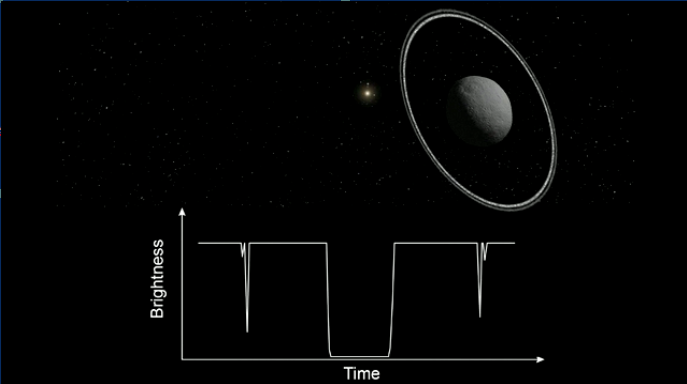
\includegraphics[scale=0.7]{pngs/curva.png}
    \caption{Representação artística de uma ocultação estelar pelo Centauro (10199)~Chariklo e seu sistema de anéis. A curva de luz esquemática (abaixo) mostra as quedas de fluxo correspondentes à passagem dos anéis e do corpo principal diante da estrela. Crédito: Lucie Maquet, 2014.}
    \label{fig:ilustracao_ocultacao}
\end{figure}

A sombra do corpo ocultante projeta-se na superfície terrestre. A precisão quilométrica decorre da combinação dessa projeção com a alta resolução temporal das observações. Cada observador, em sua posição geográfica, registra um intervalo de tempo durante o qual a estrela é ocultada - uma \textbf{corda} no plano do céu. A duração e o instante central da corda dependem da posição do observador em relação ao trajeto da sombra. Vários observadores em locais diferentes produzem várias cordas; a combinação dessas cordas permite reconstruir a forma e o tamanho do corpo no plano do céu com alta precisão \citep{SORA2022}. A previsão de ocultações depende criticamente da precisão das posições estelares e das efemérides do corpo; a melhoria contínua desses ingredientes tem ampliado o número de eventos previstos e observados, inserindo a técnica na era do \textit{big data} em astronomia \citep{SORA2022, Knieling2024}. Graças à precisão astrométrica do catálogo Gaia, o gargalo atual para a previsão de ocultações está na qualidade das efemérides dos pequenos corpos do Sistema Solar.

\begin{figure}[htbp]
    \centering
    \begin{minipage}[b]{0.48\textwidth}
        \centering
        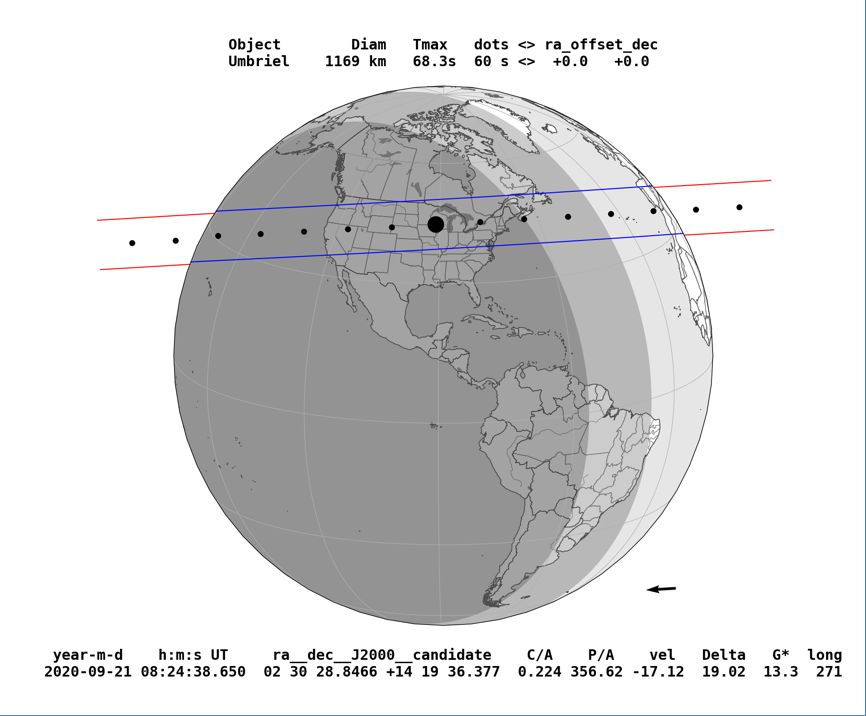
\includegraphics[width=\textwidth]{pngs/OccUmbriel_mapa.png}
        \centerline{\small (a)}
    \end{minipage}
    \hfill
    \begin{minipage}[b]{0.48\textwidth}
        \centering
        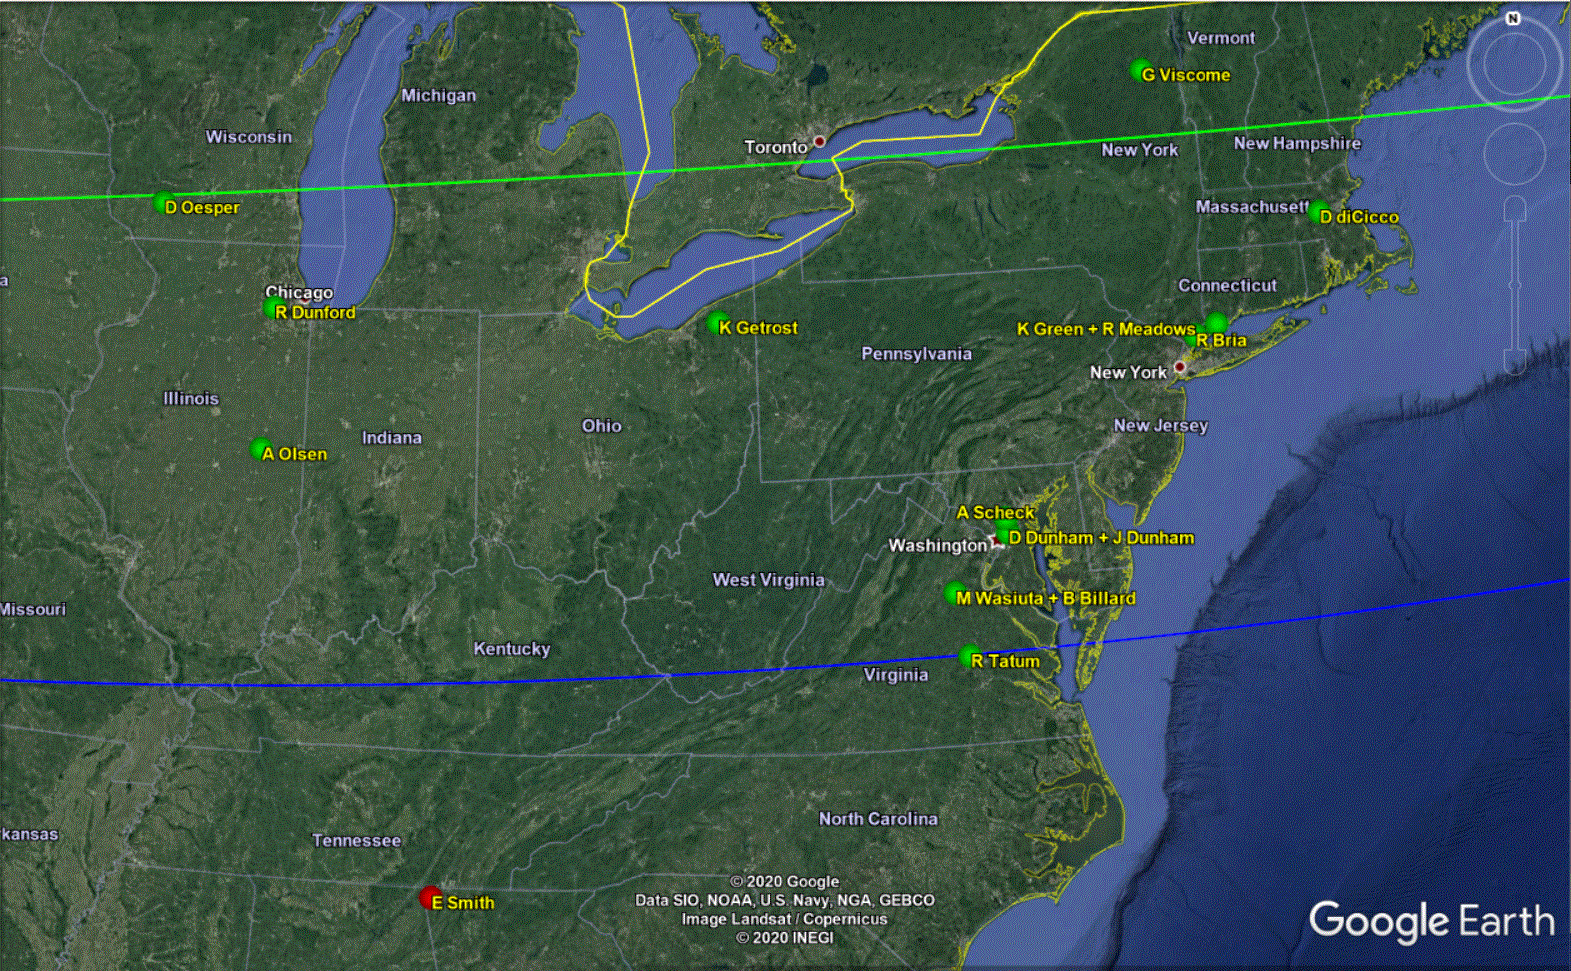
\includegraphics[width=\textwidth]{pngs/OccUmbriel_mapa2.png}
        \centerline{\small (b)}
    \end{minipage}

    \vspace{0.4cm}

    \begin{minipage}[b]{0.48\textwidth}
        \centering
        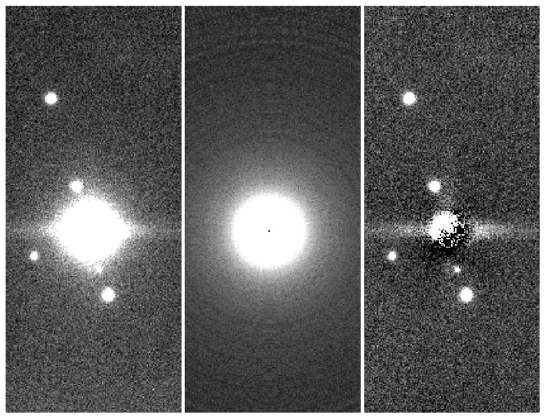
\includegraphics[width=\textwidth]{pngs/OccUmbriel_outputExemplo.png}
        \centerline{\small (c)}
    \end{minipage}
    \hfill
    \begin{minipage}[b]{0.48\textwidth}
        \centering
        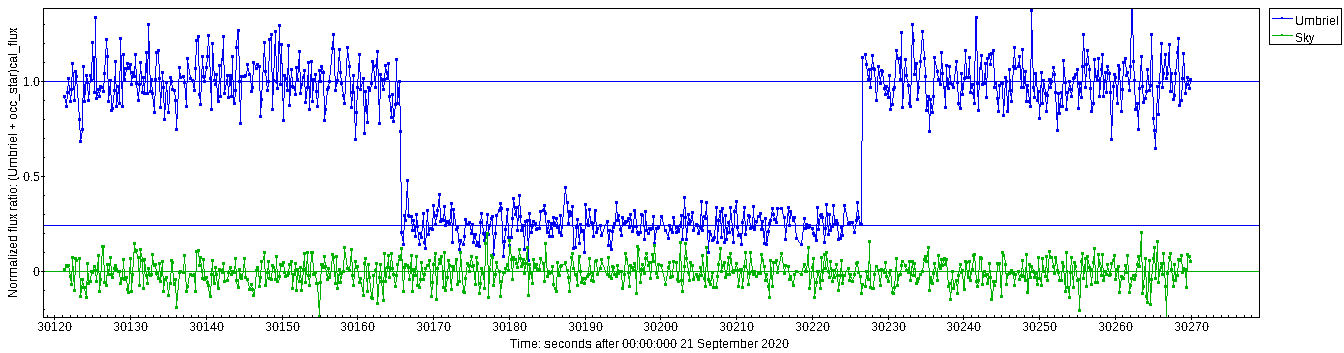
\includegraphics[width=\textwidth]{pngs/OccUmbriel_outputExemplo2.png}
        \centerline{\small (d)}
    \end{minipage}
    \caption{Exemplo completo do fluxo observacional: ocultação estelar por Umbriel (satélite de Urano), observada em 21 de setembro de 2020 \citep{Umbriel2020}. (a)~Mapa de previsão da sombra sobre a superfície terrestre. (b)~Detalhe do posicionamento dos observadores na costa leste dos EUA (Google Earth). (c)~Exemplo de quadros CCD obtidos por uma das estações: são imagens como estas que alimentam os pacotes de fotometria (e.g.\ PRAIA) para a construção das curvas de luz. Neste caso, o brilho intenso de Urano exigiu a aplicação de coronagrafia digital para viabilizar a fotometria precisa de Umbriel. (d)~Curva de luz resultante da redução via PRAIA: fluxo normalizado de Umbriel (azul) e ruído de fundo (verde), com a queda de ocultação claramente visível.}
    \label{fig:umbriel_painel}
\end{figure}

A observação é tipicamente feita por telescópios amadores e profissionais, com detectores CCD ou câmeras de vídeo. A análise das imagens serve-se de \textbf{fotometria diferencial}: mede-se o fluxo da estrela alvo em relação a estrelas de referência no mesmo campo, de modo a cancelar efeitos sistemáticos, tendo em conta a curta duração do evento (extinção atmosférica, variações de transparência). O resultado da fotometria, ao longo do tempo, é uma \textbf{curva de luz} - a série temporal do fluxo (ou razão de fluxos) em função do tempo. Em uma detecção \textbf{positiva}, a curva exibe um trecho de fluxo aproximadamente constante (estrela ainda não ocultada), uma queda relativamente abrupta (ingresso da estrela atrás do corpo), um patamar baixo (ocultação total ou parcial) e o retorno ao fluxo total da estrela (egresso). Em uma detecção \textbf{negativa}, não há queda significativa; a curva permanece estável (ou com flutuações de ruído), e essa informação é igualmente útil para dar um limite superior ao tamanho da sombra e refinar modelos. A análise detalhada da curva (ajuste de modelos que incluem diâmetro aparente da estrela, difração de Fresnel e tempo de exposição) permite obter os instantes de imersão e emersão com alta precisão e, a partir deles, as dimensões e a forma do corpo \citep{SORA2022}.



% ---------------------------
\section{Da observação às curvas de luz: coleta e armazenamento}
\label{sec:coleta_armazenamento}

As curvas de luz utilizadas em campanhas de ocultações provêm de redes de telescópios (profissionais e amadores) que registram o fluxo da estrela alvo em cadência rápida (exposições de fração de segundo a poucos segundos, com o mínimo possível de tempo morto) para maximizar a resolução temporal e, portanto, espacial ao longo da corda. O volume de dados gerado é grande: cada observação pode produzir milhares de quadros e da ordem de gigabytes por evento \citep{Cazeneuve2023}. A redução fotométrica (extração do fluxo em cada quadro) é feita com pacotes dedicados, como o PRAIA (\textit{Package for the Reduction of Astronomical Images Automatically}), que automatiza a fotometria de abertura e a construção da curva de luz a partir das imagens \citep{Assafin2023}. O SORA (\textit{Stellar Occultation Reduction and Analysis}) é utilizado na etapa de análise e redução pós-fotometria para ajuste de modelos às curvas e extração de parâmetros físicos; sua saída pode alimentar bancos de dados e catálogos (como os do Grupo do Rio). Após a redução, as curvas são armazenadas em bancos de dados ou catálogos (por exemplo, VizieR, bancos de grupos de pesquisa), em formato tabular: cada registro associa uma observação a uma série de pontos (tempo, fluxo), além de metadados (objeto ocultante, data, observador, classificação positiva/negativa quando disponível).

Nesta dissertação, a \textit{pipeline} de detecção (Capítulo 4) parte de curvas \textbf{já reduzidas} (pós-PRAIA/pós-SORA ou equivalentes), obtidas de fontes externas (Grupo do Rio, VizieR) e inseridas em um banco de dados relacional. Ou seja, o fluxo aqui descrito começa após a etapa de redução fotométrica e análise; a estrutura do banco, o fluxo de aquisição e a normalização do fluxo são detalhados no Capítulo 4. Aqui basta destacar que as curvas de luz são o insumo central para a etapa de classificação por ML: cada curva será convertida em um vetor de características e classificada como positiva ou negativa pelos modelos descritos no Capítulo 3.

% ---------------------------
\section{Características das curvas de luz e detecção positiva/negativa}
\label{sec:caracteristicas_curvas}

Do ponto de vista observacional, uma curva de luz de ocultação é uma série temporal de fluxo (normalmente normalizado em relação ao nível fora da ocultação). Sua \textbf{morfologia} depende de vários fatores físicos e instrumentais.

\textbf{Detecção positiva e negativa.} Em uma detecção positiva, a curva exibe uma queda de fluxo durante o intervalo de tempo em que o trânsito ocorre. A profundidade da queda está relacionada à fração do disco estelar ocultada e à geometria da corda; em ocultações centrais ou próximas do centro, a queda pode ser total (fluxo próximo de zero no patamar). Em uma detecção negativa, o observador está fora da sombra; a curva não apresenta queda significativa, apenas flutuações típicas de ruído fotométrico, atmosférico e instrumental. Tanto positivas quanto negativas são úteis: as primeiras fornecem cordas para o ajuste de forma e tamanho; as segundas ajudam a delimitar a borda da sombra e a descartar falsos positivos \citep{SORA2022}.

\textbf{Fatores que afetam a forma da curva.} O perfil da queda (ingresso e egresso) é influenciado pelo \textbf{diâmetro aparente da estrela} à distância do corpo ocultante: estrelas cujo diâmetro angular não é desprezível nessa escala produzem, em combinação com o ciclo de integração do detector, uma transição suave entre o nível desocultado e o ocultado. A \textbf{difração de Fresnel} nas bordas do corpo suaviza adicionalmente as regiões de ingresso e egresso; a escala típica é da ordem de \(f = \sqrt{D\lambda/2}\), onde \(D\) é a distância entre o observador e o corpo ocultante (ou, em convenções equivalentes, a distância estrela--corpo) e \(\lambda\) o comprimento de onda \citep{Roques1987}. Essa suavização faz com que os instantes de ``meia-luz'' não coincidam exatamente com o contato geométrico do limbo; exposições longas ou baixa resolução temporal podem mascarar os detalhes da difração e reduzir a precisão da extração dos tempos de imersão e emersão \citep{SORA2022}. O \textbf{tempo de exposição} converte-se em resolução espacial ao longo da corda por meio da relação \(r_t = V_S \times t_{\mathrm{exp}}\), onde \(r_t\) é a resolução espacial efetiva, \(V_S\) é a velocidade da sombra projetada na superfície terrestre e \(t_{\mathrm{exp}}\) é o tempo de exposição; exposições longas podem suavizar ou mascarar detalhes da difração. Em corpos com atmosfera, refração e absorção modificam o perfil da curva e permitem inferir composição e estrutura da atmosfera (perfis de temperatura e densidade em função da altitude) \citep{Sicardy2016}; anéis ou satélites podem produzir quedas adicionais ou assimetrias \citep{BragaRibas2014}. Para a detecção automatizada por ML, o que importa é que curvas com ocultação exibem uma queda sustentada e característica no fluxo, ao passo que curvas negativas ou com apenas ruído não exibem esse padrão; flutuações atmosféricas ou instrumentais podem, no entanto, imitar quedas pontuais, o que torna a tarefa de classificação não trivial e motiva o uso de modelos treinados e de características bem escolhidas (Capítulos 3 e 4).

\textbf{Relação sinal-ruído e qualidade.} A confiabilidade da detecção e da extração de parâmetros físicos depende da relação sinal-ruído (S/N) da curva. Em astronomia, muitas medições são feitas no limite da detectabilidade instrumental, onde o ruído pode produzir excursões que imitam fontes tênues; definições operacionais claras de detecção e critérios estatísticos são essenciais para interpretar os dados de forma confiável \citep{Wall2003}. S/N alto favorece a identificação clara da queda e a precisão dos instantes de imersão e emersão; curvas com S/N baixo são mais difíceis de classificar e mais suscetíveis a falsos positivos e negativos. Na \textit{pipeline} desta dissertação, as características extraídas de cada curva (estatísticas de fluxo, derivadas, métricas de forma, etc.) são escolhidas de forma a capturar padrões discriminativos entre curvas com e sem ocultação, mesmo na presença de ruído; o conjunto preciso de \textit{features} e o protocolo de treinamento são apresentados no Capítulo 4.

\begin{figure}[htbp]
    \centering
    \begin{minipage}[b]{0.48\textwidth}
        \centering
        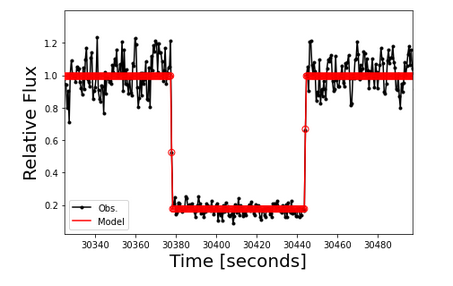
\includegraphics[width=\textwidth]{pngs/Bardecker12.png}
        \centerline{\small (a)}
    \end{minipage}
    \hfill
    \begin{minipage}[b]{0.38\textwidth}
        \centering
        
\includegraphics[scale=0.28]{Tese/pngs/LimbFitCircle.png}
        \centerline{\small (b)}
    \end{minipage}
    \caption{(a)~Curva de luz observada (preto) e modelo ajustado (vermelho) para uma das cordas da ocultação por Umbriel em 2020; os instantes de imersão e emersão, marcados por circunferências, definem a geometria da corda \citep{Umbriel2020}. (b)~Perfil do limbo de Umbriel; cada linha azul (incerteza vermelho) corresponde a uma corda projetada no plano do céu \citep{Umbriel2020}.}
    \label{fig:curvas_cordas}
\end{figure}




\textbf{Exemplo numérico: escala de Fresnel.} Para um objeto transnetuniano (TNO) a uma distância típica de $D = 40$\,UA $\approx 6{,}0 \times 10^{12}$\,m, observado no visível ($\lambda = 500$\,nm), a escala de Fresnel é
\[
f = \sqrt{\frac{D\lambda}{2}} \approx \sqrt{\frac{6{,}0 \times 10^{12} \times 5{,}0 \times 10^{-7}}{2}} \approx 1{,}2\;\text{km}.
\]
Essa escala define a resolução espacial efetiva na direção perpendicular à corda: detalhes menores que $f$ são suavizados pela difração. Ainda assim, trata-se de uma resolução da ordem de quilômetros a dezenas de unidades astronômicas de distância - superior à de qualquer telescópio óptico terrestre operando por imageamento direto. É essa capacidade de resolução que torna as ocultações estelares uma ferramenta única para a caracterização de pequenos corpos do Sistema Solar.

\begin{figure}[htbp]
    \centering
    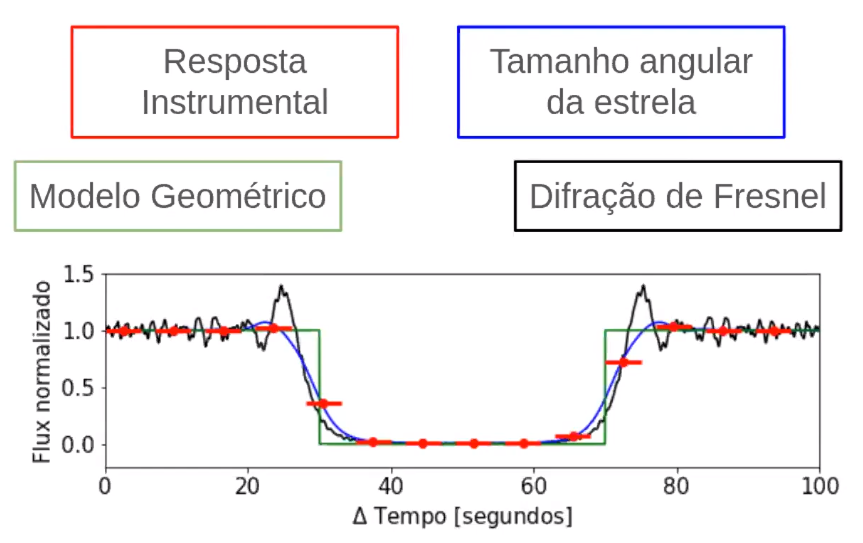
\includegraphics[width=0.55\linewidth]{pngs/ModelosSORA.png}
    \caption{Componentes do modelo de curva de luz utilizado pelo SORA \citep{SORA2022}: difração de Fresnel (azul), tamanho angular da estrela, ciclo de integração do detector e, resultante da combinação dessas componentes, o modelo geométrico (verde). O ajuste simultâneo aos dados observados (pontos vermelhos) permite determinar com precisão os instantes de imersão e emersão, necessários para a reconstrução da forma do corpo.}
    \label{fig:modelo_sora}
\end{figure}

% ---------------------------
\section{Considerações finais do capítulo}
\label{sec:consideracoes_cap2}

Este capítulo situou as ocultações estelares como fenômeno astronômico e as curvas de luz como produto observacional central. Foi destacado o papel da geometria da sombra, das cordas e da precisão astrométrica (Gaia, efemérides) na previsão e no aproveitamento dos eventos; a coleta e o armazenamento dos dados foram descritos em linhas gerais, com remissão ao Capítulo~4 para a arquitetura da \textit{pipeline} e do banco de dados; e foram resumidas as características observacionais das curvas (positiva vs.\ negativa, fatores que afetam a forma, S/N). O volume crescente de dados produzidos por redes de telescópios e catálogos como o Gaia torna \st{inviável} \textcolor{red}{penosa} a triagem manual de todas as curvas de luz; essa escala motiva o desenvolvimento de métodos automatizados de detecção baseados em aprendizado de máquina, cujos fundamentos são apresentados no Capítulo~3 e cuja implementação é detalhada no Capítulo~4. \textcolor{red}{(veja se a frase a seguir se aplica). Notadamente, nos interessam também que sejam apontados eventos tênues e que passaram desapercebidos num primeiro tratamento de curvas de luz (cite aqui os aneis de Quaoar). Um alerta confiável nesses casos é suporte para campanhas observacionais e descobertas importantes.}


\chapter{Modelos e algoritmos para Machine Learning}

% =============================================================================
% Capítulo 3 — Modelos de Machine Learning para Classificação e Agrupamento
% =============================================================================

 O Capítulo~2 mostrou que as campanhas de ocultação estelar podem produzir diversas curvas de luz, sendo número suficiente para que haja dificuldade na análise completa e minuciosa. Cada curva pode ser resumida por um conjunto de características como profundidade da queda, estatísticas de ruído, entre outros. A questão é: \emph{a partir dessa descrição numérica de uma curva, é possível decidir automaticamente se ela contém ou não uma ocultação?} Trata-se de um problema de \textbf{classificação binária}, e os métodos de \textit{Machine Learning} são as ferramentas naturais para resolvê-lo. \ia{Com isso, os objetivos deste capítulo são: definir e situar os modelos de Machine Learning como ferramentas de descobertas e classificações no contexto científico; formalizar o problema de classificação (espaço de atributos, rótulos, regiões de decisão); apresentar os principais modelos utilizados na \textit{pipeline}; e, por fim, discutir algoritmos de otimização, engenharia de características, validação de modelos e os riscos de falsos resultados.}

% -----------------------------------------------------------------------------
\section{Conceitos fundamentais de Machine Learning}
\label{sec:fundamentos_ml}

\subsection{Definição e papel do aprendizado de máquina}

O \textit{Machine Learning} (ML), ou aprendizado de máquina, é uma área na qual os sistemas "aprendem" a partir de dados, sem serem explicitamente programados para cada tarefa \citep{geron2019maos}. Em vez de regras fixas codificadas à mão, um algoritmo de ML é alimentado com informações e \textbf{ajusta seus próprios parâmetros} (por exemplo, coeficientes de uma combinação linear) para capturar padrões ou relações nos dados. Esse processo de ajuste é o que se chama de \textbf{treinamento}; ao final, o modelo está "treinado" e pode ser aplicado a novas informações. O objetivo é permitir que o sistema melhore seu desempenho à medida que mais dados ou mais iterações estejam disponíveis, especialmente em problemas sem solução analítica fechada ou com grandes volumes de dados.

No contexto científico, o ML costuma ser visto como "caixa-preta" que produz previsões sem explicação. Essa visão reflete usos industriais em que a precisão preditiva prevalece sobre a interpretabilidade. Em ciência, porém, o ML pode ir além: atuando como ferramenta de descoberta, revelando padrões que podem ser incorporados a uma teoria formal de causa e efeito. O papel do ML não é substituir a teoria, mas auxiliar na sua formulação, identificando os padrões que a teoria buscará explicar. Segundo \cite{lopez2020ml}, por exemplo, o uso do ML na ciência pode ser agrupado em algumas funções típicas:

\textbf{Sugerir a existência de algo novo:} ML pode encontrar padrões não previstos, indicando a existência de relações ainda não descobertas. Em matemática, algoritmos já auxiliaram a conjecturar teoremas que depois foram demonstrados formalmente \citep{gryak2018conjugacy}.

\textbf{Descobrir o grau de importância das variáveis:} técnicas como \textit{Mean Decrease Accuracy} (MDA) permitem avaliar o impacto de cada variável (\textbf{feature}, ou característica numérica de entrada) na predição. A ideia é treinar o modelo, medir o desempenho (por exemplo, via acurácia), embaralhar uma variável por vez e verificar se o desempenho cai; se cair, a variável é importante \citep{liu2004comparative}. Assim, o ML identifica quais variáveis devem compor explicações teóricas, mesmo sem revelar o mecanismo causal.

\textbf{Explorar relações de causa e efeito:} um modelo pode ser ajustado com dados nos quais um determinado efeito está ausente. Depois, quando esse efeito passa a atuar, o modelo continua produzindo previsões baseadas no cenário anterior. Se as observações reais passarem a divergir das previsões, essa diferença pode ser um indício de que o efeito alterou o sistema, sugerindo possíveis relações causais.

\textbf{Redução e simplificação:} em dados multidimensionais, técnicas de redução de dimensionalidade — por exemplo, a Análise de Componentes Principais (PCA) — projetam os dados em um espaço de menor dimensão, tornando mais evidentes padrões, agrupamentos e relações entre observações, o que favorece a interpretação dos resultados.

\textbf{Encontrar padrões desconhecidos:} o ML pode atuar na detecção de eventos raros ou anomalias em grandes volumes de dados - por exemplo, na triagem automática de ocultações estelares em levantamentos astronômicos - indicando onde vale a pena investigar, mesmo sem explicar o mecanismo.

Neste trabalho, o ML atua sobretudo na função de \textbf{encontrar padrões desconhecidos} e de \textbf{descobrir o grau de importância das variáveis} (importância das \textit{features} nos ensembles de árvores), em apoio à decisão do pesquisador sobre quais curvas merecem análise detalhada.

\subsection{Aprendizado supervisionado versus não supervisionado}

A taxonomia usual divide o ML em dois cenários, conforme a natureza dos dados:

\begin{itemize}
	\item \textbf{Supervisionado:} cada exemplo possui um rótulo (classe ou valor numérico). Tarefas típicas: classificação (rótulo discreto) e regressão (rótulo contínuo). Exemplos: filtro de spam, previsão de preços.
	\item \textbf{Não supervisionado:} os dados não possuem rótulos. Tarefas típicas: agrupamento (clustering), detecção de anomalias, redução de dimensionalidade. Exemplos: segmentação de clientes, identificação de \textit{outliers} (anomalias).
\end{itemize}

Neste trabalho, o foco é o \textbf{paradigma supervisionado}, em particular a \textbf{classificação binária}. No aprendizado supervisionado, o objetivo é encontrar uma função \(f\) que mapeie cada entrada \(\vec{x}\) (por exemplo, o vetor de características de uma curva de luz) a um rótulo \(y\) (por exemplo, "ocultação presente" ou "ausente"). Os rótulos usados no treinamento vêm da classificação já conhecida dos dados (a chamada \textbf{verdade de campo}, ou \textit{ground truth} - por exemplo, a análise prévia de um especialista ou o catálogo). O objetivo é que \(f\) \textbf{generalize} bem, ou seja, que erre pouco em dados novos que não foram usados no ajuste. A detecção de ocultações estelares é formulada exatamente assim: a curva de luz contém um evento de ocultação (classe positiva, \(y=1\)) ou não (classe negativa, \(y=0\)). Os classificadores (Regressão Logística, Random Forest, XGBoost, CatBoost) recebem vetores de características extraídos das curvas e produzem uma classe ou uma probabilidade de classe, permitindo triagem e priorização automáticas no fluxo da \textit{pipeline} \ia{(Capítulo 4)}.

% -----------------------------------------------------------------------------
\section{O problema da classificação supervisionada}
\label{sec:problema_classificacao}
\label{sec:reglin_didatica}

Em notação matemática, uma amostra rotulada é representada pela tupla \(Z = (X, Y)\). Aqui \(X = \{\vec{x}_1, \vec{x}_2, \ldots, \vec{x}_n\}\) é o conjunto de \textbf{vetores de características}: cada \(\vec{x}_i \in \mathbb{R}^d\) é um vetor com \(d\) números que resumem, no caso deste trabalho, uma curva de luz (amplitude, mínimo do fluxo suavizado, distância entre centróides, etc.). O número \(d\) é a "dimensionalidade'' do problema (neste caso, 14 ou 28 features). O conjunto \(Y = \{y_1, y_2, \ldots, y_n\}\) contém os \textbf{rótulos}: a classificação verdadeira de cada exemplo, com \(y_i \in \{0,1\}\) no caso binário (0 = sem ocultação, 1 = com ocultação).

Um \textbf{classificador} é uma função \(f \colon \mathbb{R}^d \longrightarrow \{0,1\}\) (ou, em geral, \(\{1,\ldots,c\}\) para \(c\) classes) que, dado um vetor \(\vec{x}\), prediz um rótulo \(y\). Em muitos modelos, \(f\) produz primeiro uma \textbf{probabilidade} de a classe ser positiva; a decisão final é então "positivo"~se essa probabilidade for maior ou igual a 50 \%, e "negativo"~caso contrário. O uso do valor 0,5 é intuitivo, mas cabe frisar que é arbitrário e dependerá do objetivo do modelo que está sendo treinado (esse limite decisório é chamado de 'threshold' nas pipelines de ML, ou $\tau$, e será melhor explorado mais adiante). 

A função \(f\) divide o espaço \(\mathbb{R}^d\) em \textbf{regiões de decisão}: \(R_k = \{\vec{x} \in \mathbb{R}^d \mid f(\vec{x}) = k\}\). Cada região corresponde a uma classe. O objetivo do treinamento é estimar \(f\) a partir dos dados \((X,Y)\) de modo que \(f\) generalize bem para novos exemplos não vistos.

Antes de apresentar os modelos de classificação, convém fixar a ideia de treinamento como minimização de uma função de custo. O exemplo mais natural de ser explorado é a \textbf{regressão linear}. O modelo $y_i = \beta_0 + \beta_1 x_i + \epsilon_i$ descreve o comportamento médio de uma variável resposta $y$ dado $x$, com erro $\epsilon_i$ (Figura~\ref{fig:linear}).

\begin{figure}[htbp]
\begin{center}
	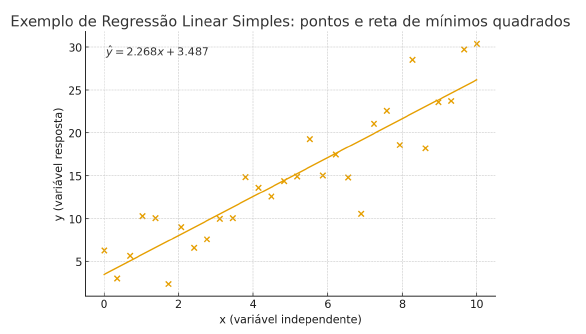
\includegraphics[scale=0.9]{pngs/exemplo_regressaoLinear.png}
\caption{Exemplo ilustrativo de regressão linear simples (dados genéricos, não referentes a curvas de luz de ocultação) \citep{Levada2026}.}
\label{fig:linear}
\end{center}
\end{figure}

Os parâmetros são estimados pelo método dos \textbf{mínimos quadrados}, que constitui o primeiro exemplo de algoritmo de otimização nesta dissertação. No caso mais simples ($\mathbb{R}^2$), o modelo é $y = \alpha + \beta x$ e a função de custo é
\[
J(\alpha,\beta) = \sum_{i=1}^{n} (y_i - \alpha - \beta x_i)^2,
\]
minimizada pela condição $\partial J / \partial \alpha = 0$, $\partial J / \partial \beta = 0$. A generalização para múltiplas variáveis ($d$ dimensões) segue naturalmente em notação vetorial. O modelo prediz $\hat{\vec{y}} = X\vec{\theta}$, com $X$ a matriz de dados (cada linha é um exemplo, cada coluna uma variável) e $\vec{\theta}$ o vetor de parâmetros. A função de custo torna-se
\[
J(\vec{\theta}) = (\vec{y} - X\vec{\theta})^\top (\vec{y} - X\vec{\theta}) = \sum_{i=1}^{n} \big( y_i - \vec{\theta}^\top \vec{x}_i \big)^2.
\]
A condição de mínimo, $\nabla_{\vec{\theta}} J = \vec{0}$, fornece a \textbf{equação normal}:
\[
X^\top (X\vec{\theta} - \vec{y}) = \vec{0} \quad \Longrightarrow \quad \vec{\theta}^* = (X^\top X)^{-1} X^\top \vec{y}.
\]
Após estimar $\vec{\theta}^*$, o modelo pode predizer $\vec{y}$ para novos dados de entrada \citep{geron2019maos, Levada2026}.

Apesar dos problemas de regressão servirem de excelente passo inicial para se compreender as métricas e interpretações básicas dos modelos de ML, para problemas de classificação, não usamos regressão linear diretamente - a solução completa desses problemas podem ser acompanhadas no capítulo 2 de \citep{Levada2026}. A \textbf{Regressão Logística} mantém a combinação linear, mas mapeia a saída ao intervalo $(0,1)$ por uma função sigmoide e utiliza o custo de entropia cruzada, para o qual \ia{\textbf{não existe solução fechada}} (o treinamento é feito por algoritmos iterativos - Seção~\ref{sec:otimizacao}).

% -----------------------------------------------------------------------------
\section{Modelos de classificação utilizados na pipeline}
\label{sec:modelos_classificacao}

\subsection{Regressão Logística}

A Regressão Logística é um classificador probabilístico. Similarmente à Regressão Linear, este modelo calcula uma soma ponderada das características de entrada, mas, em vez de gerar o resultado diretamente, gera a \textit{logística} (função sigmoide) desse resultado \citep{geron2019maos}. Em outras palavras, ele transforma combinações lineares de características em probabilidades válidas.

Suponha um problema de classificação no qual se deseja identificar uma ocultação em uma curva de luz a partir de uma única informação: o \textbf{tamanho da queda máxima do fluxo}. Curvas com maiores quedas possuem maior probabilidade de conter a ocultação. A figura a seguir ilustra a aplicação da regressão linear em dados bem comportados.

\begin{figure}[htbp]
    \centering
    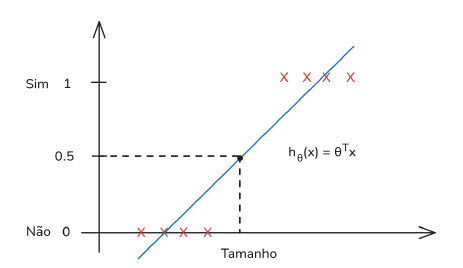
\includegraphics[width=0.5\linewidth]{pngs/regressao_linear_ex1.png}
\caption{Aplicação da regressão linear ao problema de classificação binária: a reta produz saídas fora do intervalo $[0,1]$ \citep{Levada2026}. Nosso conjunto de dados mostra quatro amostras de curvas de luz com grandes amplitudes e outras quatro com baixas amplitudes. Nesse exemplo simples, o valor de 0,5 para o recorte da reta divide perfeitamente as duas classificações.}
    \label{fig:reglin_classif_ex1}
\end{figure}

Nesse caso, teríamos infinitos valores sob uma reta para a variável de saída. \ia{Notadamente,} a solução mais intuitiva seria considerar um limiar simples na metade da reta. No entanto, suponha que, no mesmo conjunto de dados, tivéssemos um elemento \textit{outlier}, uma anomalia. A Figura~\ref{fig:reglin_classif_ex2} ilustra a situação: o limiar que antes funcionava deixa de ser útil, pois agora a metade da reta passa a considerar um ponto positivo como negativo ao mesmo tempo que varios pontos positivos ficam proximos do limiar de decisão (e apenas o outlier se encontra confortavelmente longe das curvas consideradas negativas), gerando dúvida para o analista que estuda os dados.

\begin{figure}[htbp]
    \centering
    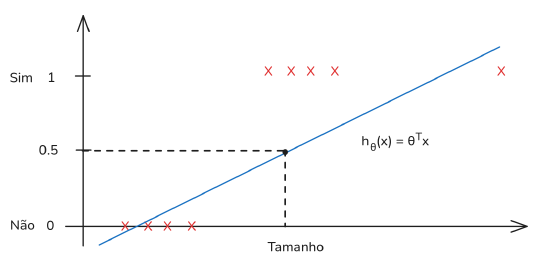
\includegraphics[width=0.5\linewidth]{pngs/regressao_linear_ex2.png}
    \caption{O mesmo problema anterior, mas com a adição de um \textit{outlier}. Uma das curvas possui tamanho de amplitude muito diferente da escala normal, possivelmente resultado da falta de normalização. Veja como a reta de regressão se desloca e o limiar 0,5 passa a classificar incorretamente \citep{Levada2026}.}
    \label{fig:reglin_classif_ex2}
\end{figure}

O que podemos ver é a reta de regressão pode sofrer alterações significativas com a inclusão de novos pontos, evidenciando sua sensibilidade aos dados observados. \ia{Além disso,} a regressão linear pode gerar valores fora do intervalo [0,1], incompatíveis com a interpretação probabilística. \ia{Dessa forma,} sua sensibilidade a outliers e a ausência de uma saída naturalmente probabilística fazem da regressão linear uma abordagem inadequada para tarefas de classificação.

\ia{Nesse sentido,} a regressão logística funcionará de forma similar a modelos lineares (saída contínua), mas será adaptado. O primeiro ponto será a interpretação probabilística: a combinação linear \(\vec{\theta}^\top \vec{x}\) será mapeada pela logística ao intervalo \((0,1)\), permitindo a interpretação como a probabilidade da classe ser positiva \citep{Levada2026}. 

Em notação vetorial, seja \(\vec{\theta}\) o vetor de parâmetros  e \(\vec{x}\) o vetor de atributos; a probabilidade predita é
\[
\hat{p} = h_{\vec{\theta}}(\vec{x}) = \sigma(\vec{\theta}^\top \vec{x}) = \frac{1}{1 + e^{-\vec{\theta}^\top \vec{x}}}.
\]
A decisão é: classe 1 se \(\hat{p} \geq 0{,}5\), caso contrário classe 0. Isso pois a saída continuará continua, mas dessa vez limitada entre 0 e 1. \ia{Vale lembrar, também,} que o valor de 0,5 pode ser alterado a depender da calibração do modelo\ia{, como discutido no início do capítulo}. 

O segundo ponto a ser adaptado será quanto ao treinamento. \ia{Nesse sentido,} passa-se a utilizar outra função de custo ao invés dos mínimo quadrados: a \textbf{entropia cruzada} (ou \textit{log loss}). Essa medida penaliza predições distantes do rótulo real. Por exemplo, se temos uma curva positiva (ocultação presente), e o modelo prediz uma probabilidade baixa de haver ocultação, o custo deverá ser alto. 

\[
loss = - [y \log{p} + (1-y) \log{(1-p)}]
\] onde p é a probabilidade prevista pelo modelo e a perda (loss) deverá ser aplicada a um único ponto. Ou seja, para um conjunto de \(m\) exemplos, com rótulos \(y^{(i)} \in \{0,1\}\) e probabilidades preditas \(\hat{p}^{(i)}\), a função é
\begin{equation}
J(\vec{\theta}) = -\frac{1}{m} \sum_{i=1}^{m} \left[ y^{(i)} \log(\hat{p}^{(i)}) + (1 - y^{(i)}) \log(1 - \hat{p}^{(i)}) \right].
\end{equation}


A minimização de \(J(\vec{\theta})\) é equivalente à maximização da log-verossimilhança (MLE), de modo que os parâmetros estimados são estatisticamente ótimos sob o modelo probabilístico assumido \citep{geron2019maos, Levada2026}. O ajuste é realizado por gradiente descendente (veremos mais detalhes sobre os algoritmos de otimização na Seção~\ref{sec:otimizacao}). O gradiente de \(J\) em relação a \(\vec{\theta}\) pode ser escrito na forma vetorial
\[
\nabla_{\vec{\theta}} J(\vec{\theta}) = \frac{1}{m} X^\top \big( \sigma(X\vec{\theta}) - \vec{y} \big),
\]
onde \(X\) é a matriz de dados e \(\vec{y}\) o vetor de rótulos. A atualização dos parâmetros em cada iteração segue a \textbf{direção oposta ao gradiente} (direção de maior descida do custo), com passo controlado pela \textbf{taxa de aprendizado} \(\eta\) (análogo ao passo de um método numérico de minimização). \ia{Trata-se, portanto, de uma medida sobre o quão distante da realidade estão as previsões do modelo.}

\vspace{0.3cm}
\noindent\textbf{Exemplo numérico: uma iteração do gradiente descendente.}
Para tornar o mecanismo concreto, considere $m = 4$ curvas com uma única feature $x$ (amplitude da queda de fluxo, normalizada entre 0 e 1) e rótulos $y$ (0 = sem ocultação, 1 = com ocultação):

\begin{table}[htbp]
\centering
\small
\begin{tabular}{cccc}
\hline
Curva & $x$ & $y$ & $\hat{p}$ (inicial) \\
\hline
1 & 0{,}2 & 0 & 0{,}50 \\
2 & 0{,}4 & 0 & 0{,}50 \\
3 & 0{,}7 & 1 & 0{,}50 \\
4 & 0{,}9 & 1 & 0{,}50 \\
\hline
\end{tabular}
\caption{Dados do exemplo numérico da Regressão Logística (valores ilustrativos).}
\label{tab:exemplo_logistica}
\end{table}

Inicializamos $\theta_0 = 0$ e $\theta_1 = 0$. Como $\sigma(0) = 0{,}5$, todas as curvas recebem probabilidade $\hat{p} = 0{,}5$ e o custo inicial é $J = -\log(0{,}5) \approx 0{,}693$. Os gradientes são $\partial J / \partial \theta_0 = \frac{1}{4}\sum_i (\hat{p}_i - y_i) = 0$ e $\partial J / \partial \theta_1 = \frac{1}{4}\sum_i (\hat{p}_i - y_i)\,x_i = -0{,}15$. Com taxa de aprendizado $\eta = 1{,}0$, a atualização dá $\theta_1 \leftarrow 0 - 1{,}0 \times (-0{,}15) = 0{,}15$. Recalculando as probabilidades com o novo $\theta_1$, obtemos $\hat{p}_1 = \sigma(0{,}03) \approx 0{,}507$, $\hat{p}_2 \approx 0{,}515$, $\hat{p}_3 \approx 0{,}526$ e $\hat{p}_4 \approx 0{,}534$. O custo cai para $J \approx 0{,}685$. Uma única iteração já empurrou as probabilidades na direção correta: as curvas com maior amplitude (3 e 4, positivas) receberam $\hat{p}$ ligeiramente maior que as negativas. Após centenas de iterações, a separação se consolida.
\vspace{0.3cm}

Sem nenhuma restrição, a Regressão Logística é livre para atribuir pesos enormes a qualquer feature --- inclusive ao ruído. Se uma curva de treino por acaso tem um pico espúrio que coincide com a classe positiva, o modelo pode atribuir peso grande a essa flutuação; na hora de classificar curvas novas, esse peso exagerado prejudica a predição. Esse é o problema do \textbf{sobreajuste} (overfitting, discutido em detalhe na Seção~\ref{sec:overfitting}): o modelo ``decorou'' particularidades do treino em vez de aprender o padrão geral.

A solução é a \textbf{regularização}: impor um custo adicional aos pesos grandes, forçando o modelo a manter coeficientes moderados e a distribuir a ``explicação'' entre múltiplas \textit{features} em vez de apostar tudo em uma \citep{geron2019maos, Levada2026}. As três formas principais são:

\begin{itemize}
	\item \textbf{Ridge (\(\ell_2\)):} adiciona ao custo o termo \(\frac{\alpha}{2} \sum_j \theta_j^2\). Os coeficientes são \textit{encolhidos} em direção a zero, mas raramente se anulam - todos os atributos permanecem no modelo. Funciona bem com \textit{features} correlacionadas, reduzindo o sobreajuste sem descartar características.

	\item \textbf{Lasso (\(\ell_1\)):} adiciona \(\alpha \sum_j |\theta_j|\). Tende a \textbf{zerar} coeficientes de atributos irrelevantes, atuando como seleção automática de variáveis. Em contrapartida, pode comportar-se de forma errática com muitas variáveis correlacionadas (tendendo a escolher apenas uma) ou quando o número de variáveis supera o de instâncias. A função de custo não é diferenciável em \(\theta_j = 0\) (algoritmos de otimização não sabem a direção do próximo passo), exigindo subgradientes na otimização.

	\item \textbf{Elastic Net:} combina as penalidades Ridge e Lasso com uma taxa de mistura, unindo os benefícios de ambas. É recomendado quando há muitas variáveis correlacionadas.
\end{itemize}

Existe uma interpretação elegante dessas penalidades do ponto de vista bayesiano (Estimativa MAP --- \textit{Maximum A Posteriori}). Regularizar equivale a assumir uma crença prévia (\textit{prior}) sobre os valores dos coeficientes do modelo \emph{antes} de ver os dados. No Ridge, essa crença é uma \textbf{distribuição Gaussiana} centrada em zero: acredita-se que os pesos são provavelmente pequenos, mas não necessariamente nulos --- as caudas suaves da Gaussiana permitem valores moderados (Figura~\ref{fig:gaussLaplace}). No Lasso, a crença é uma \textbf{distribuição de Laplace}, que tem um pico afiado em zero: acredita-se que muitos pesos \emph{são} zero, e apenas alguns poucos são relevantes --- daí o efeito de seleção automática de variáveis \citep{geron2019maos, Levada2026}.

O hiperparâmetro \(\alpha\) (ou \(C = 1/\alpha\)) controla a força da penalização: \(\alpha\) grande significa uma crença prévia forte de que os pesos devem ser pequenos; \(\alpha\) pequeno deixa o modelo mais livre. A escolha de \(\alpha\) é feita por \textbf{validação cruzada}: treina-se o modelo com diferentes valores de \(\alpha\) e seleciona-se aquele de melhor desempenho médio nas partições de validação (as \emph{dobras}, ou \textit{folds}, definidas na Seção~\ref{sec:validacao_modelos}) \citep{geron2019maos}.

É essencial \textbf{escalonar} as \textit{features} (e.g.\ StandardScaler) antes de aplicar Ridge ou Lasso, pois ambas as penalidades são sensíveis à escala dos dados: um atributo medido em quilômetros terá coeficiente numericamente muito diferente do mesmo atributo medido em metros, e a penalização tratará ambos de forma desigual. Nesta dissertação, utiliza-se Ridge ou Lasso na Regressão Logística, conforme documentado no Apêndice~\ref{ap:hiperparametros}.

\begin{figure}[!h]
    \centering
    
\includegraphics[width=0.5\linewidth]{Tese/pngs/Comparison-of-Gaussian-and-Laplace-distributions.png}
    \caption{Comparação entre as distribuições Gaussiana e de Laplace, que correspondem aos priors assumidos sobre os parâmetros na interpretação bayesiana das regularizações Ridge e Lasso, respectivamente.}
    \label{fig:gaussLaplace}
\end{figure}


A Regressão Logística serve de base conceitual para entender classificadores probabilísticos e foi também treinada e avaliada na \textit{pipeline} desta dissertação, junto com os demais modelos (Random Forest, XGBoost, CatBoost), que tipicamente oferecem melhor desempenho em dados tabulares e fornecem importância de variáveis. A função sigmoide \(\sigma(z) = 1/(1+e^{-z})\) está ilustrada na Figura~\ref{fig:sigmoide}.

\begin{figure}[htbp]
\begin{center}
	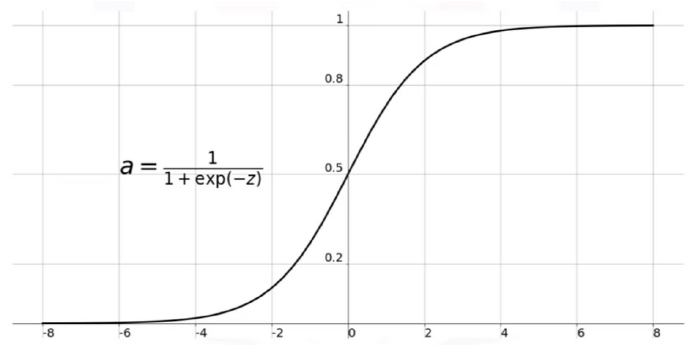
\includegraphics[scale=0.85]{pngs/sigmoide.png}
\caption{Função sigmoide \(\sigma(z) = 1/(1+e^{-z})\).}
\label{fig:sigmoide}
\end{center}
\end{figure}

\subsection{Árvores de decisão e critérios de impureza}

Os modelos Random Forest, XGBoost e CatBoost são baseados em \textbf{árvores de decisão}. Uma árvore de decisão é um classificador que funciona como um fluxograma: em cada "nó"~ pergunta-se o valor de uma das características (por exemplo, "o mínimo do fluxo suavizado é menor que 0,85?"); conforme a resposta, segue-se por um dos dois ramos até um novo nó ou até uma "folha", que devolve a classe predita. O espaço de entradas (vetores de características) fica assim particionado em regiões (hiper-retângulos), cada uma associada a uma classe \citep{Levada2026}. Uma das maiores vantagens é a \textbf{interpretabilidade}: as regras podem ser lidas e aplicadas manualmente, em contraste com modelos opacos como redes neurais. O \textit{scikit-learn} \citep{ScikitLearn2011} utiliza o algoritmo \textbf{CART} (\textit{Classification and Regression Trees}), que produz árvores binárias e escolhe, em cada nó, a divisão que maximiza a pureza dos nós filhos \citep{geron2019maos}. Os dois critérios de impureza mais usados para classificação são o \textbf{coeficiente de Gini} e a \textbf{entropia}. Para um nó \(i\) com proporções \(p_{i,k}\) de exemplos na classe \(k\) (com \(k=1,\ldots,c\) classes):
\begin{equation}
G_i = 1 - \sum_{k=1}^{c} p_{i,k}^2, \qquad
H_i = -\sum_{k=1}^{c} p_{i,k} \log_2(p_{i,k}) \quad (\text{convenção } 0\log 0 = 0).
\end{equation}
Nessas expressões, \(G_i\) é o coeficiente de Gini e \(H_i\) é a \textbf{entropia} do nó \(i\): ambos medem a impureza, ou seja, o quanto as classes estão misturadas naquele nó. Os dois valem zero quando o nó é puro (todos os exemplos pertencem a uma única classe) e crescem à medida que as classes ficam mais equilibradas entre si.

O Gini tende a isolar a classe mais frequente; a entropia tende a produzir árvores mais equilibradas. A divisão é feita de modo a maximizar a redução da impureza (ganho de informação). Árvores de decisão são instáveis e sensíveis a pequenas variações nos dados; sem restrições, tendem ao sobreajuste. Para regularizar, utilizam-se critérios de parada como profundidade máxima (\textit{max\_depth}) e número mínimo de amostras por nó ou por folha (\textit{min\_samples\_leaf}) \citep{geron2019maos}. A \textbf{poda} (\textit{pruning}) pode ser aplicada após o crescimento completo, removendo ramos que não contribuem significativamente para a capacidade preditiva \citep{Levada2026}.

\vspace{0.3cm}
\noindent\textbf{Exemplo numérico: redução de impureza de Gini em uma divisão.}
Considere um nó contendo $8$ curvas de luz de treino, sendo $4$ positivas (com ocultação) e $4$ negativas. Como as classes estão perfeitamente misturadas, a impureza é máxima para o caso binário:
\[
G_{\text{nó}} = 1 - \left[\left(\tfrac{4}{8}\right)^2 + \left(\tfrac{4}{8}\right)^2\right] = 1 - 0{,}5 = 0{,}5.
\]
A árvore testa então uma divisão candidata --- por exemplo, ``profundidade da queda $> 0{,}5$?'' --- que separa as $8$ curvas em dois nós-filhos:
\begin{itemize}
	\item \textbf{Filho da esquerda} ($3$ curvas, todas positivas): $G_{\text{esq}} = 1 - \left[1^2 + 0^2\right] = 0$ (nó \emph{puro}).
	\item \textbf{Filho da direita} ($5$ curvas, $1$ positiva e $4$ negativas): $G_{\text{dir}} = 1 - \left[\left(\tfrac{1}{5}\right)^2 + \left(\tfrac{4}{5}\right)^2\right] = 1 - 0{,}68 = 0{,}32$.
\end{itemize}
A impureza após a divisão é a média \textbf{ponderada} pelo número de exemplos em cada filho:
\[
G_{\text{div}} = \frac{3}{8}\times 0 + \frac{5}{8}\times 0{,}32 = 0{,}20,
\]
e o \textbf{ganho} (redução de impureza) é $\Delta G = G_{\text{nó}} - G_{\text{div}} = 0{,}50 - 0{,}20 = 0{,}30$. A divisão deixou os nós mais ``puros'' (o da esquerda já decide com certeza pela classe positiva). O algoritmo CART avalia todos os cortes candidatos de todas as \textit{features} e escolhe aquele que produz o \emph{maior} ganho; o processo se repete em cada nó-filho até atingir um critério de parada.
\vspace{0.3cm}

\subsection{Random Forest (Floresta Aleatória)}

Random Forest é um método de \textbf{ensemble}: em vez de uma única árvore, treina-se um grande número de árvores de decisão (por exemplo, centenas), cada uma em uma \textbf{amostra aleatória} dos dados (amostragem com reposição, ou \textit{bootstrap}) e usando, em cada divisão de nó, apenas um subconjunto aleatório das características \citep{geron2019maos, Levada2026}. A predição final é obtida por \textbf{votação majoritária}: cada árvore "vota" em uma classe e escolhe-se a classe que recebeu mais votos. A força da floresta está na \textbf{descorrelação} entre as árvores. Aqui, \textbf{\textit{bagging}} (de \textit{bootstrap aggregating}) é a técnica de treinar cada árvore em uma amostra distinta dos dados, sorteada com reposição, e depois agregar as predições por votação: como cada árvore vê um conjunto ligeiramente diferente, elas erram em casos diferentes. O \textit{bagging} e a escolha aleatória de atributos em cada nó garantem essa diversidade; ao agregar centenas de árvores, o modelo mantém o baixo viés das árvores individuais e reduz drasticamente a \textbf{variância}. Uma vantagem colateral é a estimativa \textbf{out-of-bag} (OOB): como cada árvore é treinada em aproximadamente 63\% dos dados (amostragem com reposição), cerca de 37\% das instâncias ficam "fora da bolsa"~para cada árvore e podem ser usadas como conjunto de validação interno, permitindo estimar o erro de generalização sem um conjunto de teste separado \citep{geron2019maos}. Uma variante ainda mais aleatória são as \textbf{Extra-Trees} (\textit{Extremely Randomized Trees}): em vez de procurar o melhor ponto de corte em cada atributo, sorteiam limiares ao acaso e ficam com o melhor entre os sorteados. Isso acelera o treinamento e pode reduzir ainda mais a variância, ao custo de um viés ligeiramente maior \citep{geron2019maos}.

A aleatoriedade em dois níveis --- nos dados e nos atributos --- reduz a correlação entre as árvores e diminui a \textbf{variância} do ensemble: ao agregar predições de árvores pouco correlacionadas, o erro global tende a ser menor que o de uma única árvore \citep{geron2019maos}. O \textbf{Teorema do Júri de Condorcet} ilustra a ideia: se cada "votante" (árvore) tem probabilidade maior que 50\% de acertar, a decisão por maioria tende a melhorar com o número de votantes. Por exemplo, várias árvores com acurácia individual em torno de 65\% podem produzir um ensemble com acurácia bem maior (da ordem de 90\% ou mais), desde que os erros não sejam idênticos. O ganho depende da \textbf{diversidade} entre os modelos: se todos errarem nos mesmos casos, a votação não corrige.

Além da predição, Random Forest fornece uma estimativa natural da \textbf{importância das variáveis} (por exemplo, pela queda média na impureza ou na acurácia quando a variável é permutada), o que é útil para análise exploratória e seleção de features (Capítulo 4). Nesta dissertação, a importância das variáveis nos modelos baseados em árvores (Random Forest, XGBoost, CatBoost) é obtida pela \textbf{queda média na impureza} (Gini) em cada divisão em que a variável participa; para a Regressão Logística, utilizam-se os coeficientes estimados (em valor absoluto ou normalizado). \ia{O critério adotado na \textit{pipeline} é detalhado no Capítulo 4, e os resultados (ranking e magnitude das importâncias) são apresentados no Capítulo 5.}

\begin{figure}[htbp]
\begin{center}
	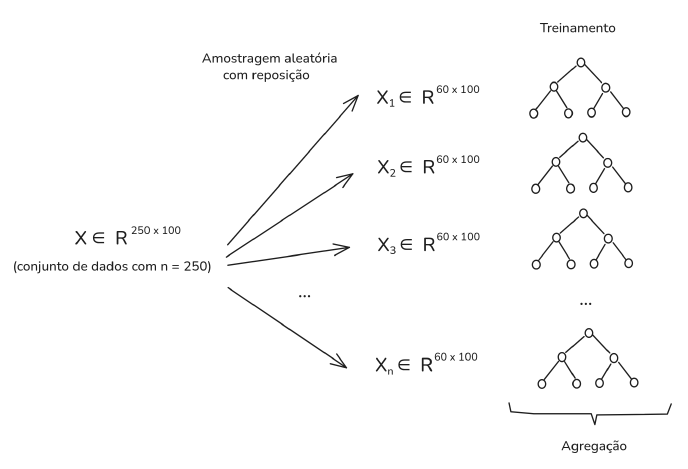
\includegraphics[scale=0.95]{pngs/RF_img.png}
\caption{Esquema simplificado do funcionamento de uma Floresta Aleatória.}
\label{fig:random_forest}
\end{center}
\end{figure}

\begin{figure}[htbp]
\begin{center}
	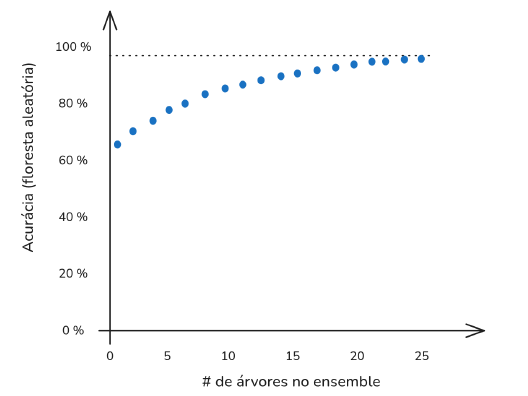
\includegraphics[scale=0.85]{pngs/manual_2.png}
\caption{Exemplo ilustrativo: 25 árvores com acurácia individual em torno de 65\% podem resultar em uma floresta com acurácia de aproximadamente 94\%.}
\label{fig:ensemble_acuracia}
\end{center}
\end{figure}

\subsection{XGBoost (eXtreme Gradient Boosting)}

O \textbf{boosting} é uma família de métodos em que os modelos são treinados \textbf{um após o outro}: cada novo modelo (por exemplo, uma árvore) é ajustado para corrigir os erros do modelo anterior, de modo que a combinação de todos forme um preditor forte a partir de vários preditores "fracos" \citep{geron2019maos, Levada2026}. O \textbf{gradient boosting} utiliza um modelo aditivo: na iteração \(m\),
\begin{equation}
F_m(\vec{x}) = F_{m-1}(\vec{x}) + \eta \, h_m(\vec{x}),
\end{equation}
onde \(h_m\) é um novo aprendiz fraco (por exemplo, uma árvore rasa) ajustado ao \textbf{gradiente negativo} da função de perda em relação à predição atual \(F_{m-1}\) --- ou seja, aos "resíduos" no espaço da perda \citep{geron2019maos}. A taxa de aprendizado \(\eta\) controla a contribuição de cada árvore (encolhimento, \textit{shrinkage}), reduzindo o risco de overfitting. O XGBoost (\textit{eXtreme Gradient Boosting}) aprimora esse esquema ao adicionar termos de regularização explícitos na função de custo (penalizando o número de folhas e os pesos das folhas) e ao utilizar uma expansão de Taylor de segunda ordem da perda para otimizar a atualização de cada árvore, o que resulta em implementação eficiente e alto desempenho \citep{geron2019maos}.

O XGBoost tornou-se muito popular em competições e aplicações práticas por sua precisão e velocidade. Em contraste com o Random Forest (que treina árvores em paralelo), o boosting é inerentemente sequencial, o que pode limitar o paralelismo em certas fases, mas o ganho de desempenho preditivo costuma compensar. \ia{Na \textit{pipeline} desta dissertação, o XGBoost é um dos quatro classificadores treinados e avaliados (Regressão Logística, Random Forest, XGBoost, CatBoost) (Capítulo 4).}

\subsection{CatBoost}

CatBoost (\textit{Categorical Boosting}) é um algoritmo de \textit{gradient boosting} baseado em árvores, desenvolvido pela Yandex, que incorpora inovações voltadas à robustez e à eficiência do treinamento.

Assim como o XGBoost, o CatBoost constrói árvores sequencialmente, minimizando uma função de perda por gradiente. Entretanto, difere em dois aspectos arquiteturais relevantes:

\begin{itemize}
	\item \textbf{\textit{Ordered Boosting}:} para calcular os resíduos de cada exemplo, o CatBoost utiliza apenas os modelos treinados com exemplos anteriores a ele (em uma permutação aleatória do conjunto), combatendo o \textit{target leakage} (vazamento de rótulo) --- situação em que a predição de um exemplo é influenciada pelo próprio rótulo durante o treinamento. Esse procedimento reduz o viés otimista na estimativa dos resíduos, especialmente em conjuntos pequenos ou moderados.

	\item \textbf{\textit{Oblivious Decision Trees}:} cada nível da árvore aplica a \textbf{mesma condição de divisão} a todos os nós daquele nível. Essa restrição produz árvores simétricas (ou "oblivious"), que são mais rápidas de avaliar e atuam como regularização estrutural, reduzindo o risco de \textit{overfitting}.
\end{itemize}

O CatBoost também possui tratamento nativo de variáveis categóricas --- codificando-as internamente sem necessidade de \textit{one-hot encoding} --- e opções para lidar com desbalanceamento de classes, como o parâmetro \textit{auto\_class\_weights='Balanced'}, que ajusta automaticamente os pesos das classes de forma inversamente proporcional à sua frequência.

A métrica de importância de variáveis padrão do CatBoost é o \textbf{\textit{PredictionValuesChange}}: para cada \textit{feature}, mede-se a mudança média nas predições do modelo ao longo de todos os \textit{splits} que a utilizam. Os valores são normalizados para que a soma seja igual a~100. \ia{Neste trabalho, CatBoost é utilizado junto com Regressão Logística, Random Forest e XGBoost para comparação de desempenho e robustez na classificação de curvas de luz (Capítulo~4).}

% -----------------------------------------------------------------------------
\section{Agrupamento não supervisionado: K-means}
\label{sec:kmeans}

O \textbf{K-means}, proposto originalmente por \citet{MacQueen1967}, é um algoritmo de \textbf{agrupamento} (clustering) não supervisionado: não usa rótulos; apenas particiona os dados em \(k\) grupos de modo a minimizar a soma dos quadrados das distâncias de cada ponto ao centróide do seu grupo \citep{geron2019maos, Levada2026}. A função objetivo, conhecida como \textit{Within-Cluster Sum of Squares} (WCSS) ou inércia, é
\begin{equation}
J = \sum_{i=1}^{k} \sum_{\vec{x} \in S_i} \|\vec{x} - \vec{\mu}_i\|^2,
\end{equation}
onde \(S_i\) é o conjunto de pontos atribuídos ao cluster \(i\) e \(\vec{\mu}_i\) é o centróide desse cluster. O algoritmo alterna dois passos: (1) \textbf{atribuição} --- cada ponto é atribuído ao centróide mais próximo; (2) \textbf{atualização} --- cada centróide é recalculado como a média aritmética dos pontos a ele atribuídos. O custo \(J\) não aumenta a cada iteração, de modo que o processo converge para um mínimo local \citep{geron2019maos, Levada2026}. Em aplicações em que \(k\) não é fixo, a inércia (WCSS) é frequentemente usada no \textbf{método do cotovelo} (gráfico de WCSS em função de \(k\)) para sugerir o número de clusters; índices como o de \textbf{Calinski-Harabasz} medem a razão entre dispersão inter e intra-cluster, indicando quão bem separados estão os grupos. Para mais detalhes sobre o funcionamento deste algoritmo, fica como recomendação o paper original: \citet{MacQueen1967}.

Nesta dissertação, o K-means \textbf{não} é usado como classificador de curvas, e sim como ferramenta para \textbf{extrair uma característica numérica}: aplica-se K-means com \(K=2\) aos valores do fluxo (ou do fluxo suavizado) de cada curva. Como não há rótulos, o algoritmo apenas descobre dois "níveis" típicos nos dados \citep{Levada2026}. Os dois centróides representam, grosso modo, o nível "fora da ocultação" e o nível "dentro da ocultação". A \textbf{distância entre os centróides} é então usada como mais uma entrada (feature) para o classificador: curvas com ocultação bem definida tendem a ter distância maior; curvas apenas ruidosas tendem a ter distância menor. O detalhe está no Capítulo 4. No uso aqui, \(k=2\) e a variável é unidimensional (fluxo), o que simplifica a interpretação.

% -----------------------------------------------------------------------------
\section{Algoritmos de otimização no treinamento}
\label{sec:otimizacao}

Em um projeto de ML supervisionado, a etapa de \textbf{treinamento} corresponde, como explicado anteriormente, a ajustar os parâmetros do modelo de modo a minimizar uma função de custo (ou perda) nos dados. Nas seções anteriores foram apresentados os modelos e suas funções de custo; aqui unificamos os \textbf{algoritmos} usados para obter o minimizador. A minimização pode ser feita por \textbf{solução analítica fechada}, quando existe fórmula explícita (como na regressão linear, Seção~\ref{sec:reglin_didatica}), ou por \textbf{algoritmos iterativos}, quando não há forma fechada. Os três esquemas mais recorrentes são resumidos a seguir; a Tabela~\ref{tab:otimizacao} indica em que contexto cada um aparece.

\textbf{1. Mínimos quadrados (solução fechada).} Conforme visto na regressão linear (Seção~\ref{sec:reglin_didatica}), modelos lineares com custo quadrático possuem minimizador analítico dado pela equação normal \(\vec{\theta}^* = (X^\top X)^{-1} X^\top \vec{y}\). Na Regressão Logística e em modelos não lineares, recorre-se a métodos iterativos.

\textbf{2. Gradiente descendente (método de primeira ordem).} O \textbf{gradiente} da função de custo indica a direção de maior crescimento do custo; para minimizar, atualiza-se os parâmetros na \textbf{direção oposta}, com passo controlado pela taxa de aprendizado \(\eta\):
\[
\vec{\theta}_{t+1} = \vec{\theta}_t - \eta \, \nabla_{\vec{\theta}} J(\vec{\theta}_t).
\]
As variantes principais distinguem-se pela quantidade de dados usada em cada atualização \citep{geron2019maos}: \textbf{Batch GD} utiliza todo o conjunto de treino (preciso, mas lento em grandes volumes); \textbf{Stochastic GD} (SGD) utiliza uma única instância aleatória por passo (rápido e capaz de escapar de mínimos locais, mas com trajetória errática); \textbf{Mini-batch GD} processa pequenos subconjuntos aleatórios, equilibrando estabilidade e eficiência. A convergência depende crucialmente de \(\eta\): se muito alta, o algoritmo pode divergir; se muito baixa, o treinamento torna-se excessivamente lento. Como vimos na Seção~\ref{sec:modelos_classificacao}, a Regressão Logística é ajustada por gradiente descendente; o mesmo esquema é usado em redes neurais e no gradient boosting (cada árvore é ajustada ao gradiente da perda).

\textbf{3. Métodos de segunda ordem (Newton e variantes).} O \textbf{método de Newton} utiliza o gradiente e a \textbf{Hessiana} da função de custo:
\[
\vec{\theta}_{t+1} = \vec{\theta}_t - H^{-1}(\vec{\theta}_t) \, \nabla_{\vec{\theta}} J(\vec{\theta}_t).
\]
Isso permite passos mais informados e convergência mais rápida perto do mínimo, às custas de calcular e inverter \(H\) a cada iteração (custo \(O(p^3)\) por passo). Variantes \textbf{quasi-Newton} (como BFGS) aproximam a Hessiana sem calculá-la explicitamente. O XGBoost utiliza uma \textbf{expansão de Taylor de segunda ordem} da perda para determinar a atualização ótima de cada árvore no gradient boosting \citep{geron2019maos}.

\begin{table}[htbp]
\centering
\small
\caption{Algoritmos de otimização e seu papel na etapa de treinamento em projetos de ML.}
\label{tab:otimizacao}
\begin{tabular}{@{}p{2.2cm}p{4.1cm}p{5.2cm}@{}}
\hline
\textbf{Família} & \textbf{Exemplo} & \textbf{Onde aparece} \\
\hline
Solução fechada & Mínimos quadrados (equação normal) & Regressão linear (Seção~\ref{sec:reglin_didatica}) \\
\hline
Primeira ordem (iterativo) & Gradiente descendente (Batch, SGD, Mini-batch) & Regressão Logística, redes neurais, gradient boosting \\
\hline
Segunda ordem (iterativo) & Newton, quasi-Newton (BFGS), Taylor & XGBoost (Taylor da perda); otimização convexa em geral \\
\hline
\end{tabular}
\end{table}

\ia{Com isso, o leitor dispõe de uma referência clara sobre o significado das "contas" envolvidas no treinamento de modelos de aprendizado de máquina. Inicialmente, apresentamos um modelo simples de Regressão Linear ajustado por meio do método dos mínimos quadrados e discutimos suas limitações. Em seguida, introduzimos a Regressão Logística (Seção~\ref{sec:modelos_classificacao}) como um exemplo direto de otimização por gradiente descendente. Por fim, abordamos os ensembles de árvores, que utilizam critérios de divisão para o aprendizado; no caso do XGBoost, o processo de otimização incorpora informações de segunda ordem da função de perda, resultando em atualizações mais eficientes} \citep{geron2019maos}.

% -----------------------------------------------------------------------------
\section{Engenharia de características e validação de modelos}
\label{sec:feature_validacao}

\subsection{Engenharia de características}

A criação e a seleção de \textbf{características numéricas} (atributos) a partir dos dados brutos são fundamentais para o sucesso do ML \citep{geron2019maos}, uma vez que essas variáveis representam a informação que será efetivamente utilizada pelos algoritmos para identificar padrões e realizar previsões.

Essa etapa inclui: (i)~escolher ou construir variáveis que capturem informação útil para a tarefa (por exemplo, estatísticas da curva de luz, derivadas, comparações entre segmentos); (ii)~combinar ou transformar variáveis existentes (médias móveis, suavização, testes estatísticos entre quartis, etc.). No Capítulo 4, descreve-se em detalhe o conjunto de features extraídas de cada curva de luz (amplitude, desvio padrão, max drawdown, distância entre centróides do K-means no fluxo, estatísticas de derivadas, \(p\)-valores entre quartis, entre outras). Essas grandezas formam o vetor \(\vec{x}\) de entrada dos classificadores.

\subsection{Métricas de avaliação para classificação binária}
\label{sec:metricas_avaliacao}

A avaliação de um classificador binário parte da \textbf{matriz de confusão}, que contabiliza os acertos e erros do modelo em relação aos rótulos verdadeiros. Sejam \(y_i \in \{0,1\}\) os rótulos reais e \(\hat{y}_i\) as predições; definem-se quatro contagens:

\begin{itemize}
	\item \textbf{Verdadeiro Positivo (TP):} $\hat{y}_i = 1$ e $y_i = 1$ (acerto na classe positiva).
	\item \textbf{Verdadeiro Negativo (TN):} $\hat{y}_i = 0$ e $y_i = 0$ (acerto na classe negativa).
	\item \textbf{Falso Positivo (FP):} $\hat{y}_i = 1$ e $y_i = 0$ (alarme falso).
	\item \textbf{Falso Negativo (FN):} $\hat{y}_i = 0$ e $y_i = 1$ (evento perdido).
\end{itemize}

A partir dessas contagens, as métricas mais utilizadas em classificação binária são:

\textbf{Acurácia} --- fração de predições corretas sobre o total:

\begin{equation}
\text{Acurácia} = \frac{TP + TN}{TP + TN + FP + FN}.
\end{equation}

A acurácia é intuitiva, mas pode ser enganosa em conjuntos desbalanceados. 

\textbf{Exemplo numérico:} considere 100 curvas de luz, das quais 10 contêm ocultação (positivas) e 90 não (negativas). Um classificador que \textbf{sempre} prediz "negativo" acerta 90 das 100 curvas --- acurácia de 90\% --- mas não detecta \textit{nenhuma} ocultação ($\text{sensibilidade} = 0$). Esse paradoxo evidencia que, em cenários desbalanceados, a acurácia sozinha é insuficiente para avaliar o modelo.

\textbf{Precisão} (\textit{Precision}) --- entre os exemplos classificados como positivos, qual fração é realmente positiva:
\begin{equation}
\text{Precisão} = \frac{TP}{TP + FP}.
\end{equation}

\textbf{Sensibilidade} (\textit{Recall}, ou sensibilidade) --- entre os exemplos verdadeiramente positivos, qual fração foi corretamente detectada:
\begin{equation}
\text{Sensibilidade} = \frac{TP}{TP + FN}.
\end{equation}

\textbf{F1-score} --- média harmônica de precisão e sensibilidade, oferecendo um compromisso entre ambas:
\begin{equation}
F_1 = 2 \cdot \frac{\text{Precisão} \cdot \text{Sensibilidade}}{\text{Precisão} + \text{Sensibilidade}} = \frac{2\,TP}{2\,TP + FP + FN}.
\end{equation}

\textbf{F$_\beta$-score} --- generalização do F1-score que permite atribuir peso diferente à sensibilidade:
\begin{equation}
F_\beta = (1 + \beta^2) \cdot \frac{\text{Precisão} \cdot \text{Sensibilidade}}{\beta^2 \cdot \text{Precisão} + \text{Sensibilidade}}.
\end{equation}
Para $\beta > 1$, o $F_\beta$ penaliza mais os falsos negativos (favorecendo a sensibilidade); para $\beta < 1$, penaliza mais os falsos positivos. Em aplicações de triagem científica, como a detecção de ocultações estelares, $\beta = 2$ é uma escolha natural, pois o custo de perder um evento genuíno (FN) é maior que o de investigar um alarme falso (FP) \citep{Saito2015}.

\textbf{AUC-ROC} (\textit{Area Under the Receiver Operating Characteristic Curve}) --- mede a capacidade discriminativa do modelo ao longo de todos os limiares de decisão possíveis. A curva ROC plota a \textbf{taxa de verdadeiros positivos} (sensibilidade) contra a \textbf{taxa de falsos positivos} ($FP/(FP+TN)$) para cada limiar $\tau$. A área sob essa curva (AUC) varia de 0,5 (classificador aleatório) a 1,0 (classificador perfeito), como mostrado na imagem \ref{fig:roc_auc}. A AUC-ROC é útil por ser invariante ao limiar escolhido, mas pode ser otimista em conjuntos desbalanceados \citep{Saito2015}.

\begin{figure}[h!]
\begin{center}
	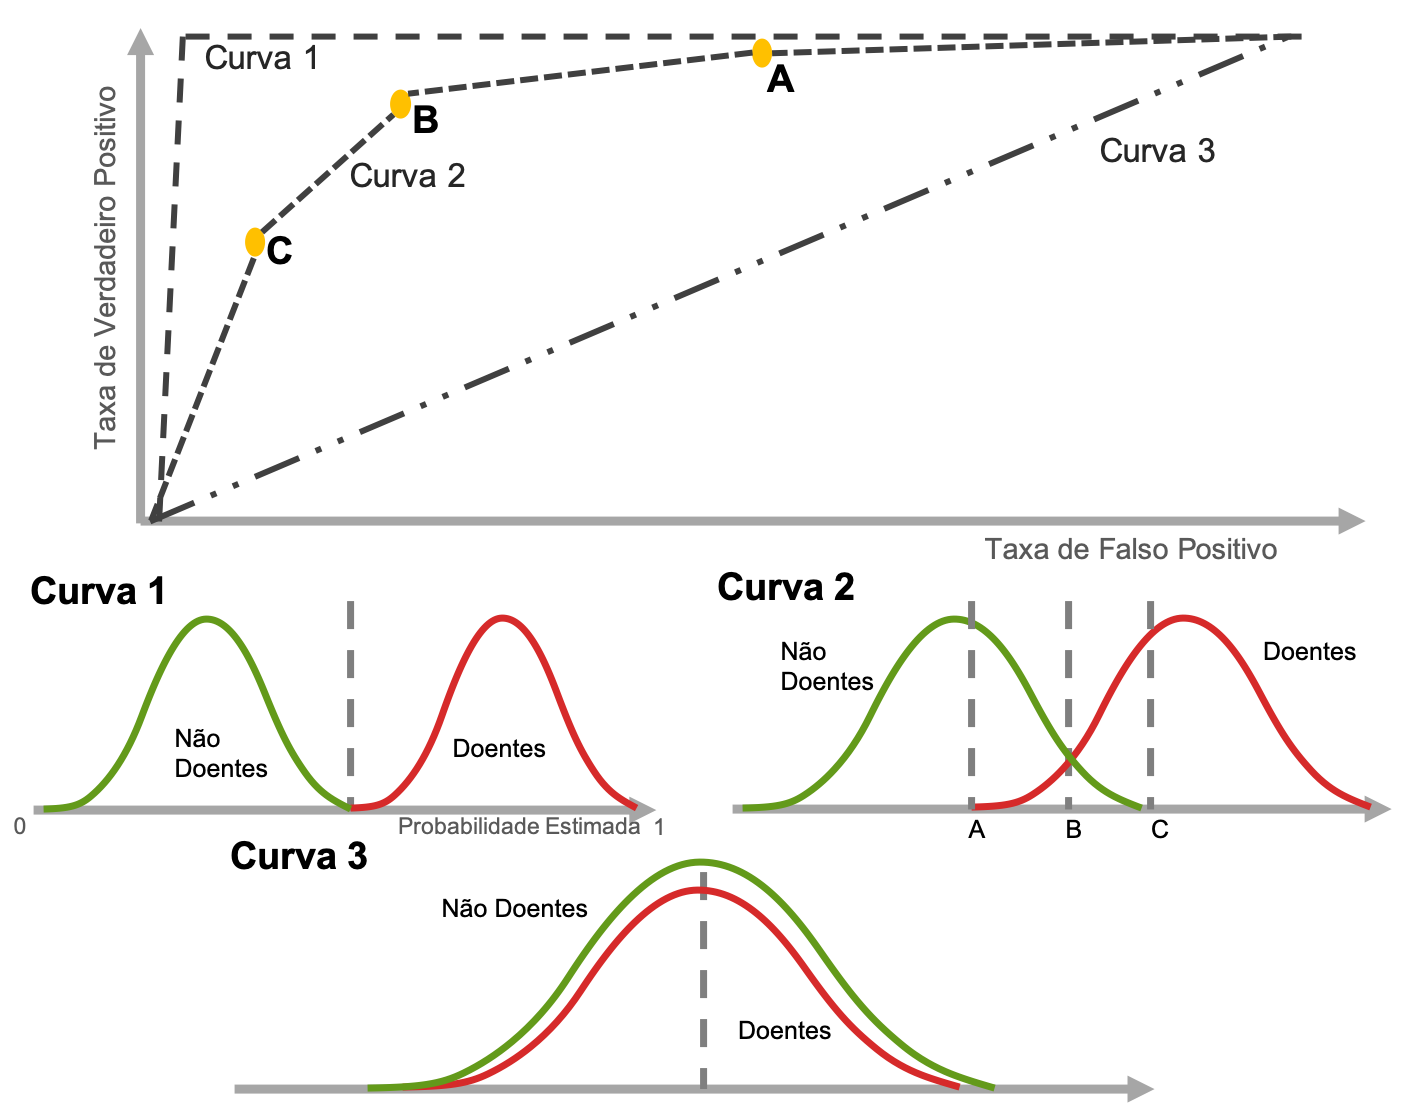
\includegraphics[width=0.75\textwidth]{pngs/roc_curvas_todas_ref_httpscienciaenegocios.comcurva-roc-e-auc-em-machine-learning.png}
\caption{Exemplos de curvas ROC para classificadores de diferentes qualidades: quanto mais a curva se aproxima do canto superior esquerdo (maior área sob a curva, AUC), melhor a capacidade discriminativa do modelo; a diagonal corresponde a um classificador aleatório (AUC = 0,5). Um exemplo intuitivo é um teste médico que classifica pacientes como doentes ou saudáveis: a taxa de verdadeiros positivos mede a fração de doentes corretamente identificados, enquanto a taxa de falsos positivos mede a fração de saudáveis erroneamente apontados como doentes. Variar o limiar de decisão move o teste ao longo da curva, negociando a detecção de mais doentes contra um número maior de alarmes falsos. Fonte: adaptado de \emph{Ciência e Negócios}\protect\footnotemark.}
\label{fig:roc_auc}
\end{center}
\end{figure}
\footnotetext{Disponível em: \url{https://cienciaenegocios.com/curva-roc-e-auc-em-machine-learning}. Acesso em: 6 abr. 2026.}

\textbf{Curva Precisão-Sensibilidade} (\textit{Precision-Recall}) --- alternativa à curva ROC, recomendada quando a classe positiva é rara ou quando o custo dos erros é assimétrico \citep{Saito2015}. Plota a precisão contra a sensibilidade para cada limiar~$\tau$. A área sob a curva PR (AUC-PR) é mais informativa que a AUC-ROC em cenários desbalanceados, pois não é inflada por verdadeiros negativos abundantes.

Nesta dissertação, os modelos são avaliados por acurácia, precisão, sensibilidade, F1-score e AUC-ROC no conjunto de teste (Capítulo~5). Para a análise de ajuste de limiar, utilizam-se também o $F_2$-score e a curva precision-recall.

\subsection{Overfitting, underfitting e o compromisso entre viés e variância}
\label{sec:overfitting}

A identificação de \textbf{sobreajuste} (overfitting) e \textbf{subajuste} (underfitting) baseia-se na comparação do desempenho do modelo nos dados usados no treinamento versus nos dados reservados para teste ou validação \citep{geron2019maos}. Em termos intuitivos: \textbf{sobreajuste} ocorre quando o modelo "decora" os dados de treino (incluindo o ruído) e deixa de generalizar --- o erro no treino fica muito baixo, mas o erro em dados novos permanece alto. \textbf{Subajuste} ocorre quando o modelo é simples demais e não captura o padrão verdadeiro dos dados --- tanto o erro de treino quanto o de validação ficam altos. 

O erro de generalização pode ser decomposto em \textbf{viés}, \textbf{variância} e \textbf{ruído irredutível} \citep{Deisenroth2019, Levada2026}. Formalmente, para um modelo $\hat{f}$ treinado em diferentes amostras do mesmo processo gerador, o erro quadrático médio esperado em um ponto $\vec{x}$ é:
\begin{equation}
\mathbb{E}\!\left[(y - \hat{f}(\vec{x}))^2\right] = \text{Viés}^2[\hat{f}(\vec{x})] + \text{Var}[\hat{f}(\vec{x})] + \sigma^2,
\label{eq:bias_variance}
\end{equation}
onde $\text{Viés}^2[\hat{f}] = \left(\mathbb{E}[\hat{f}(\vec{x})] - f(\vec{x})\right)^2$ mede o erro sistemático do modelo (quão longe a predição média está do valor verdadeiro), $\text{Var}[\hat{f}]$ mede a sensibilidade do modelo a flutuações nos dados de treino, e $\sigma^2$ é a variância do ruído intrínseco aos dados (irredutível por qualquer modelo). Modelos muito simples tendem a alto viés (subajuste); modelos muito flexíveis tendem a alta variância (sobreajuste). O objetivo prático é encontrar um equilíbrio que minimize o erro total.

\textbf{Diagnóstico.} O sinal mais claro de sobreajuste é um erro muito baixo no treino e um erro alto no teste ou validação (não generalizou). Esse diagnóstico é feito graficamente pelas \textbf{curvas de aprendizado} (Seção~\ref{sec:curvas_aprendizado}): o sobreajuste aparece como um \textbf{gap} entre a curva de treino e a de validação, enquanto o subajuste mantém ambas próximas e em um \textbf{platô alto} de erro.

A \textbf{validação cruzada} --- detalhada na Seção~\ref{sec:validacao_modelos} --- complementa esse diagnóstico ao fornecer uma estimativa robusta do erro de generalização (média e desvio padrão sobre várias divisões dos dados), facilitando perceber quando o modelo começou a sobreajustar \citep{geron2019maos}.

\ia{Em resumo: \textbf{sobreajuste} (overfitting) significa que o modelo se ajustou demais aos dados de treino (incluindo o ruído) e perde capacidade de generalizar; soluções típicas são obter mais dados, simplificar o modelo ou usar regularização (penalizar parâmetros grandes). \textbf{Subajuste} (underfitting) significa que o modelo é simples demais e não captura o padrão dos dados; as soluções envolvem aumentar a complexidade do modelo ou enriquecer as características de entrada. Os \textbf{hiperparâmetros} (por exemplo, força da regularização, profundidade máxima das árvores) controlam esse equilíbrio e podem ser escolhidos via validação cruzada.}

A \textbf{regularização} restringe a liberdade do modelo (por exemplo, penalidade \(\ell_2\) na Regressão Logística ou limites de profundidade e número de folhas nas árvores), sendo controlada por hiperparâmetros que podem ser ajustados via validação cruzada \citep{geron2019maos}. Outras formas incluem a \textbf{parada antecipada}: interromper o treinamento quando o erro no conjunto de validação deixa de melhorar, evitando que o modelo "decore" o ruído do treino. Nesta dissertação, o foco está na penalização de pesos em modelos lineares (Ridge/Lasso) e nos critérios de parada e poda nas árvores. A regularização \(\ell_1\) e \(\ell_2\) é \textbf{sensível à escala} das variáveis de entrada: atributos em escalas maiores tendem a receber pesos menores pela penalização. Em geral, recomenda-se \textbf{padronizar} as variáveis (subtrair a média e dividir pelo desvio padrão) antes de aplicar Ridge ou Lasso. 

Na \textit{pipeline} desta dissertação, as features não são padronizadas antes de todos os treinos (Capítulo 4); a justificativa é discutida naquele capítulo.

\subsection{Curvas de aprendizado}
\label{sec:curvas_aprendizado}

As \textbf{curvas de aprendizado} mostram o desempenho do modelo (acurácia ou erro) em função do tamanho do conjunto de treino (ou do número de épocas); são a ferramenta gráfica que torna visível o equilíbrio viés--variância discutido acima e auxiliam na decisão de coletar mais dados ou alterar a complexidade do modelo.

A Figura~\ref{fig:learning_curves} ilustra o conceito com curvas de aprendizado reais de três classificadores (XGBoost, Random Forest e Árvore de Decisão) em uma tarefa de classificação. Em cada painel, a curva superior é o desempenho no \textbf{treino} e a inferior o desempenho em \textbf{validação cruzada}, ambos em função do número de amostras de treino. Dois padrões didáticos aparecem: (i)~a curva de validação \textbf{sobe} à medida que mais dados ficam disponíveis e tende a um \textbf{platô}, ponto a partir do qual coletar mais exemplos pouco acrescenta; (ii)~o \textbf{intervalo} (\textit{gap}) entre a curva de treino (quase perfeita) e a de validação mede o \textbf{sobreajuste} --- quanto maior o vão, mais o modelo decorou o treino em vez de generalizar. Um modelo bem ajustado é aquele cujas duas curvas convergem para um patamar alto com vão pequeno.

\begin{figure}[h!]
\begin{center}
	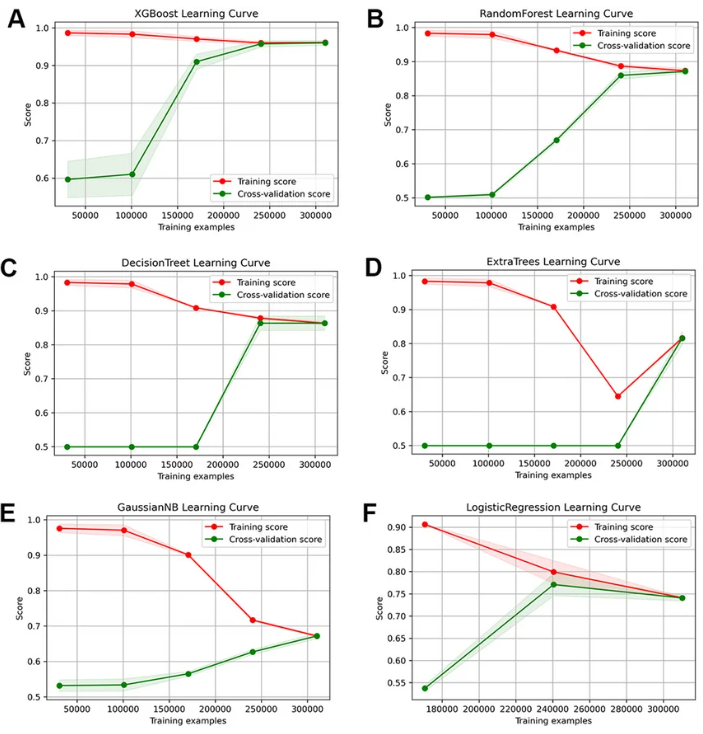
\includegraphics[width=0.8\textwidth]{pngs/Learning-curves-of-models-with-training-data-A-XGBoost-B-Random-Forest-C.png}
\caption{Exemplo de curvas de aprendizado (dados genéricos, não referentes a curvas de luz de ocultação) para três classificadores: (A)~XGBoost, (B)~Random Forest e (C)~Árvore de Decisão. Em cada painel, compara-se o desempenho no conjunto de treino com o obtido em validação cruzada, em função do número de amostras de treino; o vão entre as duas curvas indica o grau de sobreajuste, e o platô da curva de validação indica a partir de quando mais dados deixam de melhorar o modelo. Fonte: adaptado de \emph{ResearchGate}\protect\footnotemark.}
\label{fig:learning_curves}
\end{center}
\end{figure}
\footnotetext{Disponível em: \url{https://www.researchgate.net/figure/Learning-curves-of-models-with-training-data-A-XGBoost-B-Random-Forest-C_fig2_374986649}. Acesso em: 6 abr. 2026.}

\subsection{Validação de modelos}
\label{sec:validacao_modelos}

Para estimar o desempenho em dados não vistos e evitar otimismo, é essencial separar os dados usados no treino daqueles usados na avaliação \citep{geron2019maos}. Imagine que treinamos o modelo usando todas as curvas de luz disponíveis e depois o avaliamos nessas mesmas curvas. O resultado seria enganosamente bom. Para estimar honestamente o desempenho, é preciso reservar dados que o modelo nunca viu. A \textbf{validação cruzada} sistematiza esse processo: em vez de uma única divisão treino/teste (que pode ser sortuda ou azarada), roda-se o experimento $k$ vezes, cada vez deixando uma fatia diferente de fora. A média dos $k$ resultados é uma estimativa muito mais robusta do erro de generalização.

\begin{figure}[htbp]
\begin{center}
	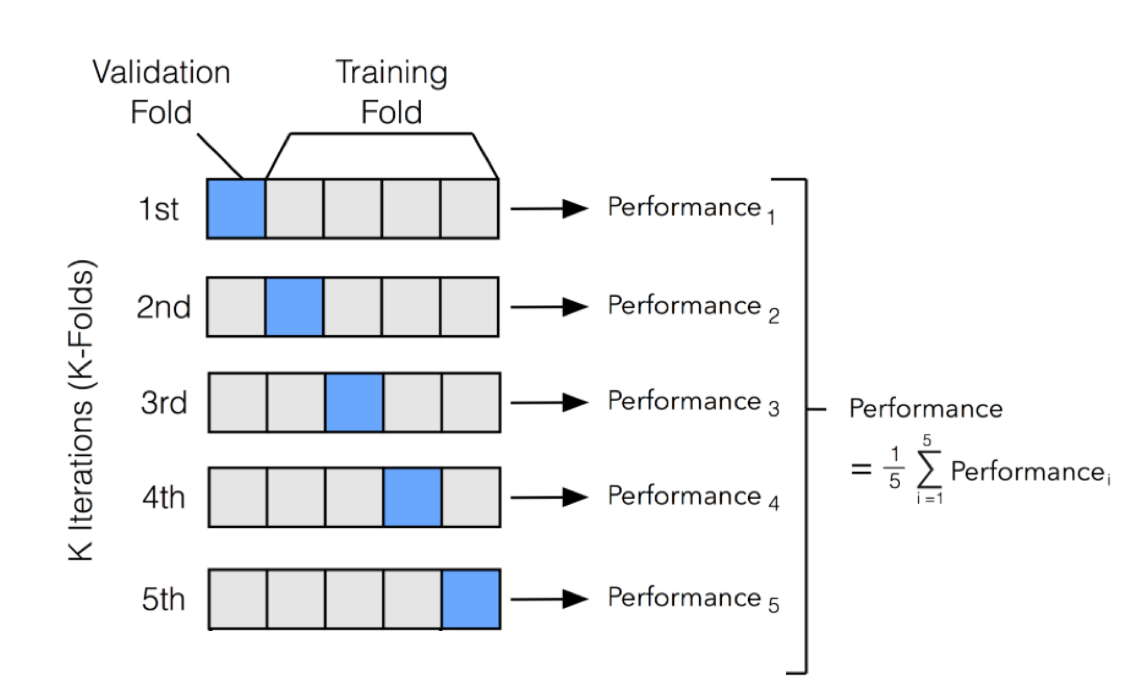
\includegraphics[width=0.75\textwidth]{pngs/kfold.png}
\caption{Esquema da validação cruzada com $k=5$: em cada rodada, uma fatia diferente (em destaque) é usada como conjunto de validação, e as demais como treino. Fonte: adaptado de Nishad~(2023)\protect\footnotemark.}
\label{fig:kfold}
\end{center}
\end{figure}
\footnotetext{Disponível em: 

\url{https://medium.com/@nishad009adi/k-fold-cross-validation-with-simple-example-e023bb2e2d43}. Acesso em: 6 abr. 2026.}

As estratégias mais comuns são:

\begin{itemize}
	\item \textbf{Conjunto de teste:} uma fração dos dados é reservada e nunca usada no treino; o desempenho nesse conjunto fornece uma estimativa do erro de generalização.
	\item \textbf{Validação cruzada (k-fold):} os dados são divididos em \(k\) partes (dobras); em cada rodada, \(k-1\) dobras são usadas para treino e uma para validação; a métrica final é a média sobre as \(k\) rodadas. Isso dá uma estimativa mais estável do desempenho e é útil para comparar modelos ou escolher hiperparâmetros (parâmetros do algoritmo que não são ajustados pelo treinamento, como a força da regularização).
	\item \textbf{Validação cruzada estratificada:} quando as classes são desbalanceadas (por exemplo, poucas curvas com ocultação e muitas sem), a divisão aleatória simples pode produzir dobras em que uma das classes está sub ou sobrerrepresentada. A validação \textbf{estratificada} preserva a proporção de cada classe em cada dobra, tornando a estimativa mais confiável \citep{geron2019maos}. Na detecção de ocultações, o uso de divisão estratificada é recomendado.
	\item \textbf{Busca em grade:} para escolher hiperparâmetros, avalia-se um conjunto de combinações (a "grade") e escolhe-se a que maximiza a métrica de validação.
\end{itemize}

Na \textit{pipeline} desta dissertação (Capítulo 4), a divisão treino/teste é feita de forma estratificada (mantendo a proporção de positivas e negativas em cada parte) ou por seleção manual de curvas para o teste. As métricas (acurácia, precisão, sensibilidade, F1-score, AUC-ROC) são calculadas no \textbf{conjunto de teste} --- dados que o modelo nunca viu durante o treinamento. \ia{Com isso, o capítulo fornece a base conceitual necessária para interpretar a metodologia e os resultados descritos no Capítulo 4.}


\chapter{Metodologia: Pipeline de Detecção}

% =============================================================================
% Capítulo 4 — Metodologia: Pré-processamento e Engenharia de Características
% =============================================================================


Este capítulo descreve a metodologia adotada para desenvolver o \textbf{fluxo de trabalho em etapas} (\textit{pipeline}) de detecção automatizada de ocultações estelares em curvas de luz. A exposição está organizada em etapas sucessivas: desde a aquisição e o armazenamento dos dados até o \textbf{treinamento} (ajuste dos parâmetros dos classificadores) e a \textbf{avaliação} (medida do desempenho em dados não usados no ajuste). 

Os objetivos deste capítulo são: (1) descrever a arquitetura completa da \textit{pipeline}, da coleta dos dados ao modelo treinado; (2) detalhar o pré-processamento das curvas de luz, incluindo fontes de dados, armazenamento em banco relacional, normalização e critérios de classificação; (3) explicar a construção do conjunto de dados utilizado no treinamento, incluindo o recorte de segmentos negativos a partir de curvas positivas e a incorporação de curvas sintéticas; (4) formalizar a engenharia de características (\textit{feature engineering}) aplicada às curvas; e (5) especificar o protocolo de treinamento e avaliação dos classificadores, com as métricas e a divisão treino/teste adotadas. Ao final, o leitor terá uma visão clara de como os dados brutos são transformados em um conjunto de atributos e como os modelos são treinados e avaliados, preparando o terreno para a discussão dos resultados no Capítulo 5.

% -----------------------------------------------------------------------------
\section{Visão geral da pipeline}
\label{sec:visao_geral}

A metodologia está organizada em uma \textit{pipeline} em etapas, na qual a saída de um bloco alimenta o seguinte. Essa estrutura facilita a manutenção, a reprodução e a extensão do trabalho. A Figura~\ref{fig:diagrama_pipeline} ilustra o fluxo desde as fontes de dados até os modelos treinados.

\textbf{Etapa 1 — Aquisição e armazenamento:} curvas de luz são obtidas a partir de portais externos (VizieR, banco do Grupo do Rio) e inseridas em um banco de dados relacional SQLite, com duas tabelas principais: \texttt{observations} (metadados da observação) e \texttt{light\_curves} (pontos tempo--fluxo).

\textbf{Etapa 2 — Acesso e normalização:} um módulo de acesso aos dados consulta o banco, filtra curvas por objeto, data e tipo (positiva ou negativa), aplica normalização do fluxo (baseline estimado por quartis) e remove \textit{outliers} quando necessário.

\textbf{Etapa 3 — Construção do conjunto de dados:} as curvas disponíveis são reunidas; segmentos sem ocultação são recortados de curvas positivas (com revisão manual) para ampliar a classe negativa; curvas sintéticas negativas são incorporadas. Em seguida, cada curva é convertida em um vetor de características (lista de números que a descrevem), formando uma tabela em que cada linha é uma curva e cada coluna é uma dessas grandezas.

\textbf{Etapa 4 — Extração de características:} para cada curva (série tempo--fluxo), são calculadas estatísticas e medidas derivadas (suavização, derivadas, comparações entre quartis, etc.), gerando a tabela de vetores da etapa 3. O Capítulo 3 já introduziu a ideia de \textit{features}; aqui detalhamos quais grandezas são extraídas.

\textbf{Etapa 5 — Treinamento e avaliação:} o conjunto de dados final é dividido em \textbf{treino} (usado para ajustar os parâmetros dos classificadores) e \textbf{teste} (reservado para medir o desempenho). Os quatro classificadores são treinados na parte de treino; o desempenho é avaliado na parte de teste (acurácia, precisão, sensibilidade, F1-score, AUC-ROC). Os modelos ajustados e os resultados são salvos em disco para análise posterior.

As seções seguintes detalham cada uma dessas etapas.

\begin{figure}[htbp]
\begin{center}
	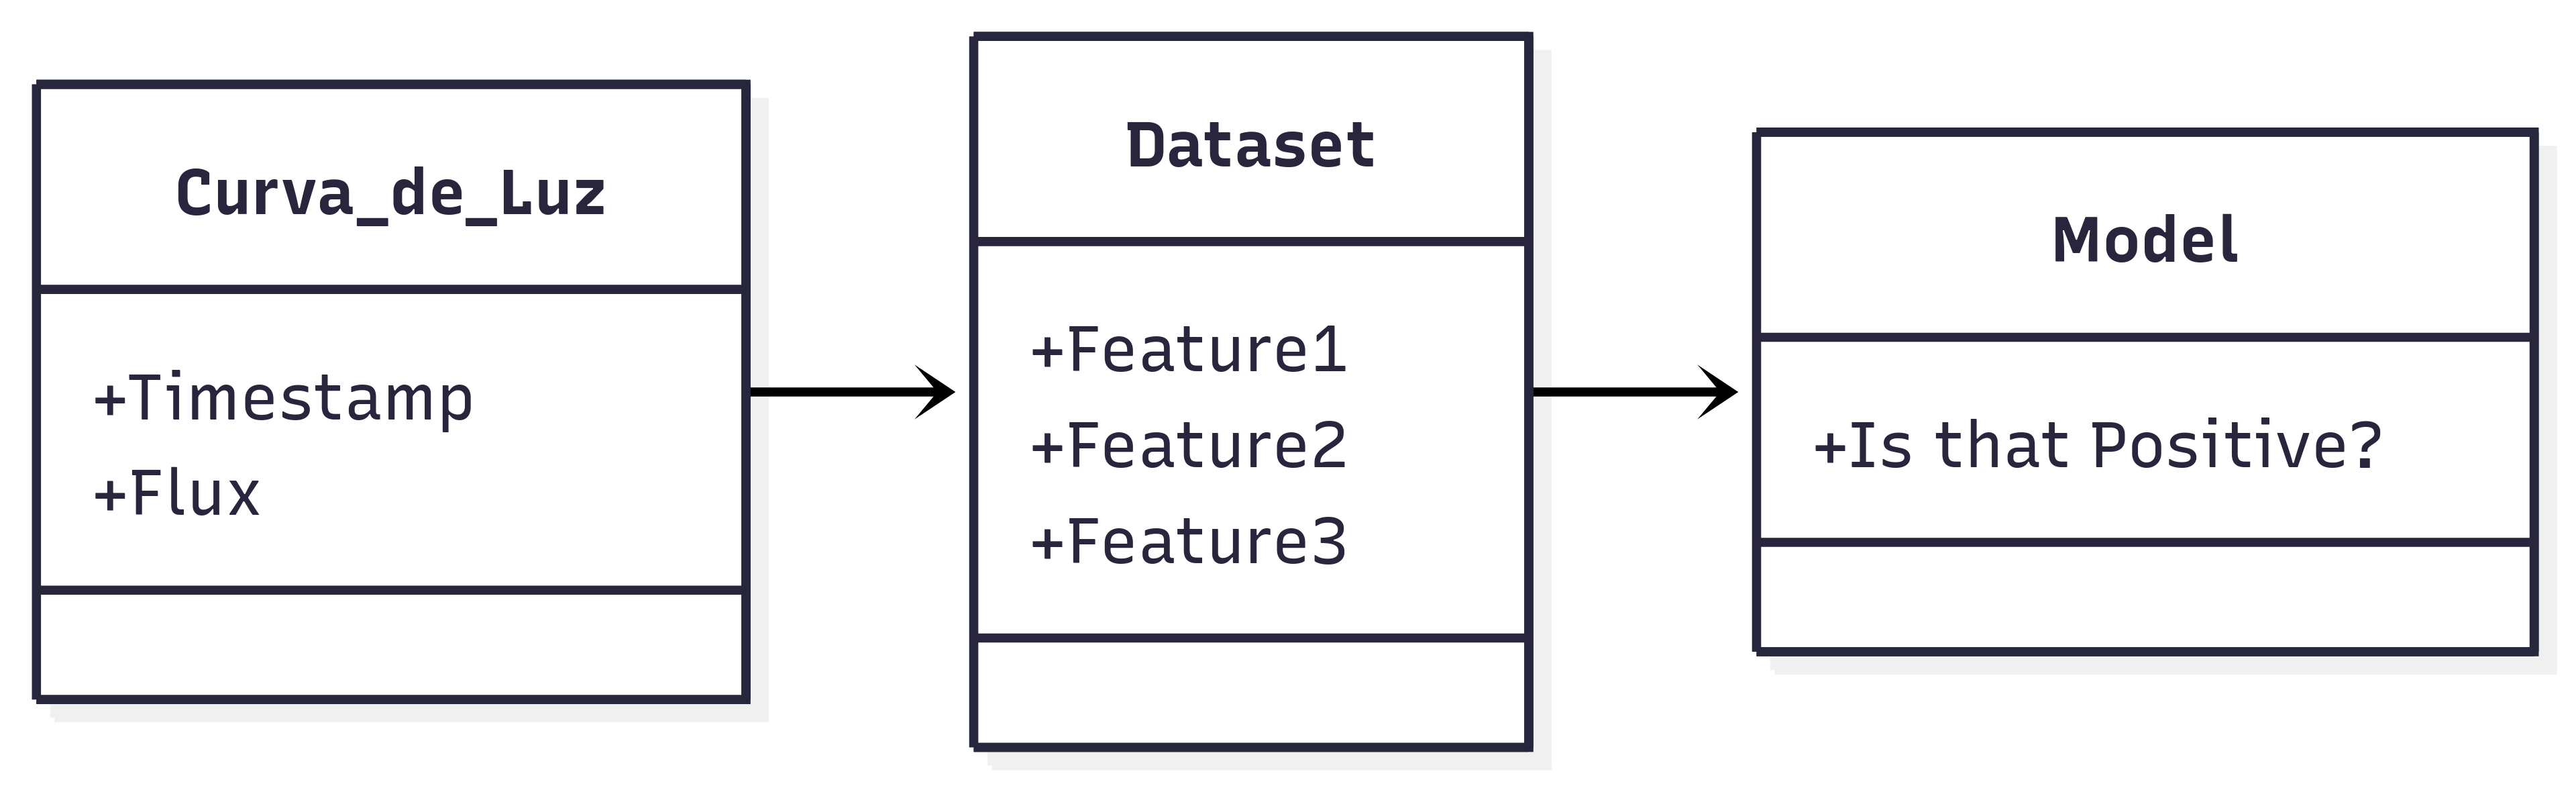
\includegraphics[scale=0.08]{pngs/diagrama_1.png}
\caption{Esquema da \textit{pipeline}: as curvas de luz são convertidas em vetores de características; o treinamento utiliza essas características, e não as séries temporais brutas.}
\label{fig:diagrama_pipeline}
\end{center}
\end{figure}

% -----------------------------------------------------------------------------
\section{Aquisição e armazenamento dos dados}
\label{sec:aquisição}

\subsection{Fontes de dados}

As curvas de luz utilizadas neste trabalho provêm de duas origens principais.

\textbf{Grupo do Rio:} parte do conjunto foi obtida a partir do banco de dados em nuvem do Grupo do Rio, referente a campanhas de ocultações já analisadas na literatura: ocultação por Umbriel (satélite de Urano), observada em 2020 e analisada por \cite{Umbriel2020}, e ocultação por Chiron, observada em 2023 e analisada por \cite{Chiron2023}. Esses dados já possuem classificação (positiva ou negativa) e metadados consistentes. 

\textbf{VizieR:} a maior parte das curvas foi adquirida no portal VizieR (\textit{cdsarc.cds.unistra.fr}), catálogo \texttt{B/occ/asteroid}, totalizando centenas de curvas em formato \texttt{.dat}, contendo séries temporais de tempo e fluxo. Para cada entrada do catálogo, os pontos da curva são baixados via serviço \texttt{vizgraph} e armazenados localmente. Convém esclarecer uma possível confusão de escalas: os milhares de registros mencionados na Introdução referem-se às \textbf{imagens (quadros)} que cada observação produz, das quais se extrai \emph{uma} curva de luz por fotometria. O conjunto de dados deste trabalho é contado em \textbf{curvas}, não em quadros --- são centenas de curvas, que, somadas aos negativos artificiais e sintéticos, totalizam as 1693 amostras detalhadas na Seção~\ref{sec:config_experimental} (Capítulo~5).

O processamento e a integração dos dados foram realizados com as bibliotecas \texttt{Astropy} e \texttt{Astroquery} (leitura e consulta a catálogos astronômicos), \texttt{asyncio} e \texttt{aiohttp} (coleta assíncrona, reduzindo o tempo total de aquisição), e \texttt{Pandas} (manipulação tabular). Scripts em Python foram desenvolvidos para automatizar a busca, o download e a organização dos arquivos.

\begin{figure}[htbp]
\begin{center}
	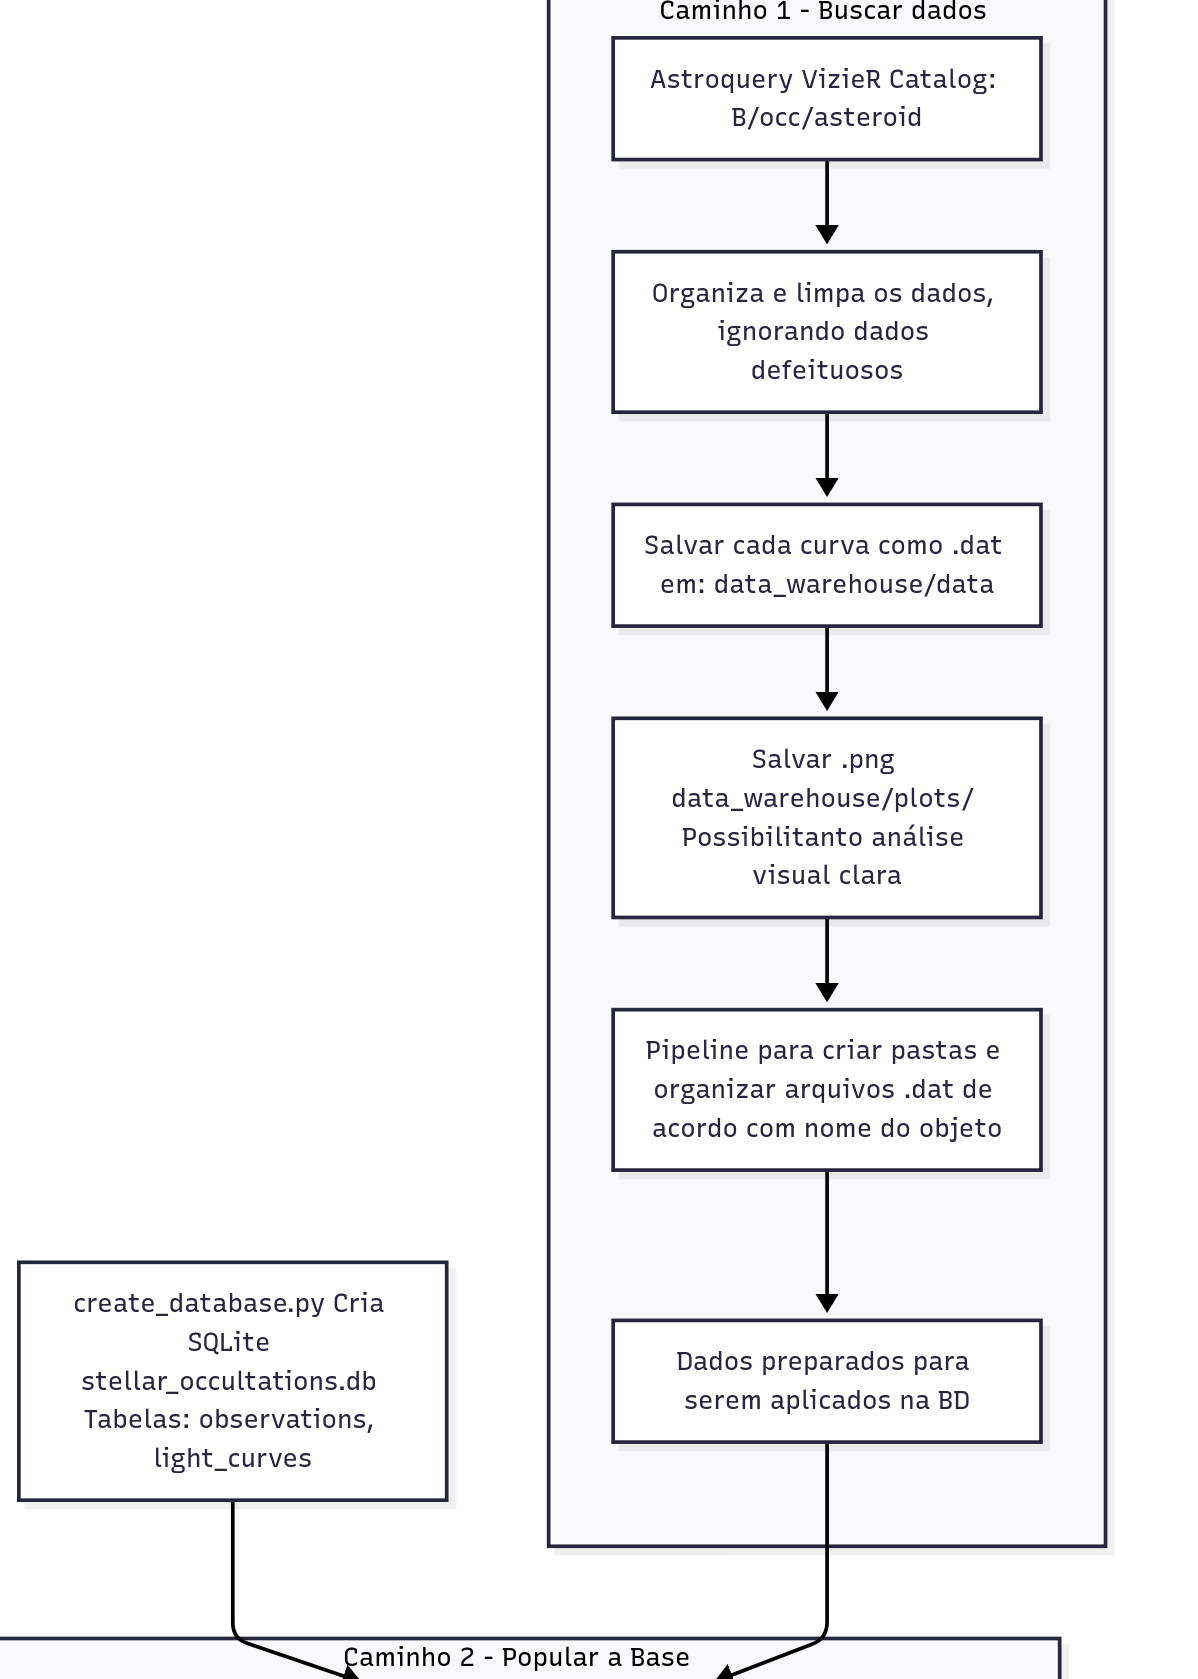
\includegraphics[scale=0.3]{pngs/fluxo1.png}
\caption{Fluxograma da aquisição e organização dos dados externos e da integração na etapa de inserção no banco de dados.}
\label{fig:fluxo1}
\end{center}
\end{figure}

\subsection{Estrutura do banco de dados}

O banco de dados relacional foi implementado em SQLite (\texttt{.db}) e estruturado em duas tabelas principais, garantindo integridade referencial e consultas eficientes.

\textbf{Tabela \texttt{observations}:} armazena informações gerais de cada observação: identificador único, nome do objeto ocultador, data da observação, portal de origem, nome do observador e metadados adicionais (incluindo a classificação do evento como ocultação positiva ou negativa, quando disponível).

\textbf{Tabela \texttt{light\_curves}:} contém os pontos individuais de cada curva de luz (tempo e fluxo), vinculados à observação correspondente por uma chave estrangeira (\texttt{observation\_id}). Assim, uma mesma observação pode possuir muitos pontos, mantendo a normalização do esquema.

Durante a inserção, buscou-se preservar ao máximo os valores originais, realizando apenas ajustes mínimos de consistência: uniformização de unidades quando necessário, checagem do alinhamento temporal e validação de metadados, sem alterar as características intrínsecas das curvas. A Figura~\ref{fig:fluxo2} resume o fluxo de consolidação do banco.

\begin{figure}[htbp]
\begin{center}
	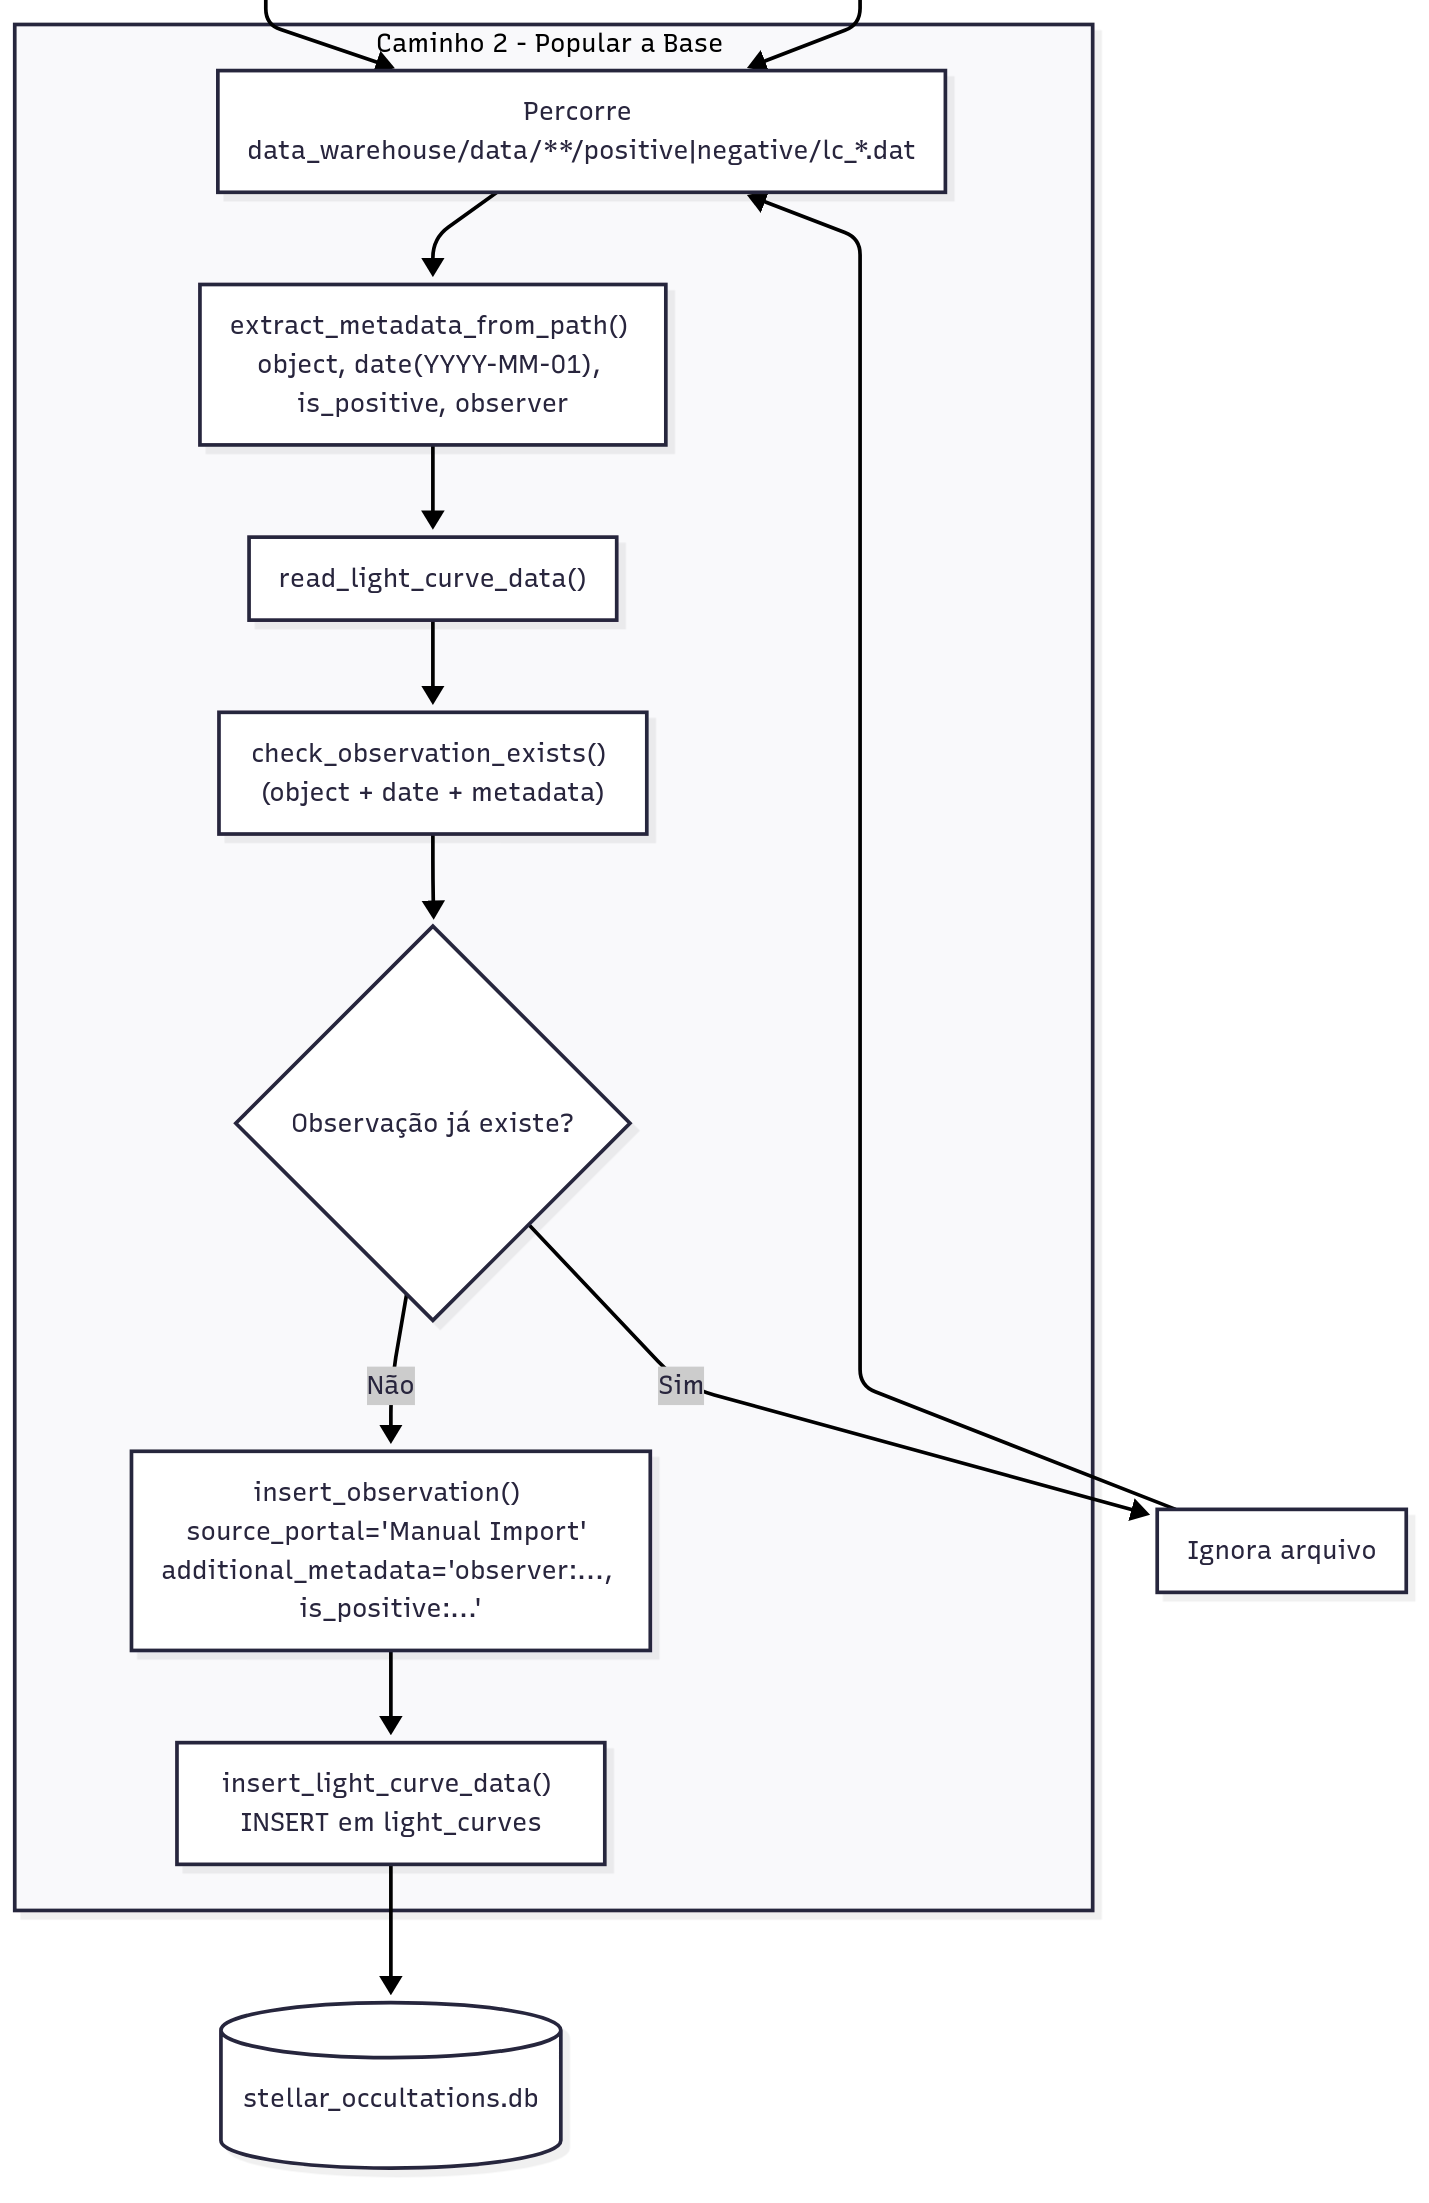
\includegraphics[scale=0.3]{pngs/fluxo2.png}
\caption{Fluxograma da \textit{pipeline} responsável pela consolidação do banco de dados.}
\label{fig:fluxo2}
\end{center}
\end{figure}

% -----------------------------------------------------------------------------
\section{Acesso aos dados e normalização}
\label{sec:acesso}

Após a consolidação no banco, um módulo dedicado (\textit{data access}) é responsável por consultar as curvas, filtrá-las por critérios (objeto, data, tipo positivo/negativo) e prepará-las para as etapas seguintes.

\subsection{Consulta e classificação}

As curvas são identificadas como \textbf{positivas} (com evento de ocultação) ou \textbf{negativas} (sem evento) com base em metadados armazenados na tabela \texttt{observations} (campo de metadados adicionais). Essa classificação pode provir de análises prévias (como no caso do Grupo do Rio) ou de anotações inseridas durante a organização dos dados. No Grupo do Rio, os rótulos decorrem das análises publicadas nas campanhas citadas (Umbriel, Chiron), realizadas por especialistas do grupo; no VizieR, a classificação positiva/negativa provém dos curadores do catálogo \texttt{B/occ/asteroid}. Não há estudo formal de concordância entre anotadores neste trabalho; as métricas de desempenho reportadas no Capítulo 5 são, portanto, relativas a esse \textit{ground truth} e devem ser lidas com a ressalva de que erros ou inconsistências de rotulagem nos catálogos podem afetar tanto o treinamento quanto a avaliação dos modelos. Durante a organização dos dados não foram identificados casos confirmados de rótulo invertido (positiva rotulada como negativa ou vice-versa); contudo, como não se realizou uma reanálise independente de cada curva, não é possível descartar a existência de inconsistências pontuais herdadas dos catálogos de origem. O módulo de acesso permite listar objetos disponíveis, datas de observação por objeto e, para cada par objeto--data, recuperar as curvas com seus rótulos.

\subsection{Normalização do fluxo}

O fluxo fotométrico bruto varia em escala entre observações (diferentes telescópios, condições de céu, etc.). Para colocar todas as curvas em uma base comparável, aplica-se uma normalização que estima um \textit{baseline} (nível de fluxo fora da ocultação) e divide-se a série pelo valor desse baseline.

A estratégia adotada é a seguinte: a série temporal do fluxo é dividida em quatro segmentos contíguos (quartis em ordem temporal). Calcula-se a média de cada segmento; os dois segmentos com maior média são considerados representativos do nível fora da ocultação. O \textit{baseline} é definido como a média dessas duas médias. O fluxo inteiro é então dividido por esse baseline, de modo que, em curvas sem ocultação ou nos trechos externos à ocultação, o valor normalizado fique próximo de 1. Em curvas com ocultação, a região de queda aparece com valores inferiores a 1. Em casos degenerados (poucos pontos ou baseline inválido), recorre-se à média global do fluxo como alternativa. A normalização coloca todas as curvas em uma escala comparável, facilitando a convergência dos algoritmos e a interpretação de resíduos; em modelos de regressão, a análise de resíduos é um diagnóstico fundamental para verificar a aderência do modelo aos dados \citep{Morettin2010}. Esse procedimento é análogo a uma normalização ``pós-fotometria'', em que o nível de continuum já foi tratado.

\subsection{Remoção de \textit{outliers}}

Quando necessário, pontos extremos do fluxo podem ser removidos com base em um critério de z-score: para um limiar \(z_{\mathrm{lim}}\) (por exemplo, 3), pontos cujo fluxo se afasta da média da série por mais de \(z_{\mathrm{lim}}\) desvios padrão são descartados. Isso reduz o impacto de picos ou quedas espúrias pontuais (defeitos de leitura, raios cósmicos, etc.) sem alterar a estrutura geral da curva.

% -----------------------------------------------------------------------------
\section{Construção do conjunto de dados para aprendizado de máquina}
\label{sec:construção_dataset}

O \textbf{conjunto de dados} (dataset) é a tabela de exemplos (curvas de luz convertidas em vetores de características) com suas classificação verdadeira (positiva ou negativa), usada para treinar e avaliar os classificadores. Devido à escassez de curvas negativas nos catálogos disponíveis, adotaram-se duas estratégias complementares: recorte de segmentos sem ocultação a partir de curvas positivas e geração de curvas sintéticas negativas com o simulador físico de Gomes-Ferrante \& Braga-Ribas~\citep{Simulator}. Os detalhes de cada estratégia são descritos nas subseções seguintes.

\subsection{Tamanho e composição do conjunto de dados}

Para interpretar sobreajuste, significância das métricas e generalização no Capítulo 5, é essencial conhecer o tamanho e a composição do conjunto utilizado. A composição final (quantidade de curvas positivas, negativas do banco, negativos artificiais por recorte manual, curvas sintéticas, total de amostras e proporção treino/teste) é apresentada na Seção 5.2 (Configuração experimental), onde os números dos experimentos são detalhados junto com a distribuição por fonte.

\subsection{Curvas positivas e negativas do banco}

As curvas classificadas como positivas são obtidas do banco via consultas que filtram observações com rótulo correspondente. As curvas negativas são obtidas da mesma forma. O número de curvas negativas ``nativas'' (observações realmente sem ocultação) costuma ser menor que o de positivas em muitos catálogos; daí a necessidade de estratégias complementares para ampliar a classe negativa.

\subsection{Recorte de segmentos negativos a partir de curvas positivas}

Uma forma de obter exemplos negativos de alta qualidade é recortar, das próprias curvas positivas, os trechos \textbf{fora} da região de ocultação (antes da imersão e depois da emersão). Esses segmentos representam o mesmo tipo de sinal (mesmo telescópio, mesma estrela, mesma noite) sem o evento, e portanto são bons candidatos a negativos.

O procedimento adotado foi o seguinte: para cada curva positiva, identifica-se a região de ocultação (por exemplo, pontos com fluxo normalizado abaixo de um limiar, e.g.\ 0,78). Os segmentos antes e depois dessa região são candidatos a negativos. Cada segmento é apresentado ao operador para revisão manual: aceitar (incorporar como negativo artificial) ou rejeitar. Quando um ou mais segmentos de uma curva positiva são aceitos, a curva positiva original é excluída do conjunto de positivos usados no treino, para evitar que a mesma observação apareça tanto como positiva quanto como negativa (vazamento de informação). Essa abordagem, embora mais trabalhosa que um recorte totalmente automático, reduz o risco de viés e garante que os negativos artificiais correspondam de fato a trechos sem ocultação.

\subsection{Curvas sintéticas negativas}

Para diversificar ainda mais a classe negativa e cobrir condições variadas de ruído e amostragem, foram incorporadas \textbf{curvas de luz sintéticas} geradas por um simulador físico. O simulador combina: (i)~geometria do evento (tempo, posição ao longo da corda); (ii)~difração de Fresnel nas bordas de imersão e emersão; (iii)~modelo de ruído (Poisson, ruído de leitura, cintilação atmosférica); (iv)~normalização pós-fotometria. Para a classe negativa, são geradas curvas sem evento (ou com diâmetro efetivo nulo), submetidas ao mesmo tipo de ruído e normalização das curvas reais. As curvas sintéticas são exportadas em formato \texttt{.dat} e carregadas pelo módulo de construção do dataset, sendo tratadas como negativas. Essa etapa permite aumentar o tamanho e a variedade do conjunto de treino e melhorar a generalização do modelo em condições diversas \citep{Simulator}.

O conjunto final reúne, portanto: positivas do banco (excluindo as usadas para recorte), negativas do banco, negativos artificiais (segmentos recortados e aprovados) e curvas sintéticas negativas. Cabe destacar que o catálogo \texttt{B/occ/asteroid} do VizieR, principal fonte das curvas positivas, é um agregador público de campanhas independentes envolvendo diferentes corpos, observadores, telescópios, datas e localizações geográficas; a diversidade observacional do conjunto positivo é, portanto, intrínseca à natureza do catálogo, e não há fonte observacional única que possa enviesar essa classe. Os pontos onde existe acoplamento entre amostras são explicitamente assumidos e mitigados: (i)~os negativos artificiais herdam telescópio, estrela e noite da curva positiva da qual foram recortados, motivo pelo qual a positiva original é excluída do conjunto de treino; (ii)~as curvas sintéticas, geradas por simulador físico, podem apresentar características de ruído distintas das observações reais, limitação retomada e quantificada no Experimento~3 (Capítulo~5). Todas as curvas passam pela mesma etapa de extração de características, descrita na próxima seção.

% -----------------------------------------------------------------------------
\section{Engenharia de características}
\label{sec:features}

As curvas de luz são séries temporais (tempo \(\times\) fluxo). Os modelos de classificação utilizados neste trabalho (Regressão Logística, Random Forest, XGBoost, CatBoost) recebem \textbf{vetores numéricos}, não as séries brutas. Por isso, cada curva é convertida em um vetor de \textbf{características} (features) extraídas da série --- por exemplo, amplitude, mínimo do fluxo suavizado, distância entre centróides do K-means, etc. O resultado é uma tabela em que cada linha é uma curva e cada coluna é uma dessas grandezas. As características foram padronizadas (média zero, desvio unitário) \textbf{apenas para a Regressão Logística}, via \texttt{StandardScaler} --- o transformador da biblioteca \texttt{scikit-learn} \citep{ScikitLearn2011} que, para cada variável, subtrai a média e divide pelo desvio padrão do conjunto de treino ---, uma vez que a regularização $\ell_2$ é sensível à escala das variáveis \citep{geron2019maos}. Os modelos baseados em árvores (Random Forest, XGBoost, CatBoost) recebem as \textit{features} em escala original, pois são insensíveis a transformações monotônicas de cada variável.

\subsection{Estatísticas básicas do fluxo}

Seja \(F(t)\) a série de fluxo (preferencialmente normalizado) com \(N\) pontos. Definem-se:

\begin{equation}
\mu = \frac{1}{N} \sum_{i=1}^{N} F(t_i), \qquad
\sigma = \sqrt{\frac{1}{N - 1} \sum_{i=1}^{N} \left( F(t_i) - \mu \right)^2},
\end{equation}

\begin{equation}
F_{\min} = \min_{1 \leq i \leq N} F(t_i), \qquad
F_{\max} = \max_{1 \leq i \leq N} F(t_i).
\end{equation}

A amplitude da curva é \(\mathrm{Amp} = F_{\max} - F_{\min}\). Em curvas com ocultação, a amplitude tende a ser maior (queda pronunciada); em curvas apenas ruidosas, \(\sigma\) e a amplitude podem ser menores. O desvio padrão \(\sigma\) e a amplitude são portanto candidatos naturais a \textit{features} discriminativas.

\subsection{Suavização e médias móveis}

Para reduzir o ruído de alta frequência sem perder a forma geral da curva, aplica-se uma janela de suavização. A suavização atua como um filtro passa-baixa: atenua as flutuações rápidas ponto a ponto (componentes de alta frequência, associadas ao ruído) e preserva as variações lentas (baixa frequência), que descrevem a forma da ocultação. A janela é adaptativa ao tamanho da série: utiliza-se \(N/40\) para séries longas (ex.: \(N > 120\) pontos) e \(N/3\) para séries mais curtas, com mínimo de 3 pontos e ímpar para filtros simétricos. Com essa janela, calculam-se:

\begin{itemize}
	\item Média móvel do fluxo; extraem-se o máximo e o mínimo da série suavizada.
	\item Filtro de Savitzky-Golay (polinômio de ordem 2), que preserva melhor os picos e vales; do fluxo suavizado por Savitzky-Golay extraem-se máximo, mínimo e desvio padrão.
\end{itemize}

Essas medidas resumem o comportamento ``suave'' da curva e são menos sensíveis a flutuações pontuais.

\subsection{Max drawdown}

O \textit{max drawdown} é a maior queda do fluxo em relação ao máximo acumulado até cada instante:

\begin{equation}
\mathrm{drawdown}(i) = F(t_i) - \max_{1 \leq j \leq i} F(t_j), \qquad
\mathrm{Max\_Drawdown} = \min_i \, \mathrm{drawdown}(i).
\end{equation}

Em curvas com ocultação, o max drawdown tende a ser mais negativo; em curvas sem evento, permanece próximo de zero (apenas flutuações).

\subsection{K-means no fluxo suavizado}

Conforme definido na Seção~\ref{sec:kmeans} (Capítulo~3), o K-means é um algoritmo de agrupamento não supervisionado; nesta etapa, ele é empregado não como classificador, mas como \textbf{extrator de característica}. Aplica-se o K-means com \(K=2\) aos valores do fluxo suavizado (Savitzky-Golay), tratando cada ponto como um vetor unidimensional. A escolha de \(K=2\) é motivada pela física do problema: espera-se que uma curva com ocultação apresente dois regimes de fluxo --- o nível fora do evento (\textit{baseline}) e o nível rebaixado durante a queda. A \textbf{distância entre os dois centróides} resultantes é então usada como \textit{feature}: curvas com ocultação bem definida tendem a apresentar distância maior; curvas apenas ruidosas, distância menor.

\subsection{Derivadas}

A partir do fluxo suavizado, calculam-se a primeira e a segunda derivada (numericamente, e.g.\ via \texttt{np.gradient}). Uma ocultação típica produz picos negativos na primeira derivada (queda) e inflexões na segunda. São extraídas estatísticas dessas derivadas: mínimo, máximo, média, desvio padrão, assimetria (\textit{skewness}) e curtose da primeira derivada; mínimo, máximo e desvio padrão da segunda derivada. Essas \textit{features} capturam a ``forma'' da transição e ajudam a distinguir quedas reais de quedas espúrias ou ruidosas.

\subsection{Comparação entre quartis (testes estatísticos)}

A série é dividida em quatro quartis temporais. Para cada par de quartis, aplicam-se um teste \(t\) de Welch (diferença de médias) e um teste de Kolmogorov-Smirnov (K-S), que compara as funções de distribuição acumulada das duas amostras e fornece um \(p\)-valor sob a hipótese de que as distribuições são iguais \citep{Wall2003, Morettin2010}. Em curvas com ocultação, pelo menos um quartil (o que contém a queda) tende a diferir dos demais; os \(p\)-valores dos testes tendem a ser pequenos. Define-se então a \textit{feature} como o menor \(p\)-valor entre todos os pares, em escala logarítmica: \(-\log_{10}(p_{\min} + \epsilon)\), para evitar \(\log(0)\). Valores altos indicam forte evidência de diferença entre segmentos, compatível com a presença de um evento.

\subsection{Métricas de profundidade, duração e ajuste de modelos}

Além das \textit{features} descritas até aqui, a \textit{pipeline} incorpora um conjunto de métricas inspiradas em critérios observacionais discutidos em fóruns entre astrônomos amadores para análise de curvas difíceis de ocultação. Não há documento oficial que defina essas grandezas como critério definitivo para classificar uma curva como positiva; no texto referimo-nos a elas simplesmente como \textbf{métricas de profundidade, duração e ajuste de modelos}, isto é, grandezas adotadas neste trabalho e inspiradas em critérios práticos de análise, sem alegar que constituam definições formais consagradas na literatura. A implementação concreta segue o módulo de engenharia de características do projeto (arquivo \texttt{occ\_features.py}), cujas fórmulas são resumidas abaixo.

\textbf{Baseline.} O nível de fluxo fora da ocultação é estimado pela mediana da série: \(\mathrm{baseline} = \mathrm{mediana}(F)\). Em implementações alternativas pode-se usar a média dos pontos com fluxo acima da mediana. A mediana é robusta a \textit{outliers} --- valores extremos isolados, como quedas ou picos pontuais causados por raios cósmicos ou defeitos de leitura ---, que pouco a deslocam, ao contrário do que ocorreria com a média.

\textbf{Profundidade do dip.} A queda do fluxo em relação ao baseline é
\begin{equation}
\mathrm{depth} = \max\big(0,\, \mathrm{baseline} - \min_i F(t_i)\big).
\end{equation}
Em curvas sem ocultação, \(\mathrm{depth} \approx 0\); em curvas com evento, \(\mathrm{depth}\) reflete a magnitude da queda.

\textbf{Desvio do baseline.} O desvio padrão \(\sigma_{\mathrm{baseline}}\) é calculado apenas sobre os pontos com fluxo \(\geq \mathrm{baseline}\) (fora do dip). Essa grandeza estima o \textbf{ruído fotométrico fora do evento}: a dispersão natural do fluxo medido quando não há ocultação, decorrente das incertezas de medição (ruído de fótons, de leitura e de cintilação atmosférica). Usá-la como referência evita contaminar a medida de ruído com a própria queda. Se houver poucos pontos acima do baseline, usa-se o desvio padrão de toda a série.

\textbf{SNR do dip.} Neste trabalho, define-se a razão sinal-ruído da queda como o quociente entre a profundidade do \textit{dip} e o ruído estimado fora do evento:
\begin{equation}
\mathrm{SNR\_dip} = \frac{\mathrm{depth}}{\sigma_{\mathrm{baseline}}}.
\end{equation}
Valores altos indicam queda significativa em relação ao ruído, compatível com evento real.

\textbf{Sequências abaixo do baseline.} Uma \textit{sequência} (\textit{run}) é um bloco consecutivo de índices em que \(F(t_i) < \mathrm{baseline}\). Ocultações típicas produzem uma sequência longa; ruído tende a sequências curtas ou isoladas. Define-se o \textbf{número de frames na maior sequência} como a quantidade de pontos do maior bloco consecutivo abaixo do baseline.

\textbf{Duração em segundos.} A duração da maior sequência é \(\Delta t = t_{\mathrm{fim}} - t_{\mathrm{início}}\), onde \(t_{\mathrm{início}}\) e \(t_{\mathrm{fim}}\) são os instantes do primeiro e do último ponto dessa sequência. Essa grandeza está ligada à geometria do evento (tamanho do objeto, velocidade).

\textbf{Fluxo mínimo e razão.} Sejam \(F_{\min} = \min_i F(t_i)\) e a razão \(F_{\min}/\mathrm{baseline}\) (quando \(\mathrm{baseline} > 0\)). Em curvas normalizadas com ocultação, a razão tende a ser menor que 1.

\textbf{Chi² do modelo constante.} O modelo ``sem evento'' assume fluxo constante igual ao baseline. Define-se
\begin{equation}
\chi^2_{\mathrm{const}} = \sum_i \frac{(F_i - \mu)^2}{\sigma^2},
\end{equation}
com \(\mu = \mathrm{baseline}\) e \(\sigma\) uma escala robusta dos resíduos (por exemplo, MAD --- mediana do valor absoluto dos desvios em relação à mediana).

\textbf{Chi² do modelo ``square well''.} O modelo com dip assume nível constante fora da janela da maior sequência e nível constante (média do fluxo) dentro da janela, em formato de ``poço retangular''. A predição \(\mathrm{pred}_i\) vale \(\mathrm{baseline}\) fora da janela e a média do fluxo na janela dentro dela. Define-se
\begin{equation}
\chi^2_{\mathrm{sw}} = \sum_i \frac{(F_i - \mathrm{pred}_i)^2}{\sigma^2}.
\end{equation}

\textbf{Razão chi².} A grandeza
\begin{equation}
\chi^2_{\mathrm{ratio}} = \frac{\chi^2_{\mathrm{const}}}{\chi^2_{\mathrm{sw}}}
\end{equation}
mede o ganho de ajuste ao incluir o dip: valores \(\chi^2_{\mathrm{ratio}} > 1\) indicam que o modelo com dip explica melhor os dados. Na implementação, a razão é limitada ao intervalo \([0{,}1,\, 10]\) para evitar valores extremos. Curvas sem dip tendem a \(\chi^2_{\mathrm{ratio}} \approx 1\).

No dataset gerado pela \textit{pipeline}, essas grandezas aparecem em colunas cujos nomes no código possuem o prefixo \texttt{Occ\_} (de \textit{occultation}), por exemplo \texttt{Occ\_depth}, \texttt{Occ\_duration\_s}. No texto, tratamos todas elas como métricas de profundidade, duração e ajuste de modelos.

\subsection{Resumo das \textit{features}}

O vetor final de \textit{features} inclui: amplitude e desvio padrão do fluxo; máximo e mínimo da média móvel e do Savitzky-Golay; max drawdown; distância entre centróides do K-means no fluxo; mínimos \(-\log_{10}(p)\) dos testes \(t\) e K-S entre quartis; as estatísticas das derivadas primeira e segunda listadas acima; e as métricas de profundidade, duração e ajuste de modelos (profundidade do dip, SNR do dip, duração em segundos da maior sequência abaixo do baseline, número de frames na maior sequência, desvio padrão do baseline, fluxo mínimo, razão fluxo mínimo/baseline, \(\chi^2\) do modelo constante, \(\chi^2\) do modelo square well, razão \(\chi^2_{\mathrm{const}}/\chi^2_{\mathrm{sw}}\)). Todas as colunas de \textit{features} são numéricas; metadados como identificador da curva e rótulo (positivo/negativo) são mantidos em colunas separadas e não são usados como entrada do classificador. O resultado da etapa de engenharia de características é um arquivo tabular (por exemplo, \texttt{dataset\_final.csv}) em que cada linha é uma curva e as colunas são as \textit{features} mais o rótulo e o identificador.

% -----------------------------------------------------------------------------
\section{Treinamento e avaliação dos modelos}
\label{sec:treinamento}

\subsection{Preparação dos dados e divisão treino/teste}

O dataset final é carregado a partir do arquivo gerado na etapa anterior. As colunas de metadados (identificador da curva, fonte, rótulo) são separadas das colunas de \textit{features}. Valores faltantes (NaN) são preenchidos pela \textbf{mediana} calculada no conjunto de treino (\texttt{SimpleImputer} com \texttt{strategy='median'}), estratégia robusta a \textit{outliers}. O rótulo binário (ocultação presente = 1, ausente = 0) é definido como variável alvo.

A divisão entre treino e teste pode ser feita de duas formas:

\begin{enumerate}
	\item \textbf{Divisão estratificada:} os dados são divididos aleatoriamente em conjunto de treino e conjunto de teste (por exemplo, 80\% treino e 20\% teste), mantendo a proporção das classes em cada parte (\textit{stratified split}). Uma semente fixa (\textit{random state}) é utilizada na divisão para garantir reprodutibilidade; a mesma semente (ou sementes documentadas) é empregada no treinamento de cada modelo (Regressão Logística, Random Forest, XGBoost, CatBoost), de modo que os experimentos sejam reproduzíveis.
	\item \textbf{Seleção manual de teste:} um subconjunto de curvas é fixado como conjunto de teste (por exemplo, curvas de um objeto ou data específicos). O restante compõe o treino. Essa opção é útil para avaliar a generalização para cenários de interesse conhecido.
\end{enumerate}

As métricas de desempenho (acurácia, precisão, sensibilidade, F1-score, AUC-ROC) são calculadas no conjunto de teste e reportadas no Capítulo 5. Quando a escolha de hiperparâmetros for feita por validação cruzada, pode-se reportar também a média e o desvio padrão da métrica nas dobras de validação, para dar noção da variabilidade; no conjunto de teste, as métricas são reportadas como valor único, condicionado à divisão treino/teste adotada.

\subsection{Modelos utilizados}

Foram utilizados quatro algoritmos de classificação supervisionada, descritos no Capítulo 3:

\begin{itemize}
	\item \textbf{Regressão Logística:} classificador linear probabilístico com regularização \(\ell_2\) (Ridge) ou \(\ell_1\) (Lasso); hiperparâmetro de força de regularização (\(C\) ou \(\alpha\)) escolhido via validação cruzada.
	\item \textbf{Random Forest:} ensemble de árvores de decisão com \textit{bagging}; hiperparâmetros típicos incluem número de árvores (\textit{n\_estimators}), profundidade máxima (\textit{max\_depth}) e peso das classes (\textit{class\_weight='balanced'}) para lidar com desbalanceamento.
	\item \textbf{XGBoost:} \textit{gradient boosting} com árvores; controle de profundidade, taxa de aprendizado (\textit{learning\_rate}), subamostragem de linhas e colunas.
	\item \textbf{CatBoost:} outro algoritmo de \textit{boosting}, com opção de ponderação automática das classes (\textit{auto\_class\_weights='Balanced'}).
\end{itemize}

Os valores concretos dos hiperparâmetros utilizados nos experimentos (e eventual busca em grade ou validação cruzada) estão documentados no Apêndice~\ref{ap:hiperparametros}. A escolha desses modelos deve-se ao seu bom desempenho em problemas de classificação com dados tabulares, à interpretabilidade (importância de variáveis) e à disponibilidade em bibliotecas estáveis (scikit-learn, XGBoost, CatBoost). Para quantificar a interpretabilidade, a \textbf{importância das variáveis} é calculada da seguinte forma: nos ensembles baseados em árvores (Random Forest, XGBoost, CatBoost), utiliza-se a importância por \textbf{queda média na impureza} (Gini) em cada divisão em que a variável participa, conforme fornecido pelas respectivas bibliotecas; na Regressão Logística, utilizam-se os coeficientes estimados (em valor absoluto). Os rankings e as magnitudes das importâncias são apresentados e discutidos no Capítulo 5.

\subsection{Métricas de avaliação}

As definições formais das métricas de classificação binária utilizadas neste trabalho --- acurácia, precisão, sensibilidade, F1-score, $F_\beta$-score, AUC-ROC e curva precision-recall --- foram apresentadas na Seção~\ref{sec:metricas_avaliacao} (Capítulo~3). Aqui, discutem-se as escolhas específicas adotadas na \textit{pipeline} à luz do problema de detecção de ocultações.

Em problemas de detecção de eventos, a matriz de confusão e as métricas dela derivadas permitem avaliar a capacidade do modelo de tomar decisões confiáveis \citep{Cazeneuve2023}. A \textbf{curva ROC} visualiza o \textit{trade-off} entre a taxa de verdadeiros positivos (sensibilidade) e a taxa de falsos positivos à medida que o limiar de decisão varia; a \textbf{área sob a curva} (AUC-ROC) resume a capacidade de ordenação do modelo de forma independente do limiar escolhido \citep{AUC-curve}. Em problemas com \textbf{classe positiva rara} --- isto é, quando os exemplos de interesse (positivos) são minoria expressiva frente aos negativos ---, a \textbf{curva precision-recall} pode ser mais informativa, pois não é inflada pelo grande número de verdadeiros negativos.

No contexto desta dissertação, em que os dados são desbalanceados (muitas curvas sem ocultação), a \textbf{acurácia} sozinha pode ser enganosa, conforme ilustrado pelo exemplo numérico do Capítulo~3. Para detecção de ocultações estelares, a \textbf{sensibilidade} tem prioridade, pois não perder eventos raros é essencial; a \textbf{precisão} evita excesso de falsos positivos que sobrecarregariam a triagem humana. O \textbf{F1-score} equilibra precisão e sensibilidade e é adequado para comparar os quatro modelos em cenário desbalanceado. A \textbf{AUC-ROC} avalia a capacidade de separação das classes de forma global.

\subsection{Fluxo de treinamento e persistência}

O fluxo de treinamento é: (1)~carregar o conjunto de dados; (2)~separar as colunas de características das colunas de rótulo (positivo/negativo); (3)~dividir em treino e teste (por exemplo, 80\% treino, 20\% teste); (4)~treinar cada um dos quatro modelos no conjunto de treino; (5)~avaliar cada modelo no conjunto de teste, calculando as métricas acima; (6)~gerar visualizações (curvas ROC, matrizes de confusão, importância de cada variável); (7)~salvar os modelos ajustados e um resumo das métricas em disco. Os modelos salvos podem ser carregados depois para classificar novas curvas ou para comparação com outras configurações. Os resultados numéricos e as figuras são a base da discussão do Capítulo 5.

% -----------------------------------------------------------------------------
%\section{Considerações finais do capítulo}
%\label{sec:consideracoes_cap4}

Este capítulo apresentou a metodologia completa da \textit{pipeline} de detecção de ocultações estelares em curvas de luz: desde a aquisição e o armazenamento em banco relacional até o treinamento e a avaliação de classificadores. A arquitetura em etapas (aquisição \(\to\) acesso e normalização \(\to\) construção do dataset \(\to\) engenharia de características \(\to\) treinamento) permite reproduzir o fluxo e estendê-lo com novas fontes de dados, novas \textit{features} ou novos modelos. A combinação de dados reais (VizieR, Grupo do Rio), negativos artificiais obtidos por recorte manual e curvas sintéticas visa um conjunto de treino equilibrado e representativo. A extração de características baseada em estatísticas, suavização, derivadas e testes entre quartis fornece uma representação vetorial adequada aos modelos de árvore e à Regressão Logística utilizados. No próximo capítulo, são apresentados os resultados obtidos com os quatro modelos treinados (Regressão Logística, Random Forest, XGBoost, CatBoost), incluindo comparação de desempenho, análise de importância das variáveis e discussão sobre generalização e possível overfitting.


\chapter{Resultados}

% =============================================================================
% Capítulo 5 — Resultados
% =============================================================================
% Este capítulo apresenta os resultados dos experimentos de classificação
% binária para detecção de ocultações estelares em curvas de luz, em conformidade
% com a metodologia descrita no Capítulo 4.

\section{Visão geral dos experimentos}
\label{sec:visao_geral_resultados}

Este capítulo apresenta os resultados obtidos com a \textit{pipeline} de detecção automatizada de ocultações estelares em curvas de luz, descrita no Capítulo~4. O problema é formulado como \textbf{classificação binária}: cada curva é rotulada como \textbf{positiva} (evento de ocultação presente) ou \textbf{negativa} (ausência de evento). Foram treinados e avaliados quatro classificadores --- Regressão Logística, Random Forest, XGBoost e CatBoost --- cujo desempenho foi medido exclusivamente no \textbf{conjunto de teste}, isto é, em dados que não participaram do treinamento.

As métricas adotadas são: \textbf{acurácia} (fração de acertos no total), \textbf{precisão} (entre as curvas classificadas como positivas, quantas eram realmente positivas), \textbf{sensibilidade} ou \textit{recall} (entre todas as curvas realmente positivas, quantas foram detectadas), \textbf{F1-score} (média harmônica entre precisão e sensibilidade) e \textbf{área sob a curva ROC} (AUC-ROC), que resume a capacidade do modelo de separar as duas classes para diversos limiares de decisão. As \textbf{matrizes de confusão} mostram quantos verdadeiros positivos (TP), verdadeiros negativos (TN), falsos positivos (FP) e falsos negativos (FN) cada modelo produziu.

A montagem de um conjunto de dados equilibrado foi a primeira grande dificuldade do projeto: nos catálogos disponíveis (VizieR, Grupo do Rio), o número de curvas negativas é muito inferior ao de positivas --- o banco dispunha de 802 curvas positivas e apenas 3 negativas. Para contornar esse desbalanceamento, adotaram-se duas estratégias complementares, descritas no Capítulo~4: recorte de segmentos sem ocultação a partir das curvas positivas (com revisão manual), gerando 186 negativos artificiais, e incorporação de 702 curvas sintéticas negativas geradas pelo simulador físico de Gomes-Ferrante \& Braga-Ribas~\citep{Simulator}. O \textit{dataset} final reúne \textbf{1693 amostras} (802 positivas e 891 negativas), com divisão treino/teste estratificada por curva (80\%/20\%).

Ao todo, foram realizados \textbf{seis experimentos}, que variam o conjunto de \textit{features} (de 28 a 11 variáveis) e a composição do conjunto de teste (misto ou exclusivamente real). Como o desempenho se mostrou notavelmente estável entre eles, este capítulo apresenta \textbf{em detalhe os três experimentos mais informativos}, que sintetizam a progressão lógica do trabalho:

\begin{itemize}
	\item \textbf{Experimento 1:} conjunto completo de 28 \textit{features}, divisão 80\%/20\%. É a \textbf{linha de base} de desempenho, com todas as variáveis disponíveis.
	\item \textbf{Experimento 2:} 11 \textit{features} (sem \texttt{Feature\_Savgol\_Min} e sem \texttt{kmeans\_centroid\_dist}), divisão 80\%/20\%. É a \textbf{configuração enxuta} adotada como referência operacional --- a mais simples sem perda de desempenho, e a usada no estudo de caso de Quaoar.
	\item \textbf{Experimento 3:} 11 \textit{features}, porém com \textbf{teste somente em curvas reais} (excluindo as sintéticas). É o teste de \textbf{generalização} mais próximo do uso real.
\end{itemize}

Os demais três experimentos --- a redução intermediária de \textit{features} para 14 (Experimento 4) e 13 variáveis (Experimento 5) e a ablação isolada da \textit{feature} \texttt{kmeans\_centroid\_dist} (Experimento 6) --- conduzem às mesmas conclusões e estão documentados em detalhe no Apêndice~\ref{ap:experimentos}. Suas métricas são consolidadas, ao lado das dos três experimentos-destaque, na Tabela~\ref{tab:comparacao_f1} (Seção~\ref{sec:comparacao}).

Em todos os experimentos, o mesmo protocolo foi aplicado: divisão treino/teste estratificada, preenchimento de valores faltantes pela mediana calculada no treino, e padronização das características (média zero, desvio unitário) apenas para a Regressão Logística, conforme detalhado no Capítulo~4.

Além dos experimentos de classificação, este capítulo apresenta uma análise de \textbf{ajuste do limiar de decisão} (Seção~\ref{sec:threshold_tuning}), que investiga como reduzir o limiar de classificação para minimizar falsos negativos --- uma demanda natural em cenários de triagem científica, onde perder uma ocultação real é mais custoso do que revisar um falso alarme. Por fim, um \textbf{estudo de caso} (Seção~\ref{sec:estudo_caso_quaoar}) aplica a \textit{pipeline} a curvas reais de uma ocultação estelar pelo objeto transnetuniano (50000) Quaoar~\citep{Quaoar2023} --- dados externos ao banco de treino e morfologicamente complexos (corpo principal e estruturas de anel) --- como teste de generalização operacional e como demonstração da capacidade de revisitar curvas em busca de eventos sutis.

% -----------------------------------------------------------------------------
\section{Descrição das \textit{features} e análise de redundância}
\label{sec:features_redundancia}

\subsection{Conjunto completo de \textit{features}}

A \textit{pipeline} de extração de características produz 28 variáveis numéricas a partir de cada curva de luz normalizada. Essas variáveis podem ser agrupadas em cinco famílias, descritas na Tabela~\ref{tab:features_completo}.

\begin{table}[htbp]
\centering
\caption{Conjunto completo de 28 \textit{features} extraídas pela \textit{pipeline}. A coluna ``Família'' indica o grupo funcional; a coluna ``Definição'' resume o cálculo.}
\label{tab:features_completo}
\footnotesize
\begin{tabular}{llp{7.5cm}}
\hline
\textbf{Família} & \textbf{Feature} & \textbf{Definição} \\
\hline
\multirow{3}{*}{Fluxo bruto}
& \texttt{Feature\_Amp} & $\max(f) - \min(f)$ (amplitude total do fluxo) \\
& \texttt{Feature\_Flux\_std} & $\sigma(f)$ (desvio padrão do fluxo) \\
& \texttt{Max\_Drawdown} & $\min(f_i - \max_{j \le i} f_j)$ (maior queda acumulada) \\
\hline
\multirow{3}{*}{Savitzky-Golay}
& \texttt{Feature\_Savgol\_Max} & $\max(\tilde{f})$ (máximo do fluxo suavizado) \\
& \texttt{Feature\_Savgol\_Min} & $\min(\tilde{f})$ (mínimo do fluxo suavizado) \\
& \texttt{Feature\_Savgol\_std} & $\sigma(\tilde{f})$ (desvio padrão do fluxo suavizado) \\
\hline
K-Means & \texttt{kmeans\_centroid\_dist} & Distância entre os 2 centróides do K-Means aplicado a $\tilde{f}$ \\
\hline
\multirow{2}{*}{Testes de quartis}
& \texttt{MinLogP\_Ttest} & $-\log_{10}(\min p_{\text{t-test}})$ entre pares de quartis \\
& \texttt{MinLogP\_KS} & $-\log_{10}(\min p_{\text{KS}})$ entre pares de quartis \\
\hline
\multirow{9}{*}{Derivadas}
& \texttt{Deriv\_Min} & $\min(f')$ \\
& \texttt{Deriv\_Max} & $\max(f')$ \\
& \texttt{Deriv\_Mean} & $\bar{f'}$ \\
& \texttt{Deriv\_Std} & $\sigma(f')$ \\
& \texttt{Deriv\_Skew} & Assimetria de $f'$ \\
& \texttt{Deriv\_Kurtosis} & Curtose de $f'$ \\
& \texttt{SecondDeriv\_Min} & $\min(f'')$ \\
& \texttt{SecondDeriv\_Max} & $\max(f'')$ \\
& \texttt{SecondDeriv\_Std} & $\sigma(f'')$ \\
\hline
\multirow{10}{*}{Observacionais}
& \texttt{Occ\_depth} & $\text{baseline} - \min(f)$ (profundidade do dip) \\
& \texttt{Occ\_SNR\_dip} & $\text{depth}/\sigma_{\text{baseline}}$ (razão sinal-ruído do dip) \\
& \texttt{Occ\_duration\_s} & Duração do maior bloco abaixo do baseline (em segundos) \\
& \texttt{Occ\_n\_frames\_below\_baseline} & Maior nº de frames consecutivos abaixo do baseline \\
& \texttt{Occ\_baseline\_std} & $\sigma(f \mid f \ge \text{baseline})$ (ruído fora do dip) \\
& \texttt{Occ\_flux\_min} & $\min(f)$ \\
& \texttt{Occ\_flux\_min\_over\_baseline} & $\min(f)/\text{baseline}$ \\
& \texttt{Occ\_chi2\_constant} & $\chi^2$ do modelo constante (sem evento) \\
& \texttt{Occ\_chi2\_square\_well} & $\chi^2$ do modelo de poço retangular \\
& \texttt{Occ\_chi2\_ratio} & $\chi^2_{\text{const}}/\chi^2_{\text{sw}}$ (razão de ajuste) \\
\hline
\end{tabular}
\end{table}

Nas definições acima, $f$ denota o vetor de fluxo normalizado, $\tilde{f}$ o fluxo suavizado por filtro Savitzky-Golay (polinômio de grau 2, janela adaptativa), $f'$ e $f''$ a primeira e segunda derivadas numéricas de $\tilde{f}$, e \emph{baseline} a mediana de $f$.

\subsection{Análise de redundância}

A presença de variáveis redundantes --- altamente correlacionadas ou conceitualmente equivalentes --- pode inflar a dimensionalidade sem acrescentar informação discriminativa, aumentar o risco de \textit{overfitting} e dificultar a interpretação da importância das \textit{features}. Para identificar pares redundantes, foram analisadas tanto as definições matemáticas quanto as correlações empíricas entre as 28 variáveis. Os pares identificados são apresentados a seguir.

\begin{enumerate}
	\item \textbf{\texttt{Feature\_Amp} vs.\ \texttt{Occ\_depth}.}
	A amplitude é definida como $\max(f) - \min(f)$, enquanto a profundidade observacional é $\text{baseline} - \min(f)$, com $\text{baseline} = \text{mediana}(f)$. Para curvas de fluxo normalizado próximo de 1, o máximo tende a coincidir com a mediana, tornando as duas métricas praticamente idênticas. \textbf{Removida:} \texttt{Feature\_Amp}. \textbf{Mantida:} \texttt{Occ\_depth}, por possuir motivação física direta na caracterização de ocultações.

	\item \textbf{\texttt{Feature\_Flux\_std} vs.\ \texttt{Occ\_baseline\_std}.}
	O desvio padrão do fluxo total ($\sigma(f)$) inclui os pontos dentro do dip, inflando a medida de ruído quando há ocultação. O desvio padrão do \textit{baseline} ($\sigma(f \mid f \ge \text{mediana})$) estima o ruído fotométrico fora do evento, sendo mais adequado fisicamente. \textbf{Removida:} \texttt{Feature\_Flux\_std}. \textbf{Mantida:} \texttt{Occ\_baseline\_std}.

	\item \textbf{\texttt{Occ\_flux\_min} vs.\ \texttt{Feature\_Savgol\_Min}.}
	O mínimo do fluxo bruto e o mínimo do fluxo suavizado por Savitzky-Golay são altamente correlacionados, pois o filtro preserva a posição dos mínimos. A versão suavizada é mais robusta a ruído pontual. \textbf{Removida:} \texttt{Occ\_flux\_min}. \textbf{Mantida:} \texttt{Feature\_Savgol\_Min}.

	\item \textbf{\texttt{Occ\_flux\_min\_over\_baseline}.}
	Esta razão ($\min(f)/\text{baseline}$) é algebricamente derivável de \texttt{Occ\_depth} e do valor do \textit{baseline}, não acrescentando informação independente. \textbf{Removida.}

	\item \textbf{\texttt{Occ\_n\_frames\_below\_baseline} vs.\ \texttt{Occ\_duration\_s}.}
	Para observações com cadência uniforme, a duração em segundos é proporcional ao número de frames ($\Delta t_{\text{dur}} \approx n_{\text{frames}} \times \delta t$). A duração em unidade física (segundos) é mais interpretável e invariante a mudanças de cadência. \textbf{Removido:} \texttt{Occ\_n\_frames\_below\_baseline}. \textbf{Mantida:} \texttt{Occ\_duration\_s}.

	\item \textbf{\texttt{Feature\_Savgol\_Max}.}
	Para fluxo normalizado, o máximo do sinal suavizado é próximo de 1,0 em quase todas as curvas, resultando em variância muito baixa e poder discriminativo desprezível. \textbf{Removida.}

	\item \textbf{Nove \textit{features} de derivadas (\texttt{Deriv\_*} e \texttt{SecondDeriv\_*}).}
	No Experimento 4, a remoção das nove \textit{features} de derivadas não causou perda de desempenho (F1 mantido em 0,99). Além disso, as métricas observacionais de profundidade, duração e razão $\chi^2$ já capturam as variações abruptas do fluxo que as derivadas buscam codificar, caracterizando redundância conceitual. \textbf{Removidas} todas as nove variáveis de derivadas.
\end{enumerate}

Após a remoção, o conjunto final utilizado no treinamento contém \textbf{13 \textit{features}}, listadas na Tabela~\ref{tab:features_final}.

\begin{table}[htbp]
\centering
\caption{Conjunto final de 13 \textit{features} após remoção de redundâncias.}
\label{tab:features_final}
\begin{tabular}{ll}
\hline
\textbf{Família} & \textbf{Feature} \\
\hline
Savitzky-Golay & \texttt{Feature\_Savgol\_Min}, \texttt{Feature\_Savgol\_std} \\
Fluxo bruto & \texttt{Max\_Drawdown} \\
K-Means & \texttt{kmeans\_centroid\_dist} \\
Testes de quartis & \texttt{MinLogP\_Ttest}, \texttt{MinLogP\_KS} \\
\multirow{2}{*}{Observacionais} & \texttt{Occ\_depth}, \texttt{Occ\_SNR\_dip}, \texttt{Occ\_duration\_s} \\
& \texttt{Occ\_baseline\_std}, \texttt{Occ\_chi2\_constant}, \texttt{Occ\_chi2\_square\_well}, \texttt{Occ\_chi2\_ratio} \\
\hline
\end{tabular}
\end{table}

É importante ressaltar que as 15 variáveis removidas \textbf{continuam sendo calculadas e armazenadas} no arquivo CSV do \textit{dataset}. A exclusão ocorre apenas no momento do treinamento, por meio de uma lista configurável no código (\texttt{EXCLUDED\_FEATURES}). Essa decisão de projeto permite re-incluir qualquer variável em estudos futuros de ablação sem necessidade de reprocessar as curvas de luz.

% -----------------------------------------------------------------------------
\section{Importância das \textit{features}: metodologia}
\label{sec:feature_importance_metodologia}

Uma das vantagens de modelos baseados em árvores e de modelos lineares é a possibilidade de quantificar a contribuição individual de cada variável para a decisão do classificador. Entretanto, cada família de modelos emprega uma definição distinta de ``importância'', e valores obtidos por métodos diferentes \textbf{não devem ser comparados diretamente em escala absoluta}. Esta seção descreve o cálculo adotado internamente por cada um dos quatro classificadores utilizados neste trabalho.

\subsection{Random Forest --- \textit{Mean Decrease in Impurity} (MDI)}

O Random Forest é um \textit{ensemble} de árvores de decisão. Cada nó de cada árvore realiza uma divisão (\textit{split}) em uma variável, e essa divisão reduz a impureza (medida pelo índice de Gini) dos subconjuntos resultantes. Para uma \textit{feature} $x_j$, a importância MDI é definida como a \textbf{média}, sobre todas as árvores e todos os nós, da redução de impureza atribuída a $x_j$:
%
\[
\text{MDI}(x_j) \;=\; \frac{1}{T}\sum_{t=1}^{T}\sum_{n \in \mathcal{N}_t(x_j)} \Delta I(n),
\]
%
onde $T$ é o número de árvores, $\mathcal{N}_t(x_j)$ é o conjunto de nós da árvore $t$ que utilizam $x_j$ para o \textit{split}, e $\Delta I(n)$ é a redução ponderada de impureza no nó $n$.

Na implementação do \texttt{scikit-learn}, os valores de MDI são \textbf{normalizados para que a soma seja igual a~1}. Consequentemente, com 13 \textit{features}, nenhuma variável individual ultrapassa tipicamente valores de importância em torno de 0,20--0,30, e o eixo horizontal dos gráficos de importância varia de~0 a~$\approx$0,25.

Uma limitação conhecida do MDI é o viés em favor de variáveis contínuas de alta cardinalidade, que oferecem mais candidatos para \textit{split}.

\subsection{XGBoost --- \textit{Weight} (contagem de \textit{splits})}

O XGBoost constrói árvores de forma sequencial por \textit{gradient boosting}. Na interface do \texttt{scikit-learn} (\texttt{XGBClassifier}), o atributo \texttt{feature\_importances\_} retorna, por padrão, a métrica \textbf{\textit{weight}}: para cada \textit{feature} $x_j$, conta-se o número total de vezes em que $x_j$ foi selecionada como variável de \textit{split} em todas as árvores do \textit{ensemble}. Os valores são então normalizados para somar~1.

A métrica \textit{weight} mede a \textbf{frequência de uso} da variável, não a magnitude da melhoria que cada \textit{split} proporciona. Alternativas disponíveis no XGBoost incluem \textit{gain} (melhoria média de perda) e \textit{cover} (número médio de amostras afetadas). Neste trabalho, utilizou-se o \textit{weight} padrão.

\subsection{CatBoost --- \textit{PredictionValuesChange}}

O CatBoost, assim como o XGBoost, é um algoritmo de \textit{gradient boosting}. Porém, a métrica de importância padrão retornada por \texttt{feature\_importances\_} é o \textbf{\textit{PredictionValuesChange}}: para cada \textit{feature} $x_j$, calcula-se a mudança média no valor de predição do modelo quando os valores de $x_j$ são permutados aleatoriamente. Essa abordagem é conceitualmente próxima da \textbf{importância por permutação}, sendo mais fidedigna à contribuição preditiva real da variável do que métricas baseadas em contagem de \textit{splits}.

Os valores de \textit{PredictionValuesChange} são normalizados para somar~100 na implementação do CatBoost, de modo que a escala dos gráficos difere da adotada pelo Random Forest e XGBoost.

\subsection{Regressão Logística --- valor absoluto dos coeficientes}

Na Regressão Logística, cada \textit{feature} $x_j$ possui um coeficiente $\beta_j$ no modelo log-linear:
%
\[
\log\frac{P(y=1)}{P(y=0)} = \beta_0 + \sum_{j=1}^{p} \beta_j\,x_j.
\]
%
Como as \textit{features} são previamente padronizadas (média zero, desvio unitário) pelo \texttt{StandardScaler}, os coeficientes estão em escalas comparáveis. A importância de $x_j$ é então estimada como $|\beta_j|$: quanto maior o módulo do coeficiente, maior a influência da variável na probabilidade de ocultação.

Ao contrário dos modelos baseados em árvores, esses valores \textbf{não são normalizados para somar 1 ou 100}, e por isso a escala do gráfico pode variar de 0 a valores como 3 ou 4, dependendo do problema.

\subsection{Comparação entre os métodos}

A Tabela~\ref{tab:metodos_importancia} sintetiza as diferenças entre os quatro métodos.

\begin{table}[htbp]
\centering
\caption{Comparação dos métodos de cálculo de importância de \textit{features} utilizados por cada modelo.}
\label{tab:metodos_importancia}
\footnotesize
\begin{tabular}{llcc}
\hline
\textbf{Modelo} & \textbf{Métrica} & \textbf{Normalização} & \textbf{Escala típica} \\
\hline
Random Forest & MDI (Gini) & $\sum = 1$ & 0 a $\approx$0,25 \\
XGBoost & \textit{Weight} (contagem de \textit{splits}) & $\sum = 1$ & 0 a $\approx$0,15 \\
CatBoost & \textit{PredictionValuesChange} & $\sum = 100$ & 0 a $\approx$30 \\
Regressão Logística & $|\beta_j|$ (coeficientes) & Sem normalização & 0 a $\approx$4 \\
\hline
\end{tabular}
\end{table}

É fundamental notar que \textbf{a mesma \textit{feature} pode ter importância relativa diferente entre modelos}, sem que isso represente contradição: cada algoritmo captura padrões distintos nos dados, e a métrica de importância reflete a forma como cada modelo utiliza internamente a variável. A análise de importância, portanto, deve ser interpretada dentro de cada modelo, e não como um \textit{ranking} absoluto.

% -----------------------------------------------------------------------------
\section{Configuração experimental}
\label{sec:config_experimental}

Para os experimentos foram processadas \textbf{802 curvas positivas} do banco de dados (VizieR e Grupo do Rio); a partir delas, foram obtidos \textbf{186 negativos artificiais} por recorte manual de segmentos sem ocultação. Além disso, foram utilizadas \textbf{3 curvas negativas} do próprio banco e \textbf{702 curvas sintéticas negativas} geradas pelo simulador de Gomes-Ferrante \& Braga-Ribas~\citep{Simulator}. A Tabela~\ref{tab:dataset_fonte} resume a composição do \textit{dataset}.

\begin{table}[htbp]
\centering
\caption{Distribuição das amostras por fonte no \textit{dataset} utilizado nos experimentos.}
\label{tab:dataset_fonte}
\begin{tabular}{lc}
\hline
\textbf{Fonte} & \textbf{Quantidade} \\
\hline
Curvas positivas do banco (db\_positive)   & 802 \\
Curvas sintéticas negativas (synthetic)    & 702 \\
Negativos artificiais (recorte manual)    & 186 \\
Curvas negativas do banco (db\_negative)  & 3 \\
\hline
\textbf{Total} & 1693 \\
\hline
\end{tabular}
\end{table}

A divisão entre treino e teste foi feita de forma \textbf{estratificada por curva} (80\% treino, 20\% teste): cada curva aparece integralmente em treino ou em teste, nunca nos dois, evitando vazamento de informação. O conjunto de teste contém 339 curvas (aproximadamente 178--179 negativas e 160--161 positivas).

Os hiperparâmetros (número de árvores, profundidade máxima, regularização, etc.) foram fixados conforme o Apêndice~\ref{ap:hiperparametros}. Utilizou-se ponderação das classes nos quatro algoritmos para lidar com o desbalanceamento residual. A semente aleatória foi fixada em 42 para reprodutibilidade. Todas as métricas referem-se exclusivamente ao \textbf{conjunto de teste}.

% -----------------------------------------------------------------------------
\section{Resultados do Experimento 1 (linha de base, 28 \textit{features})}
\label{sec:resultados_exp1}

No Experimento 1 foram utilizadas as 28 \textit{features} descritas na Tabela~\ref{tab:features_completo} (conjunto completo). A Tabela~\ref{tab:metricas_1} resume as métricas de desempenho no conjunto de teste.

\begin{table}[htbp]
\centering
\caption{Métricas de desempenho no conjunto de teste --- Experimento 1. Conjunto completo de 28 \textit{features}, divisão 80\%/20\%.}
\label{tab:metricas_1}
\begin{tabular}{lccccc}
\hline
\textbf{Modelo} & \textbf{Acurácia} & \textbf{Precisão} & \textbf{Sensibilidade} & \textbf{F1-score} & \textbf{AUC-ROC} \\
\hline
Random Forest   & \textbf{0,9941} & 1,0000 & 0,9875 & \textbf{0,9937} & 0,9997 \\
CatBoost        & 0,9912 & 0,9937 & 0,9875 & 0,9906 & 0,9998 \\
Regressão Log.  & 0,9882 & 1,0000 & 0,9750 & 0,9873 & 1,0000 \\
XGBoost         & 0,9853 & 0,9814 & 0,9875 & 0,9844 & 0,9997 \\
\hline
\end{tabular}
\end{table}

O melhor desempenho em F1-score e acurácia foi obtido pelo \textbf{Random Forest} (F1 = 0,9937; acurácia = 0,9941). A sensibilidade de 98,75\% indica que a grande maioria das curvas com ocultação foi corretamente identificada; a precisão de 100\% indica ausência de falsos positivos nesse modelo. A Regressão Logística também alcança precisão de 100\%. A AUC-ROC muito alta ($\geq 0{,}9997$) confirma excelente capacidade de separação das classes.

A Figura~\ref{fig:confusao_1} apresenta as matrizes de confusão dos quatro modelos no Experimento 1.

\begin{figure}[htbp]
\begin{center}
	
\includegraphics[width=0.85\textwidth]{Tese/pngs/exp1/confusion_matrices.png}
\caption{Matrizes de confusão dos quatro modelos no Experimento 1 (28 \textit{features}). Eixos: real (vertical) e predito (horizontal). Classes: Negativa~(0) e Positiva~(1).}
\label{fig:confusao_1}
\end{center}
\end{figure}

% -----------------------------------------------------------------------------
\section{Redução do conjunto de \textit{features}: da linha de base à configuração enxuta}
\label{sec:ablation_kmeans}

Partindo das 28 \textit{features} do Experimento~1, o conjunto de variáveis foi progressivamente reduzido, removendo aquelas identificadas como redundantes ou pouco discriminativas (Seção~\ref{sec:features_redundancia}). O Experimento~4 (14 \textit{features}) elimina amplitude, desvio padrão do fluxo bruto, máximo do Savitzky-Golay e as derivadas; o Experimento~5 (13 \textit{features}) remove adicionalmente \texttt{Feature\_Savgol\_Min}; e o Experimento~6 (12 \textit{features}) ablaciona a \texttt{kmeans\_centroid\_dist}. Em todos eles, o melhor F1-score permanece em torno de 0,99 --- ou seja, \textbf{a remoção dessas variáveis não degrada o desempenho}. Os resultados completos desses três experimentos (tabelas e matrizes de confusão) estão no Apêndice~\ref{ap:experimentos}; a Tabela~\ref{tab:comparacao_f1} (Seção~\ref{sec:comparacao}) consolida os valores.

Um achado merece destaque por ser, à primeira vista, contraintuitivo. A \texttt{kmeans\_centroid\_dist} --- distância entre os dois centróides obtidos pela aplicação de K-Means ($K=2$) ao fluxo suavizado --- figura consistentemente entre as variáveis \emph{mais importantes} nos modelos de árvore, chegando a concentrar boa parte da importância no XGBoost. Ainda assim, removê-la (Experimento~6) \textbf{não piora o desempenho}: a capacidade preditiva é simplesmente redistribuída para variáveis colineares, sobretudo \texttt{Feature\_Savgol\_std} --- que captura o mesmo fenômeno físico, a dispersão do fluxo causada pelos dois patamares dentro e fora do \textit{dip}. A lição é importante: \textbf{a importância atribuída por um algoritmo de árvore não é sinônimo de insubstituibilidade}; uma variável pode concentrar importância apenas por oferecer um ponto de corte conveniente, enquanto outras compensam sua ausência. Na prática, isso permite simplificar a \textit{pipeline} eliminando o passo de K-Means sem custo de desempenho.

\subsection{Configuração enxuta: Experimento 2 (11 \textit{features})}
\label{sec:resultados_exp5}

O Experimento~2 leva essa simplificação ao limite, removendo \emph{simultaneamente} \texttt{Feature\_Savgol\_Min} e \texttt{kmeans\_centroid\_dist} e restando \textbf{11 \textit{features}}, com divisão 80\%/20\%. É esta a \textbf{configuração enxuta} adotada como referência operacional do trabalho --- a mais simples que preserva o desempenho da linha de base --- e a empregada no estudo de caso de Quaoar (Seção~\ref{sec:estudo_caso_quaoar}). A Tabela~\ref{tab:metricas_5} apresenta as métricas.

\begin{table}[htbp]
\centering
\caption{Métricas de desempenho no conjunto de teste --- Experimento 2. 11 \textit{features} (sem \texttt{Feature\_Savgol\_Min} e sem \texttt{kmeans\_centroid\_dist}), divisão 80\%/20\%.}
\label{tab:metricas_5}
\begin{tabular}{lccccc}
\hline
\textbf{Modelo} & \textbf{Acurácia} & \textbf{Precisão} & \textbf{Sensibilidade} & \textbf{F1-score} & \textbf{AUC-ROC} \\
\hline
XGBoost         & \textbf{0,9912} & 0,9937 & 0,9875 & \textbf{0,9906} & 0,9995 \\
CatBoost        & \textbf{0,9912} & 1,0000 & 0,9813 & \textbf{0,9905} & 0,9997 \\
Random Forest   & 0,9882 & 0,9937 & 0,9813 & 0,9874 & 0,9996 \\
Regressão Log.  & 0,9853 & 1,0000 & 0,9688 & 0,9841 & 1,0000 \\
\hline
\end{tabular}
\end{table}

XGBoost e CatBoost mantêm F1 $\geq 0{,}990$, confirmando que a ablação combinada não degrada o desempenho mesmo com menos de metade das variáveis originais. A matriz de confusão dos quatro modelos nesta configuração (Figura~\ref{fig:confusao_5}), assim como as dos demais experimentos, encontra-se no Apêndice~\ref{ap:experimentos}.

% -----------------------------------------------------------------------------
\section{Teste de generalização: curvas exclusivamente reais}
\label{sec:generalizacao_real}

\subsection{Motivação}

No \textit{dataset} utilizado, cerca de 78\% das curvas negativas são \textbf{sintéticas} (geradas pelo simulador de Gomes-Ferrante \& Braga-Ribas~\citep{Simulator}). Assim, o conjunto de teste padrão mistura curvas reais e sintéticas. Para avaliar se o desempenho se mantém em cenários onde apenas curvas \textbf{reais} são classificadas --- situação típica de uso em campanhas observacionais --- foi realizado o Experimento~3: os modelos são treinados com 11 \textit{features} e divisão 65\%/35\% (uma fração de teste maior amplia o número de curvas reais disponíveis para avaliação), porém a avaliação é feita \textbf{somente em curvas reais} (excluindo as sintéticas do conjunto de teste).

\subsection{Resultados do Experimento 3}
\label{sec:resultados_exp7}

A Tabela~\ref{tab:metricas_7} apresenta as métricas no conjunto de teste restrito a curvas reais.

\begin{table}[htbp]
\centering
\caption{Métricas de desempenho no conjunto de teste --- Experimento 3. Teste somente em curvas reais (11 \textit{features}, treino com divisão 65\%/35\%).}
\label{tab:metricas_7}
\begin{tabular}{lccccc}
\hline
\textbf{Modelo} & \textbf{Acurácia} & \textbf{Precisão} & \textbf{Sensibilidade} & \textbf{F1-score} & \textbf{AUC-ROC} \\
\hline
XGBoost         & \textbf{0,9712} & 0,9892 & 0,9751 & \textbf{0,9821} & 0,9968 \\
Random Forest   & 0,9683 & 0,9891 & 0,9715 & 0,9803 & 0,9950 \\
CatBoost        & 0,9654 & 0,9891 & 0,9680 & 0,9784 & 0,9967 \\
Regressão Log.  & 0,9597 & 0,9926 & 0,9573 & 0,9746 & 0,9959 \\
\hline
\end{tabular}
\end{table}

A Figura~\ref{fig:confusao_7} apresenta as matrizes de confusão no Experimento~3.

\begin{figure}[htbp]
\begin{center}
	
\includegraphics[width=0.85\textwidth]{Tese/pngs/exp7/confusion_matrices.png}
\caption{Matrizes de confusão dos quatro modelos no Experimento 3 (teste somente em curvas reais).}
\label{fig:confusao_7}
\end{center}
\end{figure}

\subsection{Interpretação}

Em relação ao teste misto (Experimento~2), há uma \textbf{queda de aproximadamente 2 pontos percentuais} em F1 (de $\approx$0,99 para $\approx$0,97--0,98). Essa queda é modesta e esperada: as curvas sintéticas seguem um modelo físico controlado, enquanto as curvas reais apresentam ruído e variabilidade adicionais. O fato de a AUC-ROC permanecer acima de 0,995 em todos os modelos indica que as \textit{features} capturam sinal discriminativo real e não apenas artefatos da distribuição sintética. O Experimento~3 reforça que a \textit{pipeline} é adequada para triagem em dados observacionais reais.

% -----------------------------------------------------------------------------
\section{Ajuste do limiar de decisão para minimização de falsos negativos}
\label{sec:threshold_tuning}

\subsection{Motivação: assimetria de custo entre erros}

Nos experimentos anteriores, todos os modelos utilizam o limiar de decisão padrão $\tau = 0{,}5$: uma curva é classificada como positiva se a probabilidade estimada $\hat{p} = P(y=1 \mid \mathbf{x})$ for $\geq 0{,}5$. Esse limiar implica que falsos positivos e falsos negativos possuem o mesmo custo --- hipótese que raramente se verifica em aplicações reais.

No contexto de triagem de curvas de luz para análise de ocultações estelares, os custos são \textbf{assimétricos}:

\begin{itemize}
	\item \textbf{Falso negativo} (ocultação real classificada como negativa): a curva deixa de ser prioridade para análise mais detalhada. O dado não é perdido --- desde que não seja descartado, a informação continua disponível ---, mas o evento pode demorar a ser ``redescoberto'', com risco de o grupo perder a oportunidade de um resultado inédito (como ilustra a própria história dos anéis de Quaoar, revelados só numa revisita dos dados).
	\item \textbf{Falso positivo} (curva sem evento classificada como positiva): a curva recebe prioridade indevida e será examinada por um analista humano, que rapidamente descartará o falso alarme. O custo é apenas tempo de análise.
\end{itemize}

Essa assimetria é análoga à de sistemas de triagem médica (\textit{screening}), nos quais se prefere aceitar mais falsos alarmes a perder diagnósticos reais. Formalmente, o objetivo é \textbf{maximizar a sensibilidade} (minimizar falsos negativos), aceitando uma redução controlada da precisão (aumento de falsos positivos).

\subsection{Método: variação do limiar de classificação}

Todos os quatro classificadores utilizados neste trabalho produzem, além do rótulo binário, uma \textbf{probabilidade estimada} $\hat{p} = P(y=1 \mid \mathbf{x}) \in [0,1]$ de a curva conter uma ocultação. Essa saída contínua é obtida pelo método \texttt{predict\_proba} das bibliotecas \texttt{scikit-learn}, XGBoost e CatBoost, que converte a pontuação interna de cada modelo em uma probabilidade. A classificação binária é, então, obtida pela aplicação de um limiar $\tau$ sobre $\hat{p}$:
%
\[
\hat{y} =
\begin{cases}
1 & \text{se } \hat{p} \geq \tau, \\
0 & \text{caso contrário.}
\end{cases}
\]
%
Ao \textbf{reduzir} $\tau$ abaixo de 0,5, o modelo torna-se mais ``sensível'': classifica como positiva qualquer curva com probabilidade moderada de conter uma ocultação. Isso tem dois efeitos simultâneos:

\begin{enumerate}
	\item A \textbf{sensibilidade aumenta}: curvas com evento que estavam na zona de incerteza passam a ser corretamente classificadas como positivas.
	\item A \textbf{precisão diminui}: algumas curvas sem evento cuja probabilidade estimada está entre $\tau$ e 0,5 passam a ser classificadas como positivas (falsos positivos adicionais).
\end{enumerate}

O compromisso entre precisão e sensibilidade pode ser visualizado por meio da \textbf{curva precisão-sensibilidade} (\textit{precision-recall curve}), que é parametrizada por $\tau$. Diferentemente da curva ROC --- que compara taxa de verdadeiros positivos (TPR) com taxa de falsos positivos (FPR) ---, a curva precisão-sensibilidade é mais informativa para conjuntos de dados com leve desbalanceamento e quando o objetivo é minimizar falsos negativos~\citep{Saito2015}.

Adicionalmente, para cada valor de $\tau$, podem-se recalcular todas as métricas de classificação (acurácia, precisão, sensibilidade, F1-score), gerando \textbf{curvas de métrica em função do limiar} que permitem escolher o ponto operacional mais adequado ao cenário de uso.

\subsection{Escolha do ponto operacional}

A seleção do limiar ótimo depende do critério adotado. Três abordagens comuns são:

\begin{enumerate}
	\item \textbf{Sensibilidade mínima garantida:} fixar um patamar desejado de sensibilidade (ex.: $\geq 99{,}5\%$) e identificar o maior $\tau$ que o satisfaz. Esse é o critério mais natural para triagem científica.
	\item \textbf{Maximização do F$_\beta$-score:} utilizar uma versão ponderada do F1 que atribui peso $\beta^2$ à sensibilidade:
	\[
	F_\beta = (1 + \beta^2) \cdot \frac{\text{precisão} \cdot \text{sensibilidade}}{\beta^2 \cdot \text{precisão} + \text{sensibilidade}}.
	\]
	Com $\beta = 2$, a sensibilidade vale quatro vezes mais que a precisão; o limiar ótimo é aquele que maximiza $F_2$.
	\item \textbf{Análise de custo:} atribuir custos explícitos $c_{\text{FN}}$ e $c_{\text{FP}}$ e minimizar o custo esperado total. Quando $c_{\text{FN}} \gg c_{\text{FP}}$, o limiar ótimo desloca-se para baixo.
\end{enumerate}

Neste trabalho, adota-se o critério de \textbf{sensibilidade mínima garantida}, por ser o mais transparente e o mais fácil de comunicar: ``o modelo detecta pelo menos $X$\% das ocultações reais, ao custo de $Y$ falsos alarmes adicionais''.

\subsection{Resultados}
\label{sec:threshold_resultados}

O ajuste de limiar foi aplicado aos quatro modelos do Experimento~5 (13 \textit{features}, divisão 80\%/20\%). Para cada modelo, foram calculadas as métricas em função do limiar $\tau \in [0{,}01,\; 0{,}99]$. A Tabela~\ref{tab:threshold_comparacao} resume pontos operacionais representativos.

\begin{table}[htbp]
\centering
\caption{Pontos operacionais selecionados na análise de limiar (Experimento 5, 13 \textit{features}). Para cada modelo: limiar padrão ($\tau = 0{,}5$), limiar sensível ou ótimo, e métricas associadas (FP = falsos positivos, FN = falsos negativos).}
\label{tab:threshold_comparacao}
\footnotesize
\begin{tabular}{llccccc}
\hline
\textbf{Modelo} & \textbf{Limiar} & \textbf{Precisão} & \textbf{Sensibilidade} & \textbf{F1} & \textbf{F$_2$} & \textbf{FP / FN} \\
\hline
\multirow{3}{*}{Random Forest}
& $\tau = 0{,}50$ (padrão) & 1,0000 & 0,9813 & 0,9905 & 0,9849 & 0 / 3 \\
& $\tau = 0{,}45$ (sensível) & 0,9938 & 0,9938 & 0,9938 & 0,9938 & 1 / 1 \\
& $\tau = 0{,}01$ (máx. sensibilidade) & 0,7921 & 1,0000 & 0,8840 & 0,9501 & 42 / 0 \\
\hline
Regressão Log. (ótimo) & $\tau = 0{,}16$ & 0,9938 & 1,0000 & 0,9969 & 0,9988 & 1 / 0 \\
\hline
XGBoost (ótimo) & $\tau = 0{,}30$ & 0,9875 & 0,9875 & 0,9875 & 0,9875 & 2 / 2 \\
\hline
CatBoost (ótimo) & $\tau = 0{,}37$ & 0,9875 & 0,9875 & 0,9875 & 0,9875 & 2 / 2 \\
\hline
\end{tabular}
\end{table}

\textbf{Destaque:} A Regressão Logística com $\tau = 0{,}16$ atinge sensibilidade de 100\% com apenas 1 falso positivo --- ponto operacional ideal para triagem em que minimizar falsos negativos é prioritário.

As Figuras~\ref{fig:precision_recall_curve} e \ref{fig:metrics_vs_threshold} ilustram as curvas precisão-sensibilidade e as métricas em função do limiar (Experimento~5).

\begin{figure}[htbp]
\begin{center}
	
\includegraphics[width=0.75\linewidth]{Tese/pngs/exp3/precision_recall_curve.png}
\caption{Curvas precisão-sensibilidade dos quatro modelos (Experimento 5). Cada ponto da curva corresponde a um valor de limiar $\tau$: variando $\tau$ de 1 a 0, percorre-se a curva da esquerda (alta precisão, baixa sensibilidade) para a direita (alta sensibilidade, menor precisão). O ponto ideal é o canto superior direito (precisão e sensibilidade próximas de~1); quanto mais a curva se aproxima dele, melhor o modelo. Como todos os modelos operam em valores muito altos, a região de interesse concentra-se acima de $0{,}9$ em ambos os eixos.}
\label{fig:precision_recall_curve}
\end{center}
\end{figure}

\begin{figure}[htbp]
\begin{center}
	
\includegraphics[width=0.75\linewidth]{Tese/pngs/exp3/metrics_vs_threshold_1.png}
\caption{Precisão, sensibilidade, F1-score e F$_2$-score em função do limiar de decisão $\tau$ (Experimento 5).}
\label{fig:metrics_vs_threshold}
\end{center}
\end{figure}

\subsection{Implicações para uso operacional}

O ajuste de limiar é uma operação de \textbf{pós-processamento}: não requer retreinamento dos modelos, não altera os pesos aprendidos e pode ser realizado instantaneamente. Na prática, isso significa que a \textit{pipeline} pode operar em \textbf{dois modos}:

\begin{itemize}
	\item \textbf{Modo balanceado} ($\tau = 0{,}5$): otimiza o equilíbrio entre precisão e sensibilidade. Adequado para relatórios de desempenho geral e comparação entre modelos.
	\item \textbf{Modo triagem} ($\tau < 0{,}5$): maximiza a detecção de ocultações reais, aceitando falsos alarmes adicionais que serão descartados na etapa de análise manual. Adequado para o cenário operacional de priorização de curvas.
\end{itemize}

A escolha do limiar pode, inclusive, ser adaptada por campanha observacional: em campanhas com poucas curvas (dezenas), um limiar mais baixo é aceitável porque o custo de revisar falsos positivos é pequeno; em campanhas com milhares de curvas, pode-se optar por um limiar intermediário que limite o volume de falsos alarmes a um nível gerenciável pela equipe de análise.

% -----------------------------------------------------------------------------
\section{Estudo de caso: aplicação a uma curva real de Quaoar}
\label{sec:estudo_caso_quaoar}

\subsection{Motivação}

Os seis experimentos descritos nas seções anteriores avaliam a \textit{pipeline} sobre curvas oriundas do banco de dados de treinamento (catálogo \texttt{B/occ/asteroid} do VizieR e Grupo do Rio), respeitando a partição treino/teste. Para complementar essa avaliação, apresenta-se nesta seção um \textbf{estudo de caso} no qual a \textit{pipeline} é aplicada a um conjunto de curvas \textbf{externas ao banco}: registros de uma ocultação estelar pelo objeto transnetuniano \textbf{(50000) Quaoar}, que não estavam armazenadas no VizieR nem no \textit{drive} do Grupo do Rio. O evento é especialmente interessante porque, além da queda profunda associada ao corpo principal, apresenta assinaturas adicionais atribuídas aos dois anéis recentemente descobertos em torno de Quaoar~\citep{Quaoar2023}, configurando uma curva complexa com múltiplas assinaturas físicas (corpo principal, anéis e o limite para a existência de uma possível atmosfera) em uma única série temporal.

Este estudo de caso tem três objetivos:
\begin{enumerate}
	\item Verificar se o modelo treinado generaliza para curvas reais \textbf{nunca vistas} --- isto é, fora do conjunto de teste e fora da distribuição dos catálogos de origem.
	\item Avaliar o comportamento da \textit{pipeline} em uma curva \textbf{morfologicamente complexa}, com componentes não típicos da maioria das curvas de treino (anéis e estruturas secundárias).
	\item Demonstrar o uso da \textit{pipeline} como ferramenta de \textbf{recorte interativo}, permitindo isolar segmentos específicos da curva (anel, atmosfera, corpo ocultante) e reaplicar o classificador a cada janela.
\end{enumerate}

\subsection{Dados utilizados}

Foram utilizadas três curvas de luz fotométricas da mesma ocultação estelar por Quaoar, obtidas em telescópios e bandas distintos e reduzidas com o pacote \texttt{PRAIA}~\citep{AssafinPRAIA}:

\begin{itemize}
	\item \textbf{CFHT/WIRCam --- banda $K_s$:} infravermelho próximo, 4797 pontos válidos após limpeza.
	\item \textbf{Gemini-N/'Alopeke --- canal \textit{Blue} (filtro $r$):} visível, 12000 pontos.
	\item \textbf{Gemini-N/'Alopeke --- canal \textit{Red} (filtro $z$):} visível-vermelho, 12000 pontos.
\end{itemize}

As três curvas estão originalmente em formato \texttt{.dat} do PRAIA, com colunas para tempo (segundos UTC), fluxo normalizado e diversos diagnósticos fotométricos por ponto --- por exemplo, a relação sinal-ruído individual de cada medida e uma \textit{flag} de qualidade que marca quadros saturados ou contaminados (assinalados com valores extremos como 99{,}999). Os dados foram \textbf{gentilmente cedidos pelo autor principal} de~\citet{Quaoar2023}, no qual a redução fotométrica completa do evento e a caracterização dos dois anéis Q1R e Q2R são apresentadas. Reforçando o que já se mencionou, nenhuma das três curvas figura no banco SQLite usado para treinar os modelos --- não estão no catálogo \texttt{B/occ/asteroid} do VizieR nem no \textit{drive} do Grupo do Rio ---, garantindo que o teste é, de fato, sobre dados externos à distribuição de treino.

\subsection{Procedimento}

A aplicação da \textit{pipeline} ao caso Quaoar foi implementada em um \textit{script} dedicado (\texttt{pipeline/model\_in\_practice/test\_quaoar.py}), escrito em estilo \textit{top-down} linear para facilitar a inspeção passo a passo --- inclusive a colocação interativa de pontos de parada no VS Code. O fluxo é:

\begin{enumerate}
	\item \textbf{Leitura das curvas:} cada arquivo \texttt{.dat} é lido com \texttt{np.genfromtxt}, extraindo apenas a coluna de tempo (segundos UTC) e a de fluxo normalizado. Pontos marcados com \textit{flag} de baixa qualidade pelo PRAIA (valores extremos como 99{,}999) são removidos por um clip físico no intervalo $[-2,\ 5]$, preservando ocultações profundas reais (fluxo $\to 0$) sem cortar o \textit{dip} verdadeiro.
	\item \textbf{Recorte opcional por janela temporal:} um dicionário \texttt{CUT\_RANGES} permite restringir cada curva a um intervalo $(t_{\mathrm{início}},\ t_{\mathrm{fim}})$ em segundos UTC. O recorte é aplicado antes do plot e da extração de \textit{features}, permitindo isolar separadamente o \textit{dip} principal do corpo, possíveis estruturas de anel à esquerda/direita do evento principal ou eventuais assinaturas atmosféricas nas bordas do \textit{dip}.
	\item \textbf{Extração de \textit{features}:} as mesmas funções utilizadas no treinamento (\texttt{extract\_features} e \texttt{compute\_occ\_features}, no pacote \texttt{model\_training}) são reaproveitadas, garantindo coerência exata com o pré-processamento aprendido pelos modelos.
	\item \textbf{Inferência:} o modelo \textbf{CatBoost} treinado no Experimento~2 (11 \textit{features}, sem \texttt{Feature\_Savgol\_Min} e sem \texttt{kmeans\_centroid\_dist}) é carregado a partir do diretório \texttt{outputs/resultado5}; o \textit{imputer} é recuperado, com recurso alternativo à mediana local caso ocorra incompatibilidade de versão do \texttt{scikit-learn}.
\end{enumerate}

A escolha do CatBoost-Exp.~2 é deliberada: trata-se da configuração mais enxuta da \textit{pipeline} (menor número de \textit{features}, sem o passo de K-Means), reforçando que o desempenho elevado não depende das variáveis identificadas como dispensáveis pelo estudo de ablação (Seção~\ref{sec:ablation_kmeans}).

\subsection{Resultados na curva completa}

A Tabela~\ref{tab:quaoar_completa} reúne a probabilidade de ocultação $\hat{p}$ atribuída pelo CatBoost a cada curva, bem como três métricas observacionais (profundidade, SNR do \textit{dip} e duração) calculadas a partir da própria curva.

\begin{table}[htbp]
\centering
\caption{Resultados do estudo de caso de Quaoar sobre a curva completa. Probabilidade $\hat{p}$ atribuída pelo CatBoost (modelo do Exp.~2), profundidade do \textit{dip}, SNR do \textit{dip} e duração da maior sequência abaixo do \textit{baseline}.}
\label{tab:quaoar_completa}
\footnotesize
\begin{tabular}{lcccc}
\hline
\textbf{Curva} & $\hat{p}$ & \textbf{Profundidade} & \textbf{SNR\textsubscript{dip}} & \textbf{Duração (s)} \\
\hline
CFHT/WIRCam $K_s$               & 0{,}9953 & 1{,}02 & 74{,}9  & 48{,}35 \\
Gemini-'Alopeke \textit{Blue}-$r$ & 0{,}9953 & 1{,}00 & 65{,}3  & 48{,}07 \\
Gemini-'Alopeke \textit{Red}-$z$  & 0{,}9951 & 0{,}99 & 117{,}2 & 48{,}07 \\
\hline
\end{tabular}
\end{table}

Os três registros foram classificados como positivos com $\hat{p} > 0{,}995$ pelo CatBoost. A profundidade próxima de 1{,}0 e a duração de $\approx$48~s são coerentes entre as três bandas e compatíveis com a passagem do corpo principal de Quaoar diante da estrela. A Figura~\ref{fig:quaoar_curvas} apresenta as três séries temporais após o pré-processamento descrito, evidenciando: (i)~o \textit{baseline} próximo a 1{,}0; (ii)~o \textit{dip} central profundo associado ao corpo; e (iii)~regiões adjacentes ao \textit{dip} central onde se observam quedas secundárias mais rasas e curtas, compatíveis com cruzamento dos anéis reportados em~\citep{Quaoar2023}.

\begin{figure}[htbp]
\begin{center}
	
\includegraphics[width=0.95\linewidth]{Tese/pngs/quaoar_test.png}
\caption{Curva de luz da ocultação estelar por Quaoar utilizada no estudo de caso, com o tempo referenciado ao instante 2022-08-09 06:34:49,26 UTC. O \textit{dip} central (anotado como ``Quaoar''), de duração $\approx 48$~s e profundidade $\approx 100\%$, corresponde à ocultação pelo corpo principal. As estruturas secundárias rasas, isoladas nos quatro \textit{insets}, são as assinaturas dos dois anéis denominados Q1R e Q2R em~\citep{Quaoar2023}, sendo Q1R observado em duas porções (parte contínua e parte densa) e Q2R em duas travessias antes e depois do corpo. A linha pontilhada indica o \textit{baseline} ($f_{\mathrm{norm}} = 1$).}
\label{fig:quaoar_curvas}
\end{center}
\end{figure}

\subsection{Aplicação a recortes da curva: sondando os anéis}
\label{sec:quaoar_recortes}

A demonstração mais interessante deste estudo de caso explora justamente a ideia anunciada na Introdução: usar a \textit{pipeline} para \textbf{revisitar uma curva complexa por recortes}, isolando trechos específicos e perguntando ao modelo, janela a janela, se há indício de evento. O dicionário \texttt{CUT\_RANGES} do \textit{script} permite reexecutar a inferência sobre uma janela temporal arbitrária --- a operação é uma única linha (\texttt{cut\_curve(time, flux, t\_ini, t\_fim)}) e pode ser feita interativamente no Debug Console do VS Code, sem retreinar o modelo nem reescrever a \textit{pipeline}.

Tomando a curva Gemini-'Alopeke \textit{Red}-$z$ --- a de maior SNR ---, definiram-se \textbf{seis janelas} que cobrem assinaturas físicas distintas: um trecho de \textit{baseline} sem evento (controle negativo), as duas porções do anel Q1R (contínua e densa), as duas travessias do anel fino Q2R (antes e depois do corpo) e um trecho de ruído visualmente parecido com uma micrococultação, adjacente ao Q2R. A inferência foi aplicada a cada janela com os modelos CatBoost e XGBoost do Experimento~2. A Tabela~\ref{tab:quaoar_recortes} reúne as probabilidades atribuídas.

\begin{table}[htbp]
\centering
\caption{Probabilidade de ocultação $\hat{p}$ atribuída por CatBoost e XGBoost (Exp.~2) a cada recorte da curva Gemini-'Alopeke \textit{Red}-$z$. Janelas em segundos relativos ao instante 2022-08-09 06:34:49,26 UTC.}
\label{tab:quaoar_recortes}
\footnotesize
\begin{tabular}{llcc}
\hline
\textbf{Recorte (janela, s)} & \textbf{Assinatura física} & $\hat{p}$ \textbf{CatBoost} & $\hat{p}$ \textbf{XGBoost} \\
\hline
$-290$ a $-250$ & \textit{baseline} (controle negativo) & 0,029 & 0,0006 \\
$-225$ a $-200$ & Q1R --- parte contínua            & 0,685 & 0,9601 \\
$-129$ a $-114$ & Q2R --- anel fino (real)          & 0,058 & 0,0434 \\
$-109$ a $-099$ & ruído parecido com anel           & 0,005 & 0,0005 \\
$+121$ a $+146$ & Q2R --- anel fino (real)          & 0,456 & 0,0807 \\
$+191$ a $+251$ & Q1R --- parte densa               & 0,987 & 0,9994 \\
\hline
\end{tabular}
\end{table}

A leitura da tabela revela três regimes. \textbf{(i)~Anéis fortes (Q1R):} tanto a parte contínua quanto a densa são detectadas com folga ($\hat{p}=0{,}96$ e $0{,}999$ no XGBoost) --- o sinal é profundo ou longo o bastante para o modelo. \textbf{(ii)~Controle e ruído:} o \textit{baseline} sem evento e o trecho de ruído recebem probabilidades ínfimas ($\hat{p}\approx 6\times10^{-4}$ e $5\times10^{-4}$ no XGBoost), confirmando que o classificador não tem viés pró-positivo. \textbf{(iii)~Anéis finos (Q2R):} aqui está o ponto sutil. Ambos os anéis Q2R recebem veredito \emph{negativo} no limiar padrão $\tau=0{,}5$ ($\hat{p}=0{,}043$ e $0{,}081$ no XGBoost).

À primeira vista, isso pareceria uma falha. Mas o que importa para a revisita de curvas \textbf{não é o valor absoluto da probabilidade, e sim a separação entre eventos e não-eventos}. O anel fino real (Q2R, $\hat{p}=0{,}043$) recebe probabilidade cerca de \textbf{86 vezes maior} do que o trecho de ruído adjacente, de duração comparável ($\hat{p}=0{,}0005$) --- quase duas ordens de grandeza de diferença. Em outras palavras, mesmo ``errando'' a classificação binária, o modelo \emph{ordena corretamente} as janelas: atribui ao anel verdadeiro uma probabilidade pequena em termos absolutos (4--8\%), mas enorme frente à do ruído que mais se parece com uma ocultação (0,05\%). É exatamente esse contraste que um analista revisitando a curva precisa enxergar.

Essa separação é o que torna o \textbf{ajuste de limiar} (Seção~\ref{sec:threshold_tuning}) tão eficaz neste caso. Baixando o limiar para $\tau = 0{,}03$ --- um valor entre as duas escalas de probabilidade ---, os dois anéis Q2R passam a ser corretamente classificados como ocultações, \emph{sem} que o controle ($6\times10^{-4}$) ou o ruído ($5\times10^{-4}$) cruzem o novo limiar. A sensibilidade sobre os quatro eventos físicos da curva (Q1R contínuo, Q1R denso, Q2R$_1$ e Q2R$_2$) sobe de 50\% para 100\%, sem nenhum falso alarme nos dois recortes-controle. Esta é a manifestação prática, em dados reais externos ao treino, do mecanismo de \textit{threshold tuning} apresentado na Seção~\ref{sec:threshold_tuning}. A Figura~\ref{fig:quaoar_recortes} ilustra os seis recortes coloridos sobre a curva, com o veredito em $\tau=0{,}5$ e em $\tau=0{,}03$.

\begin{figure}[htbp]
\begin{center}
	
\includegraphics[width=0.95\linewidth]{Tese/pngs/quaoar_recorte_tau_ajustado.png}
\caption{Recortes da curva Gemini-'Alopeke \textit{Red}-$z$ de Quaoar, com o veredito do XGBoost em cada janela colorida. A legenda indica, por recorte, a probabilidade $\hat{p}$ e a classificação no limiar padrão ($\tau=0{,}5$) e no limiar ajustado ($\tau=0{,}03$). Os anéis finos Q2R, negativos em $\tau=0{,}5$, são recuperados em $\tau=0{,}03$, enquanto o controle e o trecho de ruído permanecem corretamente negativos. Tempo relativo a 2022-08-09 06:34:49,26 UTC.}
\label{fig:quaoar_recortes}
\end{center}
\end{figure}

\paragraph{A janela curta não é a causa.} Uma hipótese natural para a baixa probabilidade dos anéis finos seria que as janelas correspondentes (10--25~s) são curtas demais, prejudicando a extração de \textit{features}. Essa hipótese foi testada e \textbf{refutada}: ao ampliar as janelas dos recortes Q2R por um fator $\sim 3$, a probabilidade atribuída pelo XGBoost ao anel real Q2R$_1$ \emph{caiu} de $0{,}043$ para $0{,}035$, e a do Q2R$_2$ caiu de $0{,}081$ para $0{,}029$ --- ou seja, ampliar a janela tornou o veredito negativo ainda mais forte. A explicação é estrutural: o conjunto de \textit{features} é dominado por \textbf{estatísticas globais} da janela (mínimo do Savitzky-Golay, \textit{Max Drawdown}, profundidade, SNR do \textit{dip}). Um \textit{dip} de poucos segundos diluído em dezenas de segundos de \textit{baseline} limpo torna-se um \textit{outlier} estatisticamente desprezível, e o modelo responde com \emph{mais} confiança que se trata de \textit{baseline} puro. A fronteira de detecção é, portanto, regida pela razão entre a duração do \textit{dip} e a duração da janela --- não pelo tamanho absoluto da janela. Esse diagnóstico motiva diretamente as direções de trabalho futuro discutidas no Capítulo~6 (janela deslizante e \textit{features} locais).

\paragraph{Por que XGBoost.} A análise de recortes destaca o XGBoost porque suas probabilidades são mais \textbf{polarizadas}: a razão entre a probabilidade do anel real e a do ruído no Q2R$_1$ é de $\sim 86\times$ no XGBoost, contra $\sim 12\times$ no CatBoost (Tabela~\ref{tab:quaoar_recortes}). Os dois modelos concordam qualitativamente --- ambos detectam o corpo e os anéis fortes e rejeitam controle e ruído ---, mas a maior separação do XGBoost torna o ajuste de limiar mais robusto. Isso é coerente com a leve vantagem do XGBoost no teste em curvas exclusivamente reais (Experimento~3). A subseção anterior, sobre a curva completa, usou o CatBoost-Exp.~2; aqui, ambos classificam o corpo principal com $\hat{p}>0{,}99$, e o XGBoost é preferido apenas para a discussão dos eventos sutis.

\subsection{Interpretação}

O estudo de caso reforça, na prática, quatro conclusões dos experimentos formais:

\begin{enumerate}
	\item \textbf{Generalização para dados externos:} mesmo treinado em curvas predominantemente sintéticas e oriundas dos catálogos VizieR/Grupo do Rio, o modelo do Experimento~2 classifica corretamente registros de uma campanha observacional distinta, em três bandas espectrais e dois telescópios diferentes.
	\item \textbf{Robustez a complexidade morfológica:} a presença de estruturas secundárias na curva (anéis) não confunde o classificador, que mantém probabilidades $> 0{,}99$ para o evento principal.
	\item \textbf{Capacidade de triagem de eventos sutis por recorte:} ainda que os anéis finos Q2R fiquem abaixo do limiar padrão, o modelo lhes atribui probabilidade até $\sim 86\times$ maior do que a um trecho de ruído semelhante. Essa separação --- e não o valor absoluto --- é o que permite recuperá-los com um simples ajuste de limiar, validando a \textit{pipeline} como ferramenta para revisitar curvas em busca de descobertas.
	\item \textbf{Utilidade operacional:} o procedimento --- leitura do \texttt{.dat}, limpeza, recorte opcional e inferência --- é executado em segundos e pode ser incorporado a campanhas reais com modificação mínima.
\end{enumerate}

Como limitação, vale registrar que se trata de um \textit{n} pequeno (três curvas, todas do mesmo evento) e que os modelos atuais não estão otimizados para detectar separadamente os eventos de anel: o ajuste de limiar resolve o caso prático, mas não substitui melhorias estruturais como janela deslizante, \textit{features} locais ou classificação multi-classe. Uma avaliação sistemática nesse regime --- inclusive incorporando dados de campanhas similares no banco de treino --- é uma das direções recomendadas no Capítulo~6.

% -----------------------------------------------------------------------------
\section{Comparação entre os experimentos}
\label{sec:comparacao}

A Tabela~\ref{tab:comparacao_f1} permite uma visão comparativa do F1-score por modelo nos seis experimentos realizados.

\begin{table}[htbp]
\centering
\caption{Comparação do F1-score entre os seis experimentos, por modelo. Exp.~1: 28 \textit{features}; Exp.~2: 11 \textit{features} (ablação combinada); Exp.~3: teste somente em curvas reais; Exp.~4: 14 \textit{features}; Exp.~5: 13 \textit{features}; Exp.~6: 12 \textit{features} (sem \texttt{kmeans}). Todos com divisão 80/20, exceto o Exp.~3 (treino 65/35, teste real).}
\label{tab:comparacao_f1}
\footnotesize
\begin{tabular}{lcccccc}
\hline
\textbf{Modelo} & \textbf{Exp. 1} & \textbf{Exp. 2} & \textbf{Exp. 3} & \textbf{Exp. 4} & \textbf{Exp. 5} & \textbf{Exp. 6} \\
 & \scriptsize{28 f.} & \scriptsize{11 f.} & \scriptsize{teste real} & \scriptsize{14 f.} & \scriptsize{13 f.} & \scriptsize{12 f.} \\
 & \scriptsize{80/20} & \scriptsize{80/20} & \scriptsize{65/35} & \scriptsize{80/20} & \scriptsize{80/20} & \scriptsize{80/20} \\
\hline
Random Forest   & \textbf{0,9937} & 0,9874 & 0,9803 & 0,9874 & \textbf{0,9905} & \textbf{0,9906} \\
XGBoost         & 0,9844 & \textbf{0,9906} & \textbf{0,9821} & 0,9875 & 0,9843 & \textbf{0,9906} \\
CatBoost        & 0,9906 & 0,9905 & 0,9784 & \textbf{0,9906} & 0,9873 & 0,9874 \\
Regressão Log.  & 0,9873 & 0,9841 & 0,9746 & 0,9873 & 0,9873 & 0,9873 \\
\hline
\end{tabular}
\end{table}

Cinco observações principais emergem da análise conjunta:

\begin{enumerate}
	\item \textbf{Estabilidade entre conjuntos de \textit{features}.} A redução de 28 (Experimento 1) para 14 \textit{features} (Experimento 4) preserva o desempenho, com F1 entre 0,98 e 0,99.

	\item \textbf{Impacto da remoção de \texttt{Feature\_Savgol\_Min}.} No Experimento 5 (13 \textit{features}), o Random Forest lidera com F1 = 0,9905; a remoção dessa \textit{feature} não causa degradação acentuada.

	\item \textbf{Dispensabilidade do K-Means.} Nos Experimentos 6 e 2, a remoção de \texttt{kmeans\_centroid\_dist} (e, no Exp.~2, também de \texttt{Feature\_Savgol\_Min}) não degrada o desempenho: XGBoost e CatBoost mantêm F1 $\geq 0{,}990$. A colinearidade funcional com \texttt{Feature\_Savgol\_std} explica essa redundância.

	\item \textbf{Generalização em curvas reais.} O Experimento 3 (teste somente em curvas reais) mostra queda de $\approx$2~pp em F1, com AUC-ROC ainda acima de 0,995, indicando que as \textit{features} capturam sinal real e não apenas artefatos da distribuição sintética.

	\item \textbf{AUC-ROC.} Em todos os experimentos com teste misto (todos exceto o Experimento 3), a AUC-ROC permanece $\geq 0{,}9995$; no Experimento 3, $\geq 0{,}9959$.
\end{enumerate}

As Figuras~\ref{fig:ROC1} e~\ref{fig:ROC7} apresentam as curvas ROC dos dois cenários mais informativos --- a linha de base em dados mistos (Experimento~1) e o teste exclusivamente em curvas reais (Experimento~3) ---, ilustrando o contraste entre a separação quase perfeita no primeiro e a degradação leve, porém ainda excelente, no segundo. As curvas ROC dos demais experimentos estão reunidas no Apêndice~\ref{ap:experimentos}.

\begin{figure}[htbp]
\begin{center}
	
\includegraphics[width=0.7\textwidth]{Tese/pngs/exp1/roc_curves.png}
\caption{Curvas ROC --- Experimento 1 (28 \textit{features}).}
\label{fig:ROC1}
\end{center}
\end{figure}

\begin{figure}[htbp]
\begin{center}
	
\includegraphics[width=0.7\textwidth]{Tese/pngs/exp7/roc_curves.png}
\caption{Curvas ROC --- Experimento 3 (teste somente em curvas reais).}
\label{fig:ROC7}
\end{center}
\end{figure}

\subsection{Análise de importância das \textit{features}}

A Figura~\ref{fig:feature_importance_1} apresenta os gráficos de importância de variáveis para os quatro modelos no Experimento~1 (conjunto completo de 28 \textit{features}); as figuras análogas dos demais experimentos estão no Apêndice~\ref{ap:experimentos}. A interpretação dos valores deve considerar as diferenças metodológicas discutidas na Seção~\ref{sec:feature_importance_metodologia}: o eixo horizontal varia de 0 a $\approx$0,25 no Random Forest (MDI normalizado para soma~1), de 0 a $\approx$0,15 no XGBoost (\textit{weight} normalizado), de 0 a $\approx$30 no CatBoost (\textit{PredictionValuesChange} normalizado para soma~100), e de 0 a $\approx$4 na Regressão Logística ($|\beta_j|$ sem normalização).

Em todos os experimentos e modelos, as variáveis mais relevantes consistentemente incluem:

\begin{itemize}
	\item \texttt{Feature\_Savgol\_Min} e \texttt{Max\_Drawdown}: capturam diretamente a magnitude da queda de fluxo, que é a assinatura primária de uma ocultação.
	\item \texttt{kmeans\_centroid\_dist}: a distância entre os centróides do K-Means identifica a presença de dois regimes no fluxo (dentro e fora do dip), sendo altamente discriminativa.
	\item \texttt{Occ\_depth} e \texttt{Occ\_SNR\_dip}: quantificam a profundidade e a razão sinal-ruído do evento segundo critérios observacionais.
	\item \texttt{MinLogP\_Ttest} e \texttt{MinLogP\_KS}: os testes estatísticos entre quartis detectam heterogeneidade no fluxo, que é esperada em curvas com ocultação.
\end{itemize}

\begin{figure}[p]
\centering
\noindent\textbf{Experimento 1 (28 \textit{features}).}\\[0.5em]
\begin{minipage}[t]{0.48\textwidth}
	\centering
	
\includegraphics[width=\linewidth]{Tese/pngs/exp1/feature_importance_logistic_regression.png}
	\vspace{0.3em}
	\small (a) Regressão Log.
\end{minipage}\hfill
\begin{minipage}[t]{0.48\textwidth}
	\centering
	
\includegraphics[width=\linewidth]{Tese/pngs/exp1/feature_importance_random_forest.png}
	\vspace{0.3em}
	\small (b) Random Forest
\end{minipage}\\[1em]
\begin{minipage}[t]{0.48\textwidth}
	\centering
	
\includegraphics[width=\linewidth]{Tese/pngs/exp1/feature_importance_xgboost.png}
	\vspace{0.3em}
	\small (c) XGBoost
\end{minipage}\hfill
\begin{minipage}[t]{0.48\textwidth}
	\centering
	
\includegraphics[width=\linewidth]{Tese/pngs/exp1/feature_importance_catboost.png}
	\vspace{0.3em}
	\small (d) CatBoost
\end{minipage}\\[0.5em]
\caption{Importância de variáveis por modelo --- Experimento 1 (28 \textit{features}). (a) Regressão Logística, (b) Random Forest, (c) XGBoost, (d) CatBoost.}
\label{fig:feature_importance_1}
\end{figure}

As figuras análogas para os Experimentos 4 e 5, que permitem acompanhar como a importância relativa das variáveis se redistribui à medida que o conjunto é reduzido, estão reunidas no Apêndice~\ref{ap:experimentos}.

A viabilidade da \textit{feature} \texttt{kmeans\_centroid\_dist} como variável discriminativa é corroborada pela análise exploratória dos dados: curvas positivas (com ocultação) concentram-se em valores mais altos de distância entre centróides, enquanto curvas negativas concentram-se em valores menores. A separação entre as duas distribuições confirma que a distância entre centróides captura eficazmente a presença de dois regimes na série temporal.
% Se disponível nos outputs do pipeline, descomentar a figura abaixo:
%\begin{figure}[htbp]
%\begin{center}
%	
\includegraphics[width=0.85\linewidth]{Tese/pngs/exp1/histograma_kmeans_por_classe.png}
%\caption{Histograma da \textit{feature} \texttt{kmeans\_centroid\_dist} por classe.}
%\label{fig:histograma_kmeans}
%\end{center}
%\end{figure}

% -----------------------------------------------------------------------------
\section{Validação cruzada estratificada}
\label{sec:cross_validation}

Os resultados das seções anteriores baseiam-se em uma única divisão treino/teste por experimento. Isso é útil para comparar modelos sob as mesmas condições, mas não diz o quanto o desempenho \emph{varia} se mudarmos a divisão dos dados. Para medir essa variabilidade, repetimos a avaliação cinco vezes, com partições diferentes --- procedimento conhecido como \textbf{validação cruzada com $k=5$ dobras}.

O procedimento é simples. Primeiro, embaralha-se o conjunto e divide-se em 5 partes (as ``dobras'') de tamanho parecido. Em seguida, faz-se cinco rodadas: em cada uma, quatro dobras servem de treino e a quinta de teste, alternando qual dobra é a de teste, de modo que toda curva é avaliada exatamente uma vez. As partições são \textbf{estratificadas} (cada dobra mantém a mesma proporção entre as duas classes, positiva e negativa --- continua sendo um problema binário) e respeitam o \textbf{agrupamento por curva} (todos os segmentos recortados de uma mesma curva ficam na mesma dobra, para que o modelo nunca seja testado em um pedaço de uma curva que viu no treino, o que inflaria artificialmente o desempenho). Em cada rodada, os quatro modelos são treinados e avaliados de forma independente, registrando-se F1-score, precisão, sensibilidade e AUC-ROC. O resultado final é a \textbf{média $\pm$ desvio padrão} dessas métricas sobre as cinco dobras: a média estima o desempenho típico e o desvio padrão, a sua variabilidade.

A Tabela~\ref{tab:cross_validation} apresenta a média e o desvio padrão das métricas na validação cruzada estratificada 5-fold (Experimento~5, 13 \textit{features}).

\begin{table}[htbp]
\centering
\small
\caption{Validação cruzada estratificada ($k=5$): média $\pm$ desvio padrão das métricas por modelo (Experimento~5).}
\label{tab:cross_validation}
\begin{tabular}{@{}lccccc@{}}
\hline
\textbf{Modelo} & \textbf{Acurácia} & \textbf{Precisão} & \textbf{Sensibilidade} & \textbf{F1} & \textbf{AUC-ROC} \\
\hline
CatBoost          & $0{,}9876 \pm 0{,}0067$ & $0{,}9912 \pm 0{,}0034$ & $0{,}9825 \pm 0{,}0148$ & $0{,}9868 \pm 0{,}0072$ & $0{,}9993 \pm 0{,}0005$ \\
XGBoost           & $0{,}9864 \pm 0{,}0058$ & $0{,}9888 \pm 0{,}0090$ & $0{,}9825 \pm 0{,}0167$ & $0{,}9856 \pm 0{,}0062$ & $0{,}9992 \pm 0{,}0008$ \\
Regressão Log.    & $0{,}9846 \pm 0{,}0097$ & $0{,}9911 \pm 0{,}0057$ & $0{,}9763 \pm 0{,}0172$ & $0{,}9836 \pm 0{,}0104$ & $0{,}9986 \pm 0{,}0016$ \\
Random Forest     & $0{,}9840 \pm 0{,}0068$ & $0{,}9826 \pm 0{,}0051$ & $0{,}9838 \pm 0{,}0129$ & $0{,}9831 \pm 0{,}0072$ & $0{,}9992 \pm 0{,}0007$ \\
\hline
\end{tabular}
\end{table}

A validação cruzada cumpre dois objetivos: (1)~confirmar que o desempenho elevado observado nos experimentos anteriores não é artefato de uma partição favorável dos dados; e (2)~fornecer desvios padrão que permitam avaliar se as diferenças entre modelos são significativas ou estão dentro da flutuação estatística. Se o desvio padrão do F1 for pequeno (e.g., $< 0{,}01$), isso reforça a conclusão de que o desempenho é robusto; se for grande, pode indicar sensibilidade à composição do conjunto de teste.

\subsection{Teste de McNemar entre modelos}
\label{sec:mcnemar}

Para determinar se as diferenças de desempenho entre pares de modelos são \textbf{estatisticamente significativas} --- e não meras flutuações amostrais --- aplicou-se o \textbf{teste de McNemar} \citep{McNemarOrig1947}, cujo uso adequado em comparação de classificadores é discutido por \citet{McNemar1947}. Esse teste é apropriado para comparar dois classificadores avaliados no mesmo conjunto de teste: constrói-se uma tabela $2 \times 2$ de concordância/discordância entre as predições dos dois modelos, e testa-se se os padrões de discordância são simétricos.

Sejam $b$ o número de exemplos que o modelo~A erra e o modelo~B acerta, e $c$ o número de exemplos que o modelo~A acerta e o modelo~B erra. A estatística de McNemar (com correção de continuidade) é:
\begin{equation}
\chi^2 = \frac{(|b - c| - 1)^2}{b + c},
\end{equation}
que segue uma distribuição $\chi^2$ com 1 grau de liberdade sob a hipótese nula $H_0: b = c$ (os modelos têm a mesma taxa de erro). Se $p < 0{,}05$, rejeita-se $H_0$ e conclui-se que a diferença é significativa.

A Tabela~\ref{tab:mcnemar} apresenta os resultados do teste de McNemar entre pares de modelos (Experimento~4, 14 \textit{features}).

\begin{table}[htbp]
\centering
\small
\caption{Teste de McNemar entre pares de modelos (Experimento~4). $b$: apenas A acerta; $c$: apenas B acerta. $p < 0{,}05$ indicaria diferença significativa; nenhum par é significativo ($\alpha = 0{,}05$).}
\label{tab:mcnemar}
\begin{tabular}{@{}llcccl@{}}
\hline
\textbf{Modelo A} & \textbf{Modelo B} & $b$ & $c$ & $\chi^2$ & $p$ \\
\hline
RF & XGBoost       & 1 & 1 & 0,50 & 0,4795 \\
RF & CatBoost      & 1 & 2 & 0,00 & 1,0000 \\
RF & Reg. Log.     & 2 & 2 & 0,25 & 0,6171 \\
XGBoost & CatBoost  & 0 & 1 & 0,00 & 1,0000 \\
XGBoost & Reg. Log. & 3 & 3 & 0,17 & 0,6831 \\
CatBoost & Reg. Log.& 3 & 2 & 0,00 & 1,0000 \\
\hline
\end{tabular}
\end{table}

\textbf{Conclusão:} Nenhum par de modelos apresenta diferença estatisticamente significativa; os quatro classificadores podem ser considerados equivalentes no conjunto de teste deste experimento.

Em cenários de alto desempenho (F1 $> 0{,}97$), é comum que os valores de $b$ e $c$ sejam pequenos, o que pode tornar o teste pouco potente. Se o McNemar indicar que as diferenças \textbf{não} são significativas para a maioria dos pares, isso sugere que os modelos são equivalentes no contexto deste \textit{dataset} e que a escolha entre eles pode ser guiada por critérios secundários (interpretabilidade, velocidade de inferência, facilidade de implantação).

% -----------------------------------------------------------------------------
\section{Discussão dos resultados}
\label{sec:discussao}

\subsection{Desempenho e generalização}

Os resultados dos seis experimentos indicam que a \textit{pipeline} de detecção automatizada atinge \textbf{desempenho elevado e estável} na classificação binária de curvas de luz: F1-score entre 0,974 e 0,994 no teste misto (todos os experimentos, exceto o Experimento~3) e entre 0,975 e 0,982 no teste exclusivamente em curvas reais (Experimento~3); AUC-ROC superior a 0,995 em todos os cenários. Esse patamar é compatível com o objetivo de desenvolver uma ferramenta de triagem que permita priorizar curvas candidatas a análise detalhada.

\textbf{Sobre a possibilidade de \textit{overfitting}.} Todas as métricas referem-se ao \textbf{conjunto de teste}; portanto, o desempenho descrito é uma estimativa da capacidade de generalização. Vários indícios sugerem que o \textit{overfitting} não domina os resultados: (i)~as métricas são estáveis entre os seis experimentos e quatro modelos; (ii)~a redução de 28 para 14 ou 11 \textit{features} preserva ou melhora ligeiramente o F1; (iii)~foram empregados mecanismos de regularização (Ridge na Regressão Logística, \texttt{class\_weight='balanced'}, limites de profundidade nos \textit{ensembles}); (iv)~a validação cruzada 5-fold (Seção~\ref{sec:cross_validation}) apresenta desvios padrão pequenos ($\approx$0,006--0,010 em F1). A confirmação definitiva de boa generalização exigiria validação em dados independentes de outros catálogos.

\subsection{Análise de redundância}

A análise de redundância (Seção~\ref{sec:features_redundancia}) identificou 15 variáveis redundantes ou com baixo poder discriminativo. A comparação entre os Experimentos 1 (28 \textit{features}) e 4 (14 \textit{features}) demonstra empiricamente que a remoção dessas variáveis não prejudica --- e pode até melhorar --- o desempenho dos classificadores. Isso é consistente com a teoria de \textit{machine learning}: variáveis redundantes aumentam a dimensionalidade do espaço de entrada sem acrescentar informação, podendo elevar a variância dos modelos.

A importância da \textit{feature} \texttt{Feature\_Savgol\_Min} é coerente com a física do problema: em uma ocultação, o fluxo normalizado cai durante o intervalo em que a estrela está atrás do corpo; o mínimo da série suavizada localiza esse patamar e tende a ser mais baixo em curvas com evento do que em curvas ruidosas sem ocultação. A queda de desempenho ao remover essa variável (Experimento 5) reforça seu papel discriminativo.

\subsection{Interpretação da importância das \textit{features}}

A concordância entre os quatro modelos quanto às \textit{features} mais importantes --- \texttt{Feature\_Savgol\_Min}, \texttt{Max\_Drawdown}, \texttt{kmeans\_centroid\_dist} e as métricas observacionais de profundidade e SNR --- oferece confiança de que essas variáveis capturam as assinaturas físicas relevantes de uma ocultação: queda de fluxo (profundidade), localização temporal da queda (duração), e separação entre os níveis de fluxo dentro e fora do evento (bimodalidade via K-Means). A coerência entre modelos de naturezas distintas (linear vs.\ árvores, \textit{bagging} vs.\ \textit{boosting}) reforça a robustez dessa interpretação.

O estudo de ablação (Seção~\ref{sec:ablation_kmeans}) acrescenta uma nuance importante: embora \texttt{kmeans\_centroid\_dist} seja consistentemente apontada como a \textit{feature} mais importante pelos modelos de árvore --- chegando a 63\% de importância no XGBoost ---, sua remoção não degrada o desempenho. Isso demonstra que a \textbf{importância atribuída por algoritmos baseados em árvore não é sinônimo de insubstituibilidade}: uma \textit{feature} pode concentrar alta importância simplesmente por oferecer um ponto de corte mais eficiente, enquanto outras variáveis colineares podem compensar sua ausência redistribuindo a capacidade preditiva. Esse resultado tem implicação prática direta: o \textit{pipeline} pode ser simplificado pela remoção do passo de K-Means sem perda de qualidade.

\subsection{Custo assimétrico e ajuste de limiar}

Em um cenário real de triagem, o custo de perder uma ocultação genuína (falso negativo) supera amplamente o custo de revisar uma curva sem evento (falso positivo). A Seção~\ref{sec:threshold_tuning} demonstra que essa assimetria pode ser incorporada à \textit{pipeline} sem retreinamento, simplesmente reduzindo o limiar de decisão $\tau$. Essa abordagem explora o fato de que os modelos produzem probabilidades, não apenas rótulos binários, e que a separabilidade elevada entre as classes (AUC-ROC $\geq 0{,}998$) garante que a precisão se mantenha aceitável mesmo em patamares de sensibilidade próximos de 100\%. A possibilidade de ajuste de limiar em pós-processamento é uma vantagem direta da formulação probabilística adotada, e confere à \textit{pipeline} flexibilidade para operar em diferentes cenários de custo sem modificação dos modelos.

\subsection{Limitações}

\begin{enumerate}
	\item O \textit{ground truth} (rótulos positivo/negativo) provém dos catálogos VizieR e Grupo do Rio; erros ou inconsistências de rotulagem podem afetar treinamento e avaliação.
	\item Os experimentos individuais utilizam uma única divisão treino/teste fixa por configuração. A validação cruzada estratificada (Seção~\ref{sec:cross_validation}) e o teste de McNemar (Seção~\ref{sec:mcnemar}) fornecem estimativas de variabilidade e testes de significância; uma validação cruzada repetida com múltiplas sementes fortaleceria as conclusões.
	\item A generalização para outros catálogos, condições de observação ou objetos ocultantes diferentes dos presentes no banco de dados não foi avaliada sistematicamente neste trabalho.
	\item O \textit{dataset} é parcialmente sintético (cerca de 78\% dos negativos); o Experimento~3 mostra que o desempenho em curvas exclusivamente reais é ligeiramente menor, embora ainda elevado (AUC $> 0{,}995$).
\end{enumerate}

\subsection{Recomendações para trabalhos futuros}

\begin{itemize}
	\item Validação em conjuntos de dados independentes (outros catálogos ou campanhas observacionais).
	\item Análise de significância via validação cruzada repetida, com reporte de média e desvio padrão do F1-score.
	\item Estudo de \textit{features} baseadas em modelos físicos mais sofisticados (difração de Fresnel, opacidade parcial), que poderiam melhorar a discriminação em eventos de baixo SNR.
	\item Aplicação da \textit{pipeline} a dados de campanhas observacionais específicas, como as curvas de luz do objeto transnetuniano Quaoar, para validação em cenário real de uso.
\end{itemize}

A hipótese de pesquisa formulada na Introdução --- de que é possível obter desempenho comparável a abordagens manuais ou baseadas em redes convolucionais usando \textit{features} clássicas e \textit{ensembles} de árvores, com vantagem de interpretabilidade --- é corroborada pelos resultados obtidos nos seis experimentos. As análises de ablação da \textit{feature} K-Means (Seção~\ref{sec:ablation_kmeans}) e de generalização em curvas reais (Seção~\ref{sec:generalizacao_real}) reforçam essa conclusão ao demonstrar que o desempenho elevado é robusto à simplificação do conjunto de variáveis (28 $\to$ 11 \textit{features}) e ao teste exclusivo em dados reais, evidenciando que o \textit{feature engineering} baseado em domínio é o fator determinante da qualidade da classificação.


\chapter{Conclusões}
\label{cap:conclusoes}

% =============================================================================
% Capítulo 6 — Conclusões
% =============================================================================
\section{Resumo dos achados}

A \textit{pipeline} desenvolvida neste trabalho demonstrou que a detecção automatizada de ocultações estelares em curvas de luz pode atingir desempenho elevado --- F1-score entre 0,978 e 0,994 e AUC-ROC superior a 0,998 --- utilizando \textit{features} clássicas extraídas das séries temporais e \textit{ensembles} de árvores de decisão (Random Forest, XGBoost, CatBoost), além de Regressão Logística como \textit{baseline}.

Os seis experimentos realizados permitiram identificar os seguintes padrões:

\begin{enumerate}
	\item \ia{\textbf{O \textit{feature engineering} baseado em domínio é o fator determinante da qualidade da classificação.}} A redução de 28 para 13--14 \textit{features} (remoção de variáveis redundantes) não degradou --- e em alguns casos melhorou --- o desempenho, indicando que um conjunto compacto de variáveis fisicamente motivadas é suficiente.

	\item \ia{\textbf{A \textit{feature} \texttt{kmeans\_centroid\_dist} é dispensável apesar de sua alta importância atribuída pelos modelos de árvore.}} O estudo de ablação (Experimento~6) mostrou que a remoção dessa variável causa degradação desprezível ($\leq$0,3~pp em F1), demonstrando que importância de \textit{feature} não é sinônimo de insubstituibilidade: outras variáveis colineares (sobretudo \texttt{Feature\_Savgol\_std}) compensam sua ausência.

	\item \ia{\textbf{O ajuste do limiar de decisão permite operar a \textit{pipeline} em regime de alta sensibilidade}} (minimização de falsos negativos) sem retreinamento, explorando a separabilidade elevada entre as classes. O estudo de caso de Quaoar (Seção~\ref{sec:estudo_caso_quaoar}) demonstrou, em dados reais, que essa alavanca recupera anéis finos que passariam despercebidos no limiar padrão.
\end{enumerate}

Como verificação complementar, as 67 curvas do banco com $\mathrm{Occ\_SNR\_dip} < 3$ foram submetidas aos modelos treinados; todas foram corretamente classificadas como positivas pelos três \textit{ensembles} de árvores (67/67), e 66 das 67 pela Regressão Logística. Embora essas curvas tenham participado do treinamento e o teste não inclua negativos de baixo SNR, o resultado indica que os modelos não descartam sistematicamente eventos ruidosos --- condição necessária (embora não suficiente) para a aplicabilidade da \textit{pipeline} em cenários de baixa relação sinal-ruído.

% -----------------------------------------------------------------------------
\section{Resposta à hipótese de pesquisa}

A hipótese formulada na Introdução --- de que é possível obter desempenho comparável a abordagens baseadas em redes convolucionais ou inspeção manual usando \textit{features} clássicas e \textit{ensembles} de árvores, com vantagem de interpretabilidade --- é \textbf{corroborada} pelos resultados obtidos. Os quatro modelos testados atingiram desempenho \ia{elevado e consistente}; a concordância entre modelos de naturezas distintas (linear vs.\ árvores, \textit{bagging} vs.\ \textit{boosting}) quanto à importância das variáveis reforça a interpretabilidade do sistema e a solidez das conclusões.

% -----------------------------------------------------------------------------
\section{Contribuições originais}

As principais contribuições deste trabalho são:

\begin{enumerate}
	\item \textbf{Pipeline completa de detecção:} desde a ingestão de curvas de luz já reduzidas até a classificação binária com reportagem de métricas, importância de variáveis e predições por curva, implementada em Python e disponível para reprodução.

	\item \textbf{Conjunto de \textit{features} baseado em domínio:} 13--14 variáveis que capturam assinaturas físicas de ocultações (estatísticas de Savitzky-Golay, \textit{Max Drawdown}, métricas observacionais de profundidade e SNR, testes estatísticos entre quartis), selecionadas por análise de redundância e validadas experimentalmente.

	\item \textbf{Estudo de ablação da \textit{feature} K-Means:} \ia{demonstração empírica de que a importância atribuída por algoritmos de árvore não implica insubstituibilidade, com implicação prática para simplificação do \textit{pipeline}.} \ia{[Repete o achado n.º 2 acima, na mesma página --- unificar os dois itens.]}

	\item \textbf{Análise de sensibilidade ao volume de treino:} evidência de saturação da curva de aprendizado, orientando futuras decisões sobre coleta de dados.

	\item \textbf{Análise de ajuste de limiar:} demonstração de que a assimetria de custo entre falsos negativos e falsos positivos pode ser incorporada em pós-processamento, sem retreinamento.

	\item \textbf{Validação cruzada estratificada e teste de McNemar:} estimativa robusta da variabilidade do desempenho (desvio padrão pequeno entre dobras) e avaliação da significância estatística das diferenças entre modelos, que se mostraram equivalentes no conjunto de teste.

	\item \textbf{Demonstração da capacidade de (re)visitar curvas em busca de eventos sutis:} o estudo de caso de Quaoar (Seção~\ref{sec:estudo_caso_quaoar}) mostrou, em dados reais externos ao treino, que o modelo separa um anel fino verdadeiro de um trecho de ruído semelhante por quase duas ordens de grandeza de probabilidade --- contraste que, via ajuste de limiar, permite recuperar eventos que escapariam à classificação binária padrão.
\end{enumerate}

% -----------------------------------------------------------------------------
\section{Limitações}

As limitações deste trabalho devem ser explicitadas para contextualizar adequadamente os resultados:

\begin{enumerate}
	\item \textbf{\textit{Dataset} parcialmente sintético:} das 891 curvas negativas, 702 são sintéticas e 186 são negativos por recorte (segmentos reais extraídos de curvas positivas); apenas 3 são detecções negativas nativas. Embora as curvas sintéticas tenham sido geradas com base em propriedades estatísticas de curvas reais, a capacidade de generalização para um cenário puramente observacional não foi validada.

	\item \textbf{\textit{Split} único por experimento:} cada experimento utiliza uma única partição treino/teste. A implementação de validação cruzada estratificada (Seção~5.\ref{sec:cross_validation}) mitiga parcialmente essa limitação; uma validação cruzada repetida com múltiplas sementes fortaleceria as conclusões.

	\item \textbf{Ausência de validação em catálogos externos:} as curvas reais utilizadas neste trabalho provêm de duas fontes distintas: o catálogo \texttt{B/occ/asteroid} do VizieR - agregador público que reúne campanhas independentes envolvendo múltiplos observadores, telescópios e corpos - e o banco do Grupo do Rio (campanhas específicas de Umbriel e Chiron). Embora a heterogeneidade interna do VizieR já garanta diversidade observacional considerável, a generalização da \textit{pipeline} para curvas oriundas de outros agregadores ou de levantamentos específicos não foi avaliada sistematicamente. Apesar disso, o script utilizado para popular o banco SQL com dados do Grupo do Rio serve para qualquer tipo de curvas de luz, contanto que estejam em formato \texttt{.dat}.

	\item \textbf{Hiperparâmetros fixos:} os hiperparâmetros dos modelos foram definidos manualmente com base em valores recomendados pela literatura; não foi realizada busca em grade ou otimização bayesiana.

	\item \textbf{Predominância de curvas com ocultações bem definidas:} o elevado desempenho dos modelos reflete, em parte, a predominância de curvas com ocultações claras (alto S/N, queda pronunciada) no conjunto de dados. Para curvas com baixo S/N ou eventos rasantes, a tarefa de classificação é substancialmente mais difícil e o desempenho real da \textit{pipeline} nessas condições ainda não foi avaliado sistematicamente.
\end{enumerate}

% -----------------------------------------------------------------------------
\section{Trabalhos futuros}

Com base nos resultados e limitações identificados, sugerem-se as seguintes direções para trabalhos futuros:

\begin{itemize}
	\item \textbf{Validação cruzada repetida:} executar a validação cruzada com múltiplas sementes (e.g., 10 repetições $\times$ 5 dobras) para obter intervalos de confiança robustos das métricas.

	\item \textbf{Experimento \textit{real holdout}:} reservar todas as curvas reais (positivas e negativas genuínas) para o conjunto de teste, treinando apenas com curvas sintéticas e negativos por recorte, para avaliar a transferibilidade do modelo.

	\item \textbf{\textit{Features} baseadas em difração de Fresnel:} incorporar características derivadas de modelos físicos mais sofisticados (escala de Fresnel, opacidade parcial, diâmetro aparente da estrela), que poderiam melhorar a discriminação em eventos de baixo SNR.

	\item \textbf{Detecção em regime de baixo S/N:} construir um subconjunto de teste composto exclusivamente por curvas difíceis --- baixo S/N, ocultações rasantes, eventos com poucos pontos no \textit{dip} --- para avaliar o desempenho da \textit{pipeline} nas condições em que a triagem automática é de fato necessária, isto é, onde a inspeção visual é ambígua.

	\item \textbf{Janela deslizante e \textit{features} locais:} o estudo de recortes de Quaoar (Seção~\ref{sec:estudo_caso_quaoar}) mostrou que o ajuste de limiar resolve o caso prático de detecção de anéis finos, mas que a causa estrutural da baixa probabilidade absoluta atribuída a esses eventos é o caráter \textbf{global} das \textit{features} (estatísticas agregadas sobre toda a janela diluem um \textit{dip} de poucos segundos). Duas direções complementares atacam essa raiz: (i)~aplicar a \textit{pipeline} por \textbf{janela deslizante} de largura compatível com a duração típica do evento alvo, tornando o conjunto atual de \textit{features} sensível a eventos locais; e (ii)~enriquecer o conjunto com \textbf{\textit{features} locais} --- profundidade máxima de qualquer subjanela de $N$ pontos abaixo do \textit{baseline}, simetria do perfil de ingresso/egresso, ajuste a poço retangular curto.

	\item \textbf{Classificação multi-classe de eventos:} estender a formulação binária (ocultação presente/ausente) para uma classificação multi-classe que distinga o \textbf{tipo} de evento observado: ocultação por corpo sólido, assinatura atmosférica (refração e absorção), detecção de anéis e padrões de difração de Fresnel. Essa extensão exigiria \textit{features} adicionais --- por exemplo, simetria do perfil de ingresso/egresso, profundidade relativa de quedas secundárias e ajuste a modelos de difração --- além de um \textit{dataset} curado com rótulos para cada categoria, possivelmente com apoio de curvas sintéticas geradas por simuladores que incluam esses fenômenos.
\end{itemize}


%%%%%%%%%%%%%%%%%%%
\backmatter

% lista de referencia BibTeX: é necessario criar o arquivo filename.bib
% as referencias sao invocadas no texto com os macros \citet{key} ou \citep{key}. etc.
% criar a lista de referencias com o comando
%    bibtex filename.aux
%\bibliographystyle{on}
%\bibliography{filename}

% lista de referencias manual
\begin{thebibliography}{100}

% - Mais citados e fundamentos de ML/estatística -
\bibitem[Geron (2019)]{geron2019maos} G\'ERON, Aur\'elin. \textit{M\~aos \`a Obra: Aprendizado de M\'aquina com Scikit-Learn e TensorFlow}. 2. ed. Rio de Janeiro: Alta Books, 2019.

\bibitem[Levada (2026)]{Levada2026} LEVADA, Alexandre L. M. \textit{Manual completo para aprendizado de m\'aquina: algoritmos para classifica\c{c}\~ao supervisionada, agrupamento de dados e redu\c{c}\~ao de dimensionalidade}. Departamento de Computa\c{c}\~ao, Universidade Federal de S\~ao Carlos (UFSCar), 16 jan. 2026.

\bibitem[Cazeneuve et al. (2023)]{Cazeneuve2023} CAZENEUVE, Dorian; MARCHIS, Franck; BLACLARD, Guillaume; DALBA, Paul A.; MARTIN, Victor; ASENCIO, Joe. ``ODNet: A Convolutional Neural Network for Asteroid Occultation Detection''. \emph{The Astronomical Journal}, 165(11), 2023.

\bibitem[Wall \& Jenkins (2003)]{Wall2003} WALL, J. V.; JENKINS, C. R. \textit{Practical Statistics for Astronomers}. Cambridge University Press, 2003.

\bibitem[Morettin \& Bussab (2010)]{Morettin2010} MORETTIN, Pedro A.; BUSSAB, Wilton de O. \textit{Estatística Básica}. 6. ed. Revista e atualizada. São Paulo: Saraiva, 2010.

\bibitem[Deisenroth et al. (2019)]{Deisenroth2019} DEISENROTH, Marc Peter; FAISAL, A. Aldo; ONG, Cheng Soon. \textit{Mathematics For Machine Learning}. Cambridge University Press, 2019. (Draft, October 15, 2019).

\bibitem[Knieling et al. (2024)]{Knieling2024} KNIELING, Bastian; SCHINDLER, Karsten; SICKAFOOSE, Amanda A.; PERSON, Michael J.; LEVINE, Stephen E.; KRABBE, Alfred. ``Stellar Occultations in the Era of Data Mining and Modern Regression Models: Using Gaussian Processes to Analyze Light Curves and Improve Predictions''. \emph{The Planetary Science Journal}, 5(104), 2024. \url{https://doi.org/10.3847/PSJ/ad3819} [1]

\bibitem[Fraser et al. (2024)]{Fraser2024} FRASER, Wesley C.; PORTER, Simon B.; PELTIER, Lowell; KAVELAARS, J. J.; VERBISCER, Anne J.; et al. ``Candidate Distant Trans-Neptunian Objects Detected by the New Horizons Subaru TNO Survey''. \emph{arXiv e-prints}, arXiv:2407.21142v1, 2024.

% - Ocultações, curvas de luz e redução de dados -
\bibitem[Gomes-Júnior et al. (2022)]{SORA2022} GOMES-JÚNIOR, A. R.; MORGADO, B. E.; BENEDETTI-ROSSI, G.; BOUFLEUR, R. C.; ROMMEL, F. L.; BANDA-HUARCA, M. V.; KILIC, Y.; BRAGA-RIBAS, F.; SICARDY, B. ``SORA: Stellar occultation reduction and analysis''. \emph{Monthly Notices of the Royal Astronomical Society}, 511(1), 1167--1181, 2022. \url{https://doi.org/10.1093/mnras/stac032}.

\bibitem[Roques et al. (1987)]{Roques1987} ROQUES, F.; MONCUQUET, M.; SICARDY, B. ``Stellar occultations by small bodies - Diffraction effects''. \emph{The Astronomical Journal}, 93, 1549--1558, 1987. \url{https://doi.org/10.1086/114438}.

\bibitem[Sicardy et al. (2011)]{Sicardy2011} SICARDY, B.; ORTIZ, J. L.; ASSAFIN, M.; et al. ``A Pluto-like radius and a high albedo for the dwarf planet Eris from an occultation''. \emph{Nature}, 478(7370), 493--496, 2011. \url{https://doi.org/10.1038/nature10550}.

\bibitem[Sicardy et al. (2016)]{Sicardy2016} SICARDY, B.; TALBOT, J.; MEZA, E.; CAMARGO, J. I. B.; et al. ``Pluto's atmosphere from the 2015 June 29 ground-based stellar occultation at the time of the New Horizons flyby''. \emph{The Astrophysical Journal Letters}, 819(2), L38, 2016. \url{https://doi.org/10.3847/2041-8205/819/2/L38}.

\bibitem[Assafin (2023)]{Assafin2023} ASSAFIN, M. \textit{Differential aperture photometry and digital coronagraphy with PRAIA}. Planetary and Space Science, v. 239, p. 105816, dez. 2023. DOI: 10.1016/j.pss.2023.105816.

\bibitem[Braga-Ribas et al. (2014)]{BragaRibas2014} BRAGA-RIBAS, F.; SICARDY, B.; ORTIZ, J. L.; SNODGRASS, C.; ROQUES, F.; et al. ``A ring system detected around the Centaur (10199) Chariklo''. \emph{Nature}, 508(7494), 72--75, 2014. \url{https://doi.org/10.1038/nature13155}.

\bibitem[Assafin et al. (2011)]{AssafinPRAIA} ASSAFIN, M.; MARTINS, R.; CAMARGO, J.; ANDREI, A.; NETO, D.; BRAGA-RIBAS, F. ``PRAIA - Platform for Reduction of Astronomical Images Automatically''. 85--88, 2011.

\bibitem[Assafin et al. (2023)]{Umbriel2020} ASSAFIN, M.; SANTOS-FILHO, S.; MORGADO, B. E.; GOMES-JÚNIOR, A. R.; SICARDY, B.; MARGOTI, G.; BENEDETTI-ROSSI, G.; BRAGA-RIBAS, F.; LAIDLER, T.; CAMARGO, J. I. B.; VIEIRA-MARTINS, R.; et al. ``Kilometer-precise (UII) Umbriel physical properties from the multichord stellar occultation on 2020 September 21''. \emph{Monthly Notices of the Royal Astronomical Society}, 526(4), 6193–6204, 2023. \url{https://doi.org/10.1093/mnras/stad3093}.

\bibitem[Ortiz et al. (2023)]{Chiron2023} ORTIZ, J.; PEREIRA, Chrystian; SICARDY, Bruno; BRAGA-RIBAS, Felipe; TAKEY, Ali; FOUAD, A.; SHAKER, A.; KASPI, S. ``Changing material around (2060) Chiron revealed by an occultation on December 15, 2022''. \emph{Astronomy \& Astrophysics}, 676, 2023. \url{https://doi.org/10.1051/0004-6361/202347025}.

\bibitem[Pereira et al. (2023)]{Quaoar2023} PEREIRA, C. L.; SICARDY, B.; MORGADO, B. E.; BRAGA-RIBAS, F.; FERNÁNDEZ-VALENZUELA, E.; SOUAMI, D.; HOLLER, B. J.; BOUFLEUR, R. C.; MARGOTI, G.; ASSAFIN, M.; ORTIZ, J. L.; et al. ``The two rings of (50000) Quaoar''. \emph{Astronomy \& Astrophysics}, 673, L4, 2023. \url{https://doi.org/10.1051/0004-6361/202346365}.

\bibitem[Morgado et al. (2023)]{Morgado2023} MORGADO, B. E.; SICARDY, B.; BRAGA-RIBAS, F.; ORTIZ, J. L.; SALO, H.; VACHIER, F.; DESMARS, J.; PEREIRA, C. L.; SANTOS-SANZ, P.; SFAIR, R.; DE SANTANA, T.; et al. ``A dense ring of the trans-Neptunian object Quaoar outside its Roche limit''. \emph{Nature}, 614(7947), 239--243, 2023. \url{https://doi.org/10.1038/s41586-022-05629-6}.

\bibitem[Gomes-Ferrante \& Braga-Ribas (2023)]{Simulator} GOMES-FERRANTE, Wellington; BRAGA-RIBAS, Felipe. ``Stellar Occultation Simulator: application to Planet 9''. \emph{Eur. Phys. J. Spec. Top.}, 232(18-19), 3113--3118, 2023. \url{https://www.springernature.com/gp/researchers/text-and-data-mining}.

\bibitem[Fornasier et al. (2013)]{Fornasier2013} FORNASIER, Sonia; LELLOUCH, Emmanuel; MÜLLER, Thomas G.; SANTOS-SANZ, Pablo; PANUZZO, Pasquale; KISS, Csaba; LIM, Taeho; MOMMERT, Michael; BOCKELÉE-MORVAN, Dominique; VILENIUS, Essi; STANSBERRY, John; TOZZI, Gian Paolo; MOTTOLA, Stefano; DELSANTI, Audrey; CROVISIER, Jacques; DUFFARD, René; HENRY, Frédéric; LACERDA, Pedro; BARUCCI, Antonella; GICQUEL, Arnaud. \textit{TNOs are Cool: A survey of the trans-Neptunian region VIII. Combined Herschel PACS and SPIRE observations of nine bright targets at 70--500 $\mu$m}. Astronomy \& Astrophysics, v. 555, p. A15, jul. 2013. DOI: 10.1051/0004-6361/201321329.

% - Contexto, ML em ciência e métricas -
\bibitem[Gomes (2009)]{Tsiganis2009} GOMES, Rodney da Silva. \textit{On the origin of the Kuiper belt}, 2009.

\bibitem[Zhu et al. (2022)]{Zhu2022} ZHU, Qinglin; SUN, Mingchen; DONG, Xiang; ZHU, Pengfei. ``Design and Simulation of Stellar Occultation Infrared Band Constellation''. \emph{Remote Sens.}, 14(3327), 2022. \url{https://doi.org/10.3390/rs14143327}

\bibitem[Morbidelli et al. (2024)]{Morbidelli2024} MORBIDELLI, Alessandro; MARROCCHI, Yves; ALI AHMAD, Adnan; BHANDARE, Asmita; CHARNOZ, S\'ebastien; COMMER\c{C}ON, Beno\^it; DULLEMOND, Cornelis P.; GUILLOT, Tristan; HENNEBELLE, Patrick; LEE, Yueh-Ning; LOVASCIO, Francesco; MARSCHALL, Raphael; MARTY, Bernard; MAURY, Ana\"elle; TAMAMI, Okamoto. \textit{Formation and evolution of a protoplanetary disk: Combining observations, simulations, and cosmochemical constraints}. Astronomy \& Astrophysics, v. 691, p. A147, nov. 2024. DOI: 10.1051/0004-6361/202451388.

\bibitem[López (2020)]{lopez2020ml} LÓPEZ DE PRADO, Marcos M. \textit{Machine Learning for Asset Managers}. Cambridge: Cambridge University Press, 2020. (Elements in Quantitative Finance).

\bibitem[Carleo et al. (2019)]{CarleoMLPhysSci} CARLEO, Giuseppe; CIRAC, Ignacio; CRANMER, Kyle; DAUDET, Laurent; SCHULD, Maria; TISHBY, Naftali; VOGT-MARANTO, Leslie; ZDEBOROVÁ, Lenka. \textit{Machine learning and the physical sciences}, 2019. (Review paper excerpts)

\bibitem[Sudjianto \& Liu (2025)]{AUC-curve} SUDJIANTO, Agus; LIU, Alice J. ``Decomposing Global AUC into Cluster-Level Contributions for Localized Model Diagnostics''. \emph{arXiv preprint}, arXiv:2508.07495, 2025. \url{https://arxiv.org/abs/2508.07495}.

\bibitem[Gryak et al. (2018)]{gryak2018conjugacy} GRYAK, J.; HARALICK, R. M.; KAHROBAEI, D. \textit{Solving the Conjugacy Decision Problem via Machine Learning}. Experimental Mathematics, v. 29, n. 1, p. 66–78, 2018. Disponível em: \url{https://doi.org/10.1080/10586458.2018.1434704}.

\bibitem[Liu (2004)]{liu2004comparative} LIU, Ying. A Comparative Study on Feature Selection Methods for Drug Discovery. \textit{Journal of Chemical Information and Computer Sciences}, v. 44, n. 5, p. 1823–1828, 2004. DOI: 10.1021/ci049875d.

\bibitem[Shewchuk (2024)]{Shewchuk2024} SHEWCHUK, Jonathan. \textit{Concise Machine Learning}. UC Berkeley, Class CS 189/289A Lecture Notes, 2024.

\bibitem[MacQueen (1967)]{MacQueen1967} MacQUEEN, James B. ``Some Methods for Classification and Analysis of Multivariate Observations''. In: \emph{Proceedings of the Fifth Berkeley Symposium on Mathematical Statistics and Probability}, v. 1, p. 281--297. Berkeley: University of California Press, 1967.

\bibitem[Pedregosa et al. (2011)]{ScikitLearn2011}
PEDREGOSA, F.; VAROQUAUX, G.; GRAMFORT, A.; MICHEL, V.; THIRION, B.; GRISEL, O.; BLONDEL, M.; PRETTENHOFER, P.; WEISS, R.; DUBOURG, V.; VANDERPLAS, J.; PASSOS, A.; COURNAPEAU, D.; BRUCHER, M.; PERROT, M.; DUCHESNAY, É. ``Scikit-learn: Machine Learning in Python''. \emph{Journal of Machine Learning Research}, 12, p. 2825--2830, 2011. \url{https://jmlr.org/papers/v12/pedregosa11a.html}. API e documentação disponíveis em \url{https://scikit-learn.org/stable/user_guide.html#user-guide}.

\bibitem[McNemar (1947)]{McNemarOrig1947}
McNEMAR, Quinn. ``Note on the sampling error of the difference between correlated proportions or percentages''. \emph{Psychometrika}, 12, n. 2, p. 153--157, 1947. \url{https://doi.org/10.1007/BF02295996}.

\bibitem[Smith e Ruxton (2020)]{McNemar1947}
SMITH, Matilda; RUXTON, Graeme. ``Effective use of the McNemar test''. \emph{Behavioral Ecology and Sociobiology}, 74, 133, 2020. \url{https://doi.org/10.1007/s00265-020-02916-y}.
%
% exemplo artigo com ate 5 autores
%\bibitem[]{key-2}AGOL, E.; STEFFEN, J.; SARI, R.; CLARKSON, W. (2005)
%``On detecting terrestrial planets with timing of giant planet transits''.
%\emph{Mon. Not. Roy. Astron. Soc.} 359, 567-579, \url{https://www.doi.org/10.1111/j.1365-2966.2005.08922.x}

% exemplo artigo com mais de 5 autorees
%\bibitem[]{key-4}BALLARD, S.; FABRYCKY, D.; FRESSIN, F.; CHARBONNEAU,
%D.; DESERT, J.-M.; et al. (2011) ``The Kepler-19 System: A Transiting
%2.2 R\ensuremath{\oplus} Planet and a Second Planet Detected via Transit
%Timing Variations''. \emph{Astrophys. J.} 743, id.200, \url{https://www.doi.org/10.1088/0004-637X/743/2/200} 

% exemplo artigo em proceedings
%\bibitem[]{key-1}EVERHART, E. (1985) ``An efficient integrator that
%uses Gauss-Radau spacings''. Em: \emph{IAU Colloquium 83, Dynamics
%of Comets: Their Origin and Evolution}, A. Carusi, G. B. Valsecchi
%(eds.). Astrophys. Space Sci. Lib. 115. Reidel, Dordrecht, p. %185,
%\url{https://www.doi.org/10.1007/978-94-009-5400-7_17}

\bibitem[Saito \& Rehmsmeier (2015)]{Saito2015} SAITO, Takaya; REHMSMEIER, Marc. ``The Precision-Recall Plot Is More Informative than the ROC Plot When Evaluating Binary Classifiers on Imbalanced Datasets''. \emph{PLOS ONE}, 10(3), e0118432, 2015. DOI: 10.1371/journal.pone.0118432.

% exemplo livro
%\bibitem[]{key-1}AARSETH, S. J. (2003) ``Gravitational N-body Simulations:
%Tools and Algorithms''. Cambridge University Press, Cambridge, MA,
%ISBN 978-0-521-12153-8
%
\end{thebibliography}

%%%%%%%%%%%%%%%%%%%
\appendix
% =============================================================================
% Apêndice — Resultados experimentais complementares
% =============================================================================
\chapter{Resultados experimentais complementares}
\label{ap:experimentos}

O Capítulo~5 apresenta em detalhe três experimentos --- a linha de base com o conjunto completo de \textit{features} (Experimento~1), a configuração enxuta de 11 \textit{features} usada como referência operacional (Experimento~2) e o teste de generalização exclusivamente em curvas reais (Experimento~3) ---, além de sintetizar todos os resultados na Tabela~\ref{tab:comparacao_f1}. Este apêndice reúne os \textbf{experimentos intermediários} cujas conclusões já foram incorporadas àquela síntese, mas que se documentam aqui por completude: a redução progressiva do conjunto de \textit{features} para 14 (Experimento~4) e 13 variáveis (Experimento~5), a ablação isolada da \textit{feature} \texttt{kmeans\_centroid\_dist} (Experimento~6) e uma variante do Experimento~3 com divisão 65\%/35\%, utilizada como ablação do tamanho do conjunto de treino. Todas as métricas referem-se ao conjunto de teste e seguem o protocolo descrito na Seção~\ref{sec:config_experimental}.

% -----------------------------------------------------------------------------
\section{Experimento 4: subconjunto de 14 \textit{features}}
\label{sec:resultados_exp2}

No Experimento 4 foi utilizado um subconjunto reduzido de \textbf{14 \textit{features}}, removendo amplitude, desvio padrão do fluxo bruto, máximo do Savitzky-Golay, todas as derivadas e duas métricas observacionais (\texttt{Occ\_flux\_min} e \texttt{Occ\_flux\_min\_over\_baseline}). O objetivo é diminuir o risco de \textit{overfitting} e melhorar a razão entre número de variáveis e tamanho do conjunto de treino. A Tabela~\ref{tab:metricas_2} apresenta os resultados.

\begin{table}[htbp]
\centering
\caption{Métricas de desempenho no conjunto de teste --- Experimento 4. Subconjunto de 14 \textit{features}, divisão 80\%/20\%.}
\label{tab:metricas_2}
\begin{tabular}{lccccc}
\hline
\textbf{Modelo} & \textbf{Acurácia} & \textbf{Precisão} & \textbf{Sensibilidade} & \textbf{F1-score} & \textbf{AUC-ROC} \\
\hline
CatBoost        & \textbf{0,9912} & 0,9937 & 0,9875 & \textbf{0,9906} & 0,9996 \\
Random Forest   & 0,9882 & 0,9937 & 0,9813 & 0,9874 & 0,9997 \\
XGBoost         & 0,9882 & 0,9875 & 0,9875 & 0,9875 & 0,9996 \\
Regressão Log.  & 0,9882 & 1,0000 & 0,9750 & 0,9873 & 1,0000 \\
\hline
\end{tabular}
\end{table}

O melhor F1-score foi alcançado pelo \textbf{CatBoost} (F1 = 0,9906). As métricas permanecem muito altas, indicando que a redução de 28 para 14 \textit{features} preserva a informação discriminativa. A Figura~\ref{fig:confusao_2} apresenta as matrizes de confusão.

\begin{figure}[htbp]
\begin{center}
	
\includegraphics[width=0.85\textwidth]{Tese/pngs/exp2/confusion_matrices.png}
\caption{Matrizes de confusão dos quatro modelos no Experimento 4 (14 \textit{features}).}
\label{fig:confusao_2}
\end{center}
\end{figure}

% -----------------------------------------------------------------------------
\section{Experimento 5: 13 \textit{features} (sem \texttt{Feature\_Savgol\_Min})}
\label{sec:resultados_exp3}

No Experimento 5 foi removida a \textit{feature} \texttt{Feature\_Savgol\_Min}, mantendo 13 \textit{features}. O objetivo é avaliar a contribuição dessa variável, que costuma figurar entre as mais relevantes nos gráficos de importância. A Tabela~\ref{tab:metricas_3} resume as métricas.

\begin{table}[htbp]
\centering
\caption{Métricas de desempenho no conjunto de teste --- Experimento 5. 13 \textit{features} (sem \texttt{Feature\_Savgol\_Min}), divisão 80\%/20\%.}
\label{tab:metricas_3}
\begin{tabular}{lccccc}
\hline
\textbf{Modelo} & \textbf{Acurácia} & \textbf{Precisão} & \textbf{Sensibilidade} & \textbf{F1-score} & \textbf{AUC-ROC} \\
\hline
Random Forest   & \textbf{0,9912} & 1,0000 & 0,9813 & \textbf{0,9905} & 0,9998 \\
CatBoost        & 0,9882 & 1,0000 & 0,9750 & 0,9873 & 0,9998 \\
Regressão Log.  & 0,9882 & 1,0000 & 0,9750 & 0,9873 & 1,0000 \\
XGBoost         & 0,9853 & 0,9874 & 0,9813 & 0,9843 & 0,9997 \\
\hline
\end{tabular}
\end{table}

O \textbf{Random Forest} lidera com F1 = 0,9905. Em relação ao Experimento 4, a remoção de \texttt{Feature\_Savgol\_Min} causa queda moderada em alguns modelos, mas o desempenho global permanece elevado, indicando que as demais \textit{features} absorvem parte da informação. As matrizes de confusão estão na Figura~\ref{fig:confusao_3}. Vale notar que a análise de ajuste de limiar e a validação cruzada apresentadas no Capítulo~5 (Seções~\ref{sec:threshold_tuning} e~\ref{sec:cross_validation}) foram conduzidas sobre esta configuração de 13 \textit{features}.

\begin{figure}[htbp]
\begin{center}
	
\includegraphics[width=0.85\textwidth]{Tese/pngs/exp3/confusion_matrices.png}
\caption{Matrizes de confusão dos quatro modelos no Experimento 5 (13 \textit{features}, sem \texttt{Feature\_Savgol\_Min}).}
\label{fig:confusao_3}
\end{center}
\end{figure}

% -----------------------------------------------------------------------------
\section{Experimento 6: ablação isolada do K-Means}
\label{sec:resultados_exp4}

No Experimento 6 foi removida \texttt{kmeans\_centroid\_dist}, mantendo 12 \textit{features} (sem \texttt{Feature\_Savgol\_Min}), com divisão 80\%/20\%. A pergunta investigada é se a alta importância atribuída a essa variável pelos modelos de árvore reflete uma contribuição insubstituível ou se as demais \textit{features} absorvem sua capacidade preditiva. A Tabela~\ref{tab:metricas_4} apresenta as métricas.

\begin{table}[htbp]
\centering
\caption{Métricas de desempenho no conjunto de teste --- Experimento 6. 12 \textit{features} (sem \texttt{kmeans\_centroid\_dist}), divisão 80\%/20\%.}
\label{tab:metricas_4}
\begin{tabular}{lccccc}
\hline
\textbf{Modelo} & \textbf{Acurácia} & \textbf{Precisão} & \textbf{Sensibilidade} & \textbf{F1-score} & \textbf{AUC-ROC} \\
\hline
Random Forest   & \textbf{0,9912} & 0,9937 & 0,9875 & \textbf{0,9906} & 0,9998 \\
XGBoost         & \textbf{0,9912} & 0,9937 & 0,9875 & \textbf{0,9906} & 0,9997 \\
CatBoost        & 0,9882 & 0,9937 & 0,9813 & 0,9874 & 0,9997 \\
Regressão Log.  & 0,9882 & 1,0000 & 0,9750 & 0,9873 & 1,0000 \\
\hline
\end{tabular}
\end{table}

Random Forest e XGBoost empatam com F1 = 0,9906 --- desempenho igual ou superior ao da configuração que mantém o K-Means. A Figura~\ref{fig:confusao_4} apresenta as matrizes de confusão.

\begin{figure}[htbp]
\begin{center}
	
\includegraphics[width=0.85\textwidth]{Tese/pngs/exp4/confusion_matrices.png}
\caption{Matrizes de confusão dos quatro modelos no Experimento 6 (12 \textit{features}, sem \texttt{kmeans\_centroid\_dist}).}
\label{fig:confusao_4}
\end{center}
\end{figure}

A Tabela~\ref{tab:ablation_comparacao} confronta os F1-scores do Experimento~5 (13 \textit{features}, com \texttt{kmeans}), do Experimento~6 (12 \textit{features}, sem \texttt{kmeans}) e do Experimento~2 (11 \textit{features}, sem \texttt{Feature\_Savgol\_Min} e sem \texttt{kmeans}), evidenciando que a remoção da \textit{feature} de K-Means não degrada o desempenho global.

\begin{table}[htbp]
\centering
\caption{Comparação do F1-score: com \texttt{kmeans} (Exp.~5), sem \texttt{kmeans} (Exp.~6) e ablação combinada (Exp.~2). Divisão 80\%/20\%.}
\label{tab:ablation_comparacao}
\begin{tabular}{lccc}
\hline
\textbf{Modelo} & \textbf{Exp.~5 (13 feat.)} & \textbf{Exp.~6 (12 feat., s/ kmeans)} & \textbf{Exp.~2 (11 feat.)} \\
\hline
Random Forest   & \textbf{0,9905} & \textbf{0,9906} & 0,9874 \\
XGBoost         & 0,9843 & \textbf{0,9906} & \textbf{0,9906} \\
CatBoost        & 0,9873 & 0,9874 & \textbf{0,9905} \\
Regressão Log.  & 0,9873 & 0,9873 & 0,9841 \\
\hline
\end{tabular}
\end{table}

A importância antes concentrada em \texttt{kmeans\_centroid\_dist} é redistribuída entre variáveis como \texttt{Feature\_Savgol\_std}, \texttt{Occ\_depth}, \texttt{Occ\_duration\_s} e \texttt{MinLogP\_Ttest}. Esse resultado sustenta a conclusão discutida no Capítulo~5: \texttt{kmeans\_centroid\_dist} e \texttt{Feature\_Savgol\_std} capturam o mesmo fenômeno físico (a dispersão do fluxo causada pelos dois patamares dentro e fora do \textit{dip}), de modo que a alta importância atribuída ao K-Means não reflete informação insubstituível. Na prática, isso permite simplificar a \textit{pipeline} eliminando o passo de K-Means sem perda de desempenho.

Por fim, a Figura~\ref{fig:confusao_5} apresenta as matrizes de confusão da configuração enxuta de 11 \textit{features} (Experimento~2), discutida em detalhe na Seção~\ref{sec:resultados_exp5} do Capítulo~5.

\begin{figure}[htbp]
\begin{center}
	
\includegraphics[width=0.85\textwidth]{Tese/pngs/exp5/confusion_matrices.png}
\caption{Matrizes de confusão dos quatro modelos no Experimento 2 (11 \textit{features}).}
\label{fig:confusao_5}
\end{center}
\end{figure}

% -----------------------------------------------------------------------------
\section{Variante do Experimento 3 com divisão 65/35: ablação do tamanho do treino}
\label{sec:exp3_6535}

O Experimento~3 do Capítulo~5 avalia a generalização para curvas exclusivamente reais sob a mesma divisão 80\%/20\% dos demais experimentos. Esta seção documenta uma variante com divisão 65\%/35\%, que cumpre dois papéis: (i)~ampliar o conjunto de teste real avaliado (347 curvas: 281 positivas e 66 negativas, contra 198 na configuração principal), reduzindo a incerteza amostral das métricas; e (ii)~servir de \textbf{ablação do tamanho do conjunto de treino}. Ao remover cerca de 15\% dos dados de treinamento, mede-se a sensibilidade do desempenho à quantidade de exemplos disponíveis.

\begin{table}[htbp]
\centering
\caption{Métricas de desempenho no conjunto de teste --- variante do Experimento 3 com divisão 65\%/35\% (teste somente em curvas reais: 347 curvas, 281 positivas e 66 negativas).}
\label{tab:metricas_exp3_6535}
\begin{tabular}{lccccc}
\hline
\textbf{Modelo} & \textbf{Acurácia} & \textbf{Precisão} & \textbf{Sensibilidade} & \textbf{F1-score} & \textbf{AUC-ROC} \\
\hline
XGBoost         & \textbf{0,9741} & 0,9928 & 0,9751 & \textbf{0,9838} & 0,9968 \\
Random Forest   & 0,9683 & 0,9856 & 0,9751 & 0,9803 & 0,9956 \\
CatBoost        & 0,9654 & 0,9891 & 0,9680 & 0,9784 & 0,9967 \\
Regressão Log.  & 0,9597 & 0,9926 & 0,9573 & 0,9746 & 0,9959 \\
\hline
\end{tabular}
\end{table}

A comparação com a configuração principal (Tabela~\ref{tab:metricas_7}, Capítulo~5) é direta: com 15\% menos dados de treino, o melhor F1 recua de 0,9906 para 0,9838 (queda de apenas $\approx$0,7~ponto percentual) e a AUC-ROC permanece $\geq 0{,}9956$ em todos os modelos. Essa estabilidade indica que a curva de aprendizado dos modelos está \textbf{saturada} na região de operação: o desempenho depende fracamente do volume de treino, comportamento incompatível com sobreajuste dominante (um modelo sobreajustado degradaria de forma acentuada ao perder dados de ajuste). O resultado converge com a validação cruzada estratificada (Seção~\ref{sec:cross_validation}), que apresenta desvios padrão pequenos entre dobras. As Figuras~\ref{fig:confusao_7} e~\ref{fig:ROC7} apresentam as matrizes de confusão e as curvas ROC desta variante.

\begin{figure}[htbp]
\begin{center}
	
\includegraphics[width=0.85\textwidth]{Tese/pngs/exp7/confusion_matrices.png}
\caption{Matrizes de confusão dos quatro modelos na variante 65/35 do Experimento 3 (teste somente em curvas reais).}
\label{fig:confusao_7}
\end{center}
\end{figure}

\begin{figure}[htbp]
\begin{center}
	
\includegraphics[width=0.7\textwidth]{Tese/pngs/exp7/roc_curves.png}
\caption{Curvas ROC --- variante 65/35 do Experimento 3 (teste somente em curvas reais).}
\label{fig:ROC7}
\end{center}
\end{figure}

% -----------------------------------------------------------------------------
\section{Curvas ROC dos experimentos complementares}
\label{sec:roc_complementares}

As curvas ROC do Experimento 1 são apresentadas no Capítulo~5 (Figura~\ref{fig:ROC1}); as da variante 65/35 do Experimento~3 estão na Seção~\ref{sec:exp3_6535} (Figura~\ref{fig:ROC7}). Para completude, as Figuras~\ref{fig:ROC2}--\ref{fig:ROC5} reúnem as curvas ROC dos demais experimentos (2, 4, 5 e 6). Em todos os casos a AUC permanece acima de 0,999, confirmando a elevada separabilidade das classes no conjunto de teste misto.

\begin{figure}[htbp]
\begin{center}
	
\includegraphics[width=0.7\textwidth]{Tese/pngs/exp2/roc_curves.png}
\caption{Curvas ROC --- Experimento 4 (14 \textit{features}).}
\label{fig:ROC2}
\end{center}
\end{figure}

\begin{figure}[htbp]
\begin{center}
	
\includegraphics[width=0.7\textwidth]{Tese/pngs/exp3/roc_curves.png}
\caption{Curvas ROC --- Experimento 5 (13 \textit{features}).}
\label{fig:ROC3}
\end{center}
\end{figure}

\begin{figure}[htbp]
\begin{center}
	
\includegraphics[width=0.7\textwidth]{Tese/pngs/exp4/roc_curves.png}
\caption{Curvas ROC --- Experimento 6 (12 \textit{features}, sem \texttt{kmeans}).}
\label{fig:ROC4}
\end{center}
\end{figure}

\begin{figure}[htbp]
\begin{center}
	
\includegraphics[width=0.7\textwidth]{Tese/pngs/exp5/roc_curves.png}
\caption{Curvas ROC --- Experimento 2 (11 \textit{features}).}
\label{fig:ROC5}
\end{center}
\end{figure}

% -----------------------------------------------------------------------------
\section{Importância das \textit{features} nos Experimentos 4 e 5}
\label{sec:importancia_complementar}

O Capítulo~5 discute a importância das variáveis com base na figura do Experimento~1 (conjunto completo). As Figuras~\ref{fig:feature_importance_2} e~\ref{fig:feature_importance_3} apresentam os gráficos análogos para os Experimentos 4 e 5, úteis para acompanhar como a relevância relativa das variáveis se redistribui à medida que o conjunto é reduzido. A interpretação dos valores deve considerar as diferenças metodológicas entre os métodos de cada modelo, discutidas na Seção~\ref{sec:feature_importance_metodologia}.

\begin{figure}[p]
\centering
\noindent\textbf{Experimento 4 (14 \textit{features}).}\\[0.5em]
\begin{minipage}[t]{0.48\textwidth}
	\centering
	
\includegraphics[width=\linewidth]{Tese/pngs/exp2/feature_importance_logistic_regression.png}
	\vspace{0.3em}
	\small (a) Regressão Log.
\end{minipage}\hfill
\begin{minipage}[t]{0.48\textwidth}
	\centering
	
\includegraphics[width=\linewidth]{Tese/pngs/exp2/feature_importance_random_forest.png}
	\vspace{0.3em}
	\small (b) Random Forest
\end{minipage}\\[1em]
\begin{minipage}[t]{0.48\textwidth}
	\centering
	
\includegraphics[width=\linewidth]{Tese/pngs/exp2/feature_importance_xgboost.png}
	\vspace{0.3em}
	\small (c) XGBoost
\end{minipage}\hfill
\begin{minipage}[t]{0.48\textwidth}
	\centering
	
\includegraphics[width=\linewidth]{Tese/pngs/exp2/feature_importance_catboost.png}
	\vspace{0.3em}
	\small (d) CatBoost
\end{minipage}\\[0.5em]
\caption{Importância de variáveis por modelo --- Experimento 4 (14 \textit{features}). (a) Regressão Logística, (b) Random Forest, (c) XGBoost, (d) CatBoost.}
\label{fig:feature_importance_2}
\end{figure}

\begin{figure}[p]
\centering
\noindent\textbf{Experimento 5 (13 \textit{features}, sem \texttt{Feature\_Savgol\_Min}).}\\[0.5em]
\begin{minipage}[t]{0.48\textwidth}
	\centering
	
\includegraphics[width=\linewidth]{Tese/pngs/exp3/feature_importance_logistic_regression.png}
	\vspace{0.3em}
	\small (a) Regressão Log.
\end{minipage}\hfill
\begin{minipage}[t]{0.48\textwidth}
	\centering
	
\includegraphics[width=\linewidth]{Tese/pngs/exp3/feature_importance_random_forest.png}
	\vspace{0.3em}
	\small (b) Random Forest
\end{minipage}\\[1em]
\begin{minipage}[t]{0.48\textwidth}
	\centering
	
\includegraphics[width=\linewidth]{Tese/pngs/exp3/feature_importance_xgboost.png}
	\vspace{0.3em}
	\small (c) XGBoost
\end{minipage}\hfill
\begin{minipage}[t]{0.48\textwidth}
	\centering
	
\includegraphics[width=\linewidth]{Tese/pngs/exp3/feature_importance_catboost.png}
	\vspace{0.3em}
	\small (d) CatBoost
\end{minipage}\\[0.5em]
\caption{Importância de variáveis por modelo --- Experimento 5 (13 \textit{features}, sem \texttt{Feature\_Savgol\_Min}). (a) Regressão Logística, (b) Random Forest, (c) XGBoost, (d) CatBoost.}
\label{fig:feature_importance_3}
\end{figure}

% =============================================================================
% Apêndice A — Hiperparâmetros dos modelos
% =============================================================================
\chapter{Hiperparâmetros dos classificadores}
\label{ap:hiperparametros}

Este apêndice documenta os hiperparâmetros utilizados no treinamento dos classificadores (Regressão Logística, Random Forest, XGBoost, CatBoost) descritos no Capítulo 4. Os valores foram fixados no script \texttt{train\_model.py} e utilizados em todos os experimentos (Experimentos 1, 2 e 3) sem busca em grade nem validação cruzada para seleção de hiperparâmetros; a semente aleatória (\textit{random\_state}=42) foi mantida para reprodutibilidade.

\textbf{Regressão Logística:}
\begin{itemize}
	\item Regularização: Ridge (\(\ell_2\)), valor padrão do scikit-learn (\texttt{penalty='l2'}).
	\item Força da regularização: \(C = 1{,}0\) (valor padrão).
	\item Solver: \texttt{lbfgs} (padrão para regularização \(\ell_2\)).
	\item \textit{max\_iter}: 1000.
	\item \textit{class\_weight}: \texttt{balanced}.
	\item \textit{random\_state}: 42.
\end{itemize}

\textbf{Random Forest:}
\begin{itemize}
	\item \textit{n\_estimators}: 100.
	\item \textit{max\_depth}: 10.
	\item \textit{min\_samples\_split}: 5.
	\item \textit{min\_samples\_leaf}: 2.
	\item \textit{class\_weight}: \texttt{balanced}.
	\item \textit{random\_state}: 42.
\end{itemize}

\textbf{XGBoost:}
\begin{itemize}
	\item \textit{n\_estimators}: 100.
	\item \textit{max\_depth}: 6.
	\item \textit{learning\_rate}: 0,1.
	\item \textit{subsample}: 0,8.
	\item \textit{colsample\_bytree}: 0,8.
	\item Ponderação de classes: utilizada a opção padrão do XGBoost (sem \textit{scale\_pos\_weight} explícito no script; o desbalanceamento é tratado indiretamente pelo algoritmo).
	\item \textit{random\_state}: 42.
	\item \textit{use\_label\_encoder}: False; \textit{eval\_metric}: \texttt{logloss}.
\end{itemize}

\textbf{CatBoost:}
\begin{itemize}
	\item \textit{iterations}: 100.
	\item \textit{depth}: 6.
	\item \textit{learning\_rate}: 0,1.
	\item \textit{auto\_class\_weights}: \texttt{Balanced}.
	\item \textit{random\_state}: 42.
\end{itemize}

Não foi utilizada busca em grade (Grid Search) nem validação cruzada para escolha desses hiperparâmetros; os valores acima correspondem a uma configuração baseline fixa, permitindo comparação justa entre os três experimentos (variação apenas do conjunto de \textit{features}). Para trabalhos futuros, pode-se explorar validação cruzada estratificada com otimização de F1-score ou AUC-ROC para refinar os hiperparâmetros.

% =============================================================================
% Apêndice B — Ambiente de software e reprodutibilidade
% =============================================================================
\chapter{Ambiente de software e versões}
\label{ap:ambiente}

Para reprodutibilidade dos experimentos, segue a lista das principais ferramentas e bibliotecas utilizadas no projeto. As versões abaixo referem-se ao ambiente em que o \textit{pipeline} de treinamento (\texttt{train\_model.py}) e a construção do dataset foram executados, conforme arquivo \texttt{requirements.txt} (ou \texttt{requirements\_frozen.txt}) do repositório do projeto.

\textbf{Pacotes principais:}
\begin{itemize}
	\item Python: 3.x (recomenda-se 3.10 ou superior para compatibilidade com as bibliotecas listadas).
	\item numpy — 1.26.4
	\item pandas — 2.2.2
	\item scikit-learn — 1.4.2
	\item xgboost — 2.0.3
	\item catboost — 1.2.5
	\item matplotlib — 3.8.4
	\item seaborn — 0.13.2
	\item joblib — 1.4.2
	\item astropy — 5.3.1
	\item scipy — 1.13.1
\end{itemize}

\textbf{Outras dependências} (aquisição de dados, persistência, testes): SQLAlchemy 2.0.31, requests 2.32.3, python-dotenv 1.0.1, pyyaml 6.0.1, pytest 7.4.3. A aquisição de curvas de luz a partir do VizieR e do Grupo do Rio pode utilizar ainda \texttt{astroquery} e \texttt{aiohttp}; nesse caso, as versões devem ser registradas com \texttt{pip freeze} no ambiente em que os scripts de ingestão forem executados.

Para replicar o ambiente de treinamento, recomenda-se criar um ambiente virtual (venv ou conda) e instalar as dependências com \texttt{pip install -r requirements.txt} (ou \texttt{pip install -r requirements\_frozen.txt} para versões fixas). A data de geração do ambiente utilizado nos experimentos do Capítulo 5 deve ser registrada pelo autor ao finalizar a dissertação.


\end{document}